 % Il progetto nasce dal template per il frontespizio realizzato da Marco Antonio Corallo, che ringrazio. Seguono alcuni commenti per evidenziare la presenza di alcuni pacchetti che mi sono stati utili per la stesura della tesi. Chiaramente, dipende tutto dal tipo di lavoro che uno vuole eseguire, che determina anche le diverse esigenze. Durante la stesura ho passato molto tempo su siti e forum a cercare di risolvere alcuni probelmi di formattazione, ma in generale Latex è stato piuttosto versatile. 

% Tipo di documento. L'uso di twoside implica che i capitoli inizino sempre con la prima pagina a sinistra, eventualmente lasciando una pagina vuota nel capitolo precedente. Se questa cosa è fastidiosa, è possibile rimuoverlo. 
\documentclass[a4paper, twoside,openright]{report}

% Dimensione dei margini
\usepackage[a4paper,top=3cm,bottom=3cm,left=3cm,right=3cm]{geometry}
% Dimensione del font
\usepackage[fontsize=13pt]{scrextend}
% Lingua del testo
\usepackage[english,italian]{babel}
% Lingua per la bibliografia
\usepackage[fixlanguage]{babelbib}
% Codifica del testo
\usepackage[utf8]{inputenc}
% Encoding del testo
\usepackage[T1]{fontenc}
% Permette di generare testo fittizio. Mi è stato utile
% per capire quale sarebbe stata l'impostazione del
% testo nella pagina prima che scrivessi un determinato paragrafo
\usepackage{lipsum}
% Per ruotare le immagini
\usepackage{rotating}
% Per modificare l'header delle pagine
\usepackage{fancyhdr}

% Librerie matematiche
\usepackage{amssymb}
\usepackage{amsmath}
\usepackage{amsthm}

% Uso delle immagini
\usepackage{graphicx}
% Uso dei colori
\usepackage[dvipsnames]{xcolor}
% Uso dei listing per il codice
\usepackage{listings}
% Per inserire gli hyperlinks tra i vari elementi del testo
\usepackage{hyperref}
% Diversi tipi di sottolineature
\usepackage[normalem]{ulem}

\usepackage{svg}
\usepackage{dirtree}

% -----------------------------------------------------------------

% Modifica lo stile dell'header
\pagestyle{fancy}
\fancyhf{}
\lhead{\rightmark}
\rhead{\textbf{\thepage}}
\fancyfoot{}
\setlength{\headheight}{12.5pt}

% Rimuove il numero di pagina all'inizio dei capitoli
\fancypagestyle{plain}{
  \fancyfoot{}
  \fancyhead{}
  \renewcommand{\headrulewidth}{0pt}
}

% Stile del codice
\lstdefinestyle{codeStyle}{
    % Colore dei commenti
    commentstyle=\color{teal},
    % Colore delle keyword
    keywordstyle=\color{Magenta},
    % Stile dei numeri di riga
    numberstyle=\tiny\color{gray},
    % Colore delle stringhe
    stringstyle=\color{violet},
    % Dimensione e stile del testo
    basicstyle=\ttfamily\footnotesize,
    % newline solo ai whitespaces
    breakatwhitespace=false,
    % newline si/no
    breaklines=true,
    % Posizione della caption, top/bottom
    captionpos=b,
    % Mantiene gli spazi nel codice, utile per l'indentazione
    keepspaces=true,
    % Dove visualizzare i numeri di linea
    numbers=left,
    % Distanza tra i numeri di linea
    numbersep=5pt,
    % Mostra gli spazi bianchi o meno
    showspaces=false,
    % Mostra gli spazi bianchi nelle stringhe
    showstringspaces=false,
    % Mostra i tab
    showtabs=false,
    % Dimensione dei tab
    tabsize=2
} \lstset{style=codeStyle}

% Stile di codice per dimensioni maggiori, in cui ho avuto bisogno di un testo più piccolo (ad esempio se si vuole inserire del codice che ha linee molto lunghe). Per usare questo stile piuttosto che il precedente, usare 

% \lstset{style=longBlock}
%  % inserire il codice...
% \lstset{style=codeStyle}

% Il secondo comando consente di tornare allo stile precedente
\lstdefinestyle{longBlock}{
    commentstyle=\color{teal},
    keywordstyle=\color{Magenta},
    numberstyle=\tiny\color{gray},
    stringstyle=\color{violet},
    basicstyle=\ttfamily\scriptsize,
    breakatwhitespace=false,
    breaklines=true,
    captionpos=b,
    keepspaces=true,
    numbers=left,
    numbersep=5pt,
    showspaces=false,
    showstringspaces=false,
    showtabs=false,
    tabsize=2
} \lstset{style=codeStyle}

% Togliendo il commento al comando che segue, si inseriscono nella bibliografia anche le fonti presenti in Bibliography.bib ma non citati direttamente con il comando \cite
% \nocite{*}

% Margini prima e dopo blocchi di codice, per avere più distanza
\lstset{aboveskip=20pt,belowskip=20pt}

% Modifica dello stile dei riferimenti, con il testo in cyano
\hypersetup{
    colorlinks,
    linkcolor=CornflowerBlue,
    citecolor=CornflowerBlue
}

% Aggiunti definizioni, teoremi, linea e listing
\newtheorem{definition}{Definizione}[section]
\newtheorem{theorem}{Teorema}[section]
\providecommand*\definitionautorefname{Definizione}
\providecommand*\theoremautorefname{Teorema}
\providecommand*{\listingautorefname}{Listing}
\providecommand*\lstnumberautorefname{Linea}

\raggedbottom

%\newcommand{\cgs}[1]{{\textcolor{brown}[\textcolor{red}{\bf{GS: }}{ \textcolor{brown}{#1]}}}}
%\newcommand{\cmc}[1]{{\textcolor{blue}[\textcolor{magenta}{\bf{MC: }}{ \textcolor{blue}{#1]}}}}

\colorlet{numb}{magenta!60!black}

\lstdefinelanguage{json}{
    numbers=left,
    string=[s]{"}{"},
    comment=[l]{:\ "},
    morecomment=[l]{:"},
    literate=
        *{0}{{{\color{numb}0}}}{1}
         {1}{{{\color{numb}1}}}{1}
         {2}{{{\color{numb}2}}}{1}
         {3}{{{\color{numb}3}}}{1}
         {4}{{{\color{numb}4}}}{1}
         {5}{{{\color{numb}5}}}{1}
         {6}{{{\color{numb}6}}}{1}
         {7}{{{\color{numb}7}}}{1}
         {8}{{{\color{numb}8}}}{1}
         {9}{{{\color{numb}9}}}{1}
}

% -----------------------------------------------------------------
\begin{document}

\begin{titlepage}
    \begin{figure}[!htb]
        \centering
        
\includegraphics[keepaspectratio=true,scale=0.5]{images/Frontespizio/cherubinFrontespizio.eps}
    \end{figure}

    \begin{center}
        \LARGE{UNIVERSITÀ DI PISA}
        \vspace{5mm}
        \\ \large{DIPARTIMENTO DI INFORMATICA }
        \vspace{5mm}
        \\ \LARGE{Corso di Laurea Triennale in Informatica}
    \end{center}

    \vspace{15mm}
    \begin{center}
        {\LARGE{\bf Prototipo di App Web per la Visualizzazione di Mappe Standard OGC\\ \vspace{5mm} Progetto di Tirocinio }}

        % Se il titolo è abbastanza corto da stare su una riga, si può usare

        % {\LARGE{\bf Un fantastico titolo per la mia tesi!}}
    \end{center}
    \vspace{30mm}

    % \begin{minipage}[t]{0.47\textwidth}
    %     {\large{Relatori:}{\normalsize\vspace{3mm}
    %             \bf\\ \large{Andrea Canciani} \normalsize\vspace{3mm}\bf \\ \large{Alessio Conte}}}
    % \end{minipage}
    % \hfill
    % \begin{minipage}[t]{0.47\textwidth}\raggedleft
    %     {\large{Candidato:}{\normalsize\vspace{3mm} \bf\\ \large{Samuele Calugi}}}
    % \end{minipage}

    \begin{minipage}[t]{0.47\textwidth}
        {\large{Relatori:}{\normalsize\vspace{3mm}
                \bf\\ \large{Andrea Canciani \vspace{2mm}\\Alessio Conte}}}
    \end{minipage}
    \hfill
    \begin{minipage}[t]{0.47\textwidth}\raggedleft
        {\large{Candidato:}{\normalsize\vspace{3mm} \bf\\ \large{ Samuele Calugi\\ }}}
    \end{minipage}

    \vspace{30mm}
    \hrulefill
    \\\centering{\large{ANNO ACCADEMICO 2023/2024}}

\end{titlepage}
\cleardoublepage\phantomsection\pdfbookmark{Sommario}{Sommario}
\begingroup
\let\clearpage\relax
\let\cleardoublepage\relax
\let\cleardoublepage\relax

\chapter*{Abstract}

La presente relazione descrive il lavoro svolto durante il periodo di tirocinio formativo, della durata di circa trecento ore complessive, dal laureando Samuele Calugi presso l'azienda Geckosoft, sede di Pisa. 
\\Durante il tirocinio è stato richiesto il raggiungimento di massima dei seguenti obiettivi: lo studio autonomo degli Standard OGC (Web Map Service, Web Feature Service, Web Map Tile Service) e dei formati dati geospaziali (GeoJSON, Shapefile, ecc.); lo sviluppo di un frontend interattivo in grado di mostrare mappe ottenute attraverso gli standard OGC e i formati dati geospaziali specificati; lo sviluppo di un backend per il reperimento delle mappe in conformità agli standard OGC e ai formati dati geospaziali richiesti; l'integrazione del backend e del frontend per creare un'applicazione completa e funzionale per la visualizzazione di dati geospaziali provenienti da diverse fonti; l'utilizzo di \textit{Angular}, per la parte front-end e \textit{.NET} per la parte back-end; la documentazione dettagliata del lavoro svolto, incluse le tecnologie utilizzate, le scelte progettuali e le modalità di utilizzo.
\\A conclusione del percorso lavorativo, il candidato ha conseguito con successo tutti gli obiettivi prefissati, realizzando sia un'applicazione web che consenta agli utenti di richiedere e visualizzare un elenco di mappe disponibili, mostrando la mappa selezionata utilizzando i protocolli OGC, sia un servizio back-end che registri e pubblichi tali dati, mediante la creazione di un servizio di Rest API e un database apposito. Inoltre, il candidato ha introdotto un software dedicato che ha assunto il ruolo di server di mappe all'interno dell'applicazione, così da poter memorizzare e fornire mediante protocolli OGC i dati geospaziali. Infine lo studente si è proposto di realizzare un ulteriore programma, lato back-end, che permettesse il caricamento automatico di mappe geospaziali all'interno del server di mappe. Questa necessità è emersa per facilitare l'inserimento di tali mappe che altrimenti sarebbe stato estremamente laborioso da eseguire manualmente, vista la mole di dati.

\endgroup

\vfill

\tableofcontents

% Rimuovere se non si vuole la tabella delle figure
\listoffigures

\chapter{Introduzione}

\section{Introduzione al progetto}

Il progetto di tirocinio ha mirato allo sviluppo e l'integrazione di un prototipo di applicazione per la visualizzazione di mappe geospaziali, avvalendosi degli standard dell'\textit{Open Geospatial Consortium} (\textit{OGC}) e delle più moderne tecnologie web. Esso si pone come obiettivo quello di ampliare un’applicazione web già esistente, che sia in grado di presentare dati geospaziali interattivi per l’utente che vi si interfaccia. Il lavoro svolto, della durata di circa trecento ore, si è concentrato sia sull'implementazione di un'applicazione front-end per la visualizzazione di mappe geospaziali, includendo un'interfaccia utente interattiva, sia sullo sviluppo back-end per la gestione e fornitura dei dati delle mappe. È  stato inoltre sviluppato un sistema che ha reso possibile a questi due componenti di integrarsi fra loro. 
\\Il progetto è nato dalla necessità di riuscire a visualizzare in modo più comprensibile e immediato lo stato dei ponti di tutta Italia. Esso si è appoggiato ad un'applicazione già esistente, denominata \textit{Inspicio}, sviluppata dall'azienda Geckosoft per conto del Consorzio Fabre e della facoltà di Ingegneria Civile dell'Università di Pisa. Tale applicazione è nata con l’obiettivo di creare una piattaforma completa per il censimento digitale dei ponti di tutta Italia e la valutazione della loro condizione con eventuali rischi annessi
\footnote[1]{Con censimento digitale di un ponte si intende la raccolta, organizzazione e manutenzione di tutti i dati relativi a tale ponte, con lo scopo di tenerne sotto controllo lo stato in maniera continuativa.}. 
Essa offre agli utenti la possibilità di raccogliere dati dettagliati sui ponti, come posizione geografica, dimensioni, materiali di costruzione, età e condizioni attuali. Inoltre rende consultabili informazioni relative all'ambiente circostante a queste infrastrutture censite come possibili attività sismiche, pericolo alluvioni, esondazioni di fiumi, frane, etc...
\\Il progetto dunque ha permesso di individuare con facilità la posizione dei ponti in questione, quali siano le informazioni ad essi associati e quali zone limitrofe siano interessate da rischi sismici o idrogeologici. Il problema infatti non risiedeva nella disponibilità dei dati, i quali erano già presenti all'interno dell'applicazione in forma testuale, ma nella modalità con cui venivano presentati all'utente, risultando maggiormente complicati nell'utilizzo.

\section*{Obiettivi da raggiungere}

Il progetto di tirocinio si è proposto di sviluppare un'applicazione web che consenta l'integrazione di mappe all'interno di un software preesistente. Tali mappe, indispensabili per l'utente al fine di comprendere i rischi geografici per ponti e viadotti (quali rischi idrogeologici, sismici, da frane, etc...), sono fornite da enti terzi. Esse in base all'ente fornitore vengono reperite o comunicando con server esterni, tramite l'utilizzo di una serie di protocolli di mappe standard, oppure scaricando localmente i file geospaziali sul proprio dispositivo, con la necessità di uno strumento specifico per la loro visualizzazione. 
\\L’obiettivo primario, quindi, sarebbe stato quello di sviluppare un sistema front-end capace di richiedere e interpretare questi dati, per poi renderli visibili su una mappa interattiva. Ciò avrebbe implicato, come prima fase, l'utilizzo dei protocolli precedentemente menzionati, maggiormente nello specifico il protocollo Web Map Service (WMS) e il protocollo Web Feature Service (WFS): entrambi definiti dallo standard dell'Open Geospatial Consortium (OGC). Inoltre, sarebbe stato opportuno integrare un ulteriore protocollo, noto come Web Map Tile Service (WMTS), da utilizzare (quando possibile) come alternativa del WMS, in quanto più efficiente. L'idea avrebbe previsto di estendere un componente Angular già esistente, introdotto in minima parte dall'azienda, utilizzando al suo interno una libreria denominata OpenLayers. Solo dopo aver implementato i protocolli sopracitati il lavoro si sarebbe potuto spostare sul back-end in modo da di riuscire ad introdurre un meccanismo che agisse da server di mappe. Quest'ultimo avrebbe dovuto memorizzare sia le mappe fornite dai server esterni, sia i file geospaziali disponibili solo come file locali da scaricare. Infine, avrebbe dovuto fornire i dati di queste mappe, utilizzando i protocolli sopra menzionati. Come ultima fase del progetto, il tirocinante avrebbe dovuto sviluppare un ulteriore sistema che tenesse traccia di tutte le mappe consultabili, attraverso l'uso di un database, e che fosse in grado di comunicarle al front-end mediante una Rest API, indicando quali di esse fossero disponibili per l'uso. 
\\Durante in ogni stadio del progetto, dunque, il candidato, assieme al tutor aziendale, si sarebbe dovuto occupare di valutare e scegliere le tecnologie che meglio avrebbero consentito la realizzazione di tale infrastruttura, in quanto le funzionalità legate alla gestione delle mappe era in uno stato iniziale.

\section{Struttura della relazione}

\begin{description}
    \item[{\hyperref[cap:chapter2]{Il secondo capitolo}}] si occupa di fornire una spiegazione dettagliata sul funzionamento dei vari protocolli utilizzati per reperire mappe dai servizi geospaziali.
    \item[{\hyperref[cap:chapter3]{Il terzo capitolo}}] fornisce un'analisi sulle tecnologie impiegate all'interno del progetto, così da comprendere meglio le scelte progettuali svolte durante il percorso di tirocinio.
    \item[{\hyperref[cap:chapter4]{Il quarto capitolo}}] delinea il processo di introduzione delle prime mappe all'interno del progetto, ancora prive di un servizio di back-end e analizza le problematiche riscontrate durante questa fase implementativa.
    \item[{\hyperref[cap:chapter5]{Il quinto capitolo}}] descrive le soluzioni adottate per risolvere i problemi riscontrati precedentemente, mediante l'introduzione di un nuovo servizio nel back-end. In seguito, viene fornita una spiegazione sul funzionamento di questo servizio, noto come GeoServer, che assume il ruolo di server geospaziale. Viene spiegato inoltre come questo sia stato impiegato all'interno del progetto per la gestione e il fornimento dei dati, inclusa una descrizione di come le mappe siano state implementate utilizzando questo servizio, lato front-end.
    \item[{\hyperref[cap:chapter6]{Il sesto capitolo}}] approfondisce il processo di caricamento automatico delle mappe all'interno di GeoServer, il quale è stato realizzato attraverso la creazione di un programma dedicato, situato nel back-end e denominato AutoLoader. Tale soluzione è stata implementata in risposta alla necessità di gestire un elevato volume di mappe, rendendo impraticabile il caricamento manuale a causa della complessità e del lavoro richiesto.
    \item[{\hyperref[cap:chapter7]{Il settimo capitolo}}] descrive l'integrazione tra il front-end e il server di mappe, introducendo una nuova figura che opera come REST API. Quest'ultima fornisce al client le informazioni necessarie riguardanti le mappe disponibili e stabilisce le modalità tramite le quali il client può contattare il server, utilizzando protocolli OGC diversificati in base al tipo di mappa. 
    \item[{\hyperref[cap:chapter8]{L'ottavo capitolo}}]  contiene le conclusioni che descrivono gli obiettivi raggiunti e che riassumono, in concreto, tutte le attività svolte nel percorso di tirocinio. Questo capitolo si conclude con una riflessione finale sullo stato attuale dell'applicazione realizzata.
\end{description}
\chapter{Tecnologie di interesse}
\label{cap:chapter2}

Questo capitolo si occupa di spiegare il funzionamento dei protocolli standard impiegati durante il tirocinio, con l'obiettivo di comprendere successivamente le scelte progettuali intraprese durante lo sviluppo.
\\Particolare attenzione sarà dedicata agli standard definiti dall'Open Geospatial Consortium (OGC), tra cui Web Map Service (WMS), il Web Map Tiles Service (WMTS), Web Feature Service (WFS) e dall'Open Source Geospatial Foundation (OSGEO) tramite il protocollo Tile Map Service (TMS).
\\Si tratta di protocolli universalmente riconosciuti per la distribuzione e l'accesso ai dati geospaziali tramite Internet. Saranno infine analizzate altre tecnologie rilevanti per la gestione e la visualizzazione di dati geospaziali (come GeoJSON e ShapeFile), formati comuni per lo scambio di dati geografici.

\section{Gli standard forniti da OGC}

Il consorzio Open Geospatial Consortium (OGC) ha definito diversi standard per i servizi web che consentono ai client di accedere e interrogare informazioni geografiche. Tra questi troviamo:
\begin{itemize}
      \item Web Map Service (WMS);
      \item Web Map Tile Service (WMTS);
      \item Web Feature Service (WFS);
\end{itemize}
Ciascuno di questi standard offre funzionalità specifiche per soddisfare diverse esigenze di accesso ai dati geospaziali. Questi servizi si basano su altre tecnologie come l'architettura REST e il protocollo SOAP, che trasmettono i messaggi di risposta ai client in formato XML.
\\Lo standard OGC prevede che tutti i client che necessitano di contattare il servizio debbano prima effettuare una richiesta HTTP denominata \textit{GetCapabilities}. Questa operazione è necessaria, per il client, per poter sapere quali informazioni possono essere reperite da quel servizio. In generale, queste informazioni comprendono: le mappe (una o più), le proiezioni che supportano, i loro confini (bounding box), i loro formati (PNG, JPG, GML) e le altre richieste HTTP che si possono fare al servizio stesso.

\subsection{Protocollo WMS}

Il Web Map Service (WMS) è universalmente riconosciuto come uno dei principali standard nel contesto dei servizi geospaziali, ed è tra i più importanti per la distribuzione di dati di mappe attraverso la rete Internet.
Questo protocollo si occupa di offrire una rappresentazione visiva delle mappe geografiche, distribuendole essenzialmente sotto forma di immagini raster, come PNG o JPG, ma possono anche essere trasmesse in un formato vettoriale come SVG.
\\In conformità agli standard, quando un client desidera contattare un server WMS, la prima operazione che viene eseguita è una richiesta di GetCapabilities. La risposta a tale richiesta contiene principalmente: l'elenco di tutte le mappe disponibili, denominate \textit{Layer}; l'elenco di tutte le proiezioni supportate e il formato immagine in cui la mappa può essere restituita. Una volta ricevute queste informazioni, il client, dopo aver scelto il layer da visualizzare, invia una richiesta di GetMap al server, specificando i parametri necessari per visualizzare l'immagine richiesta. Tra questi parametri, è incluso il Bounding Box che serve per definire l'area geografica della mappa che si vuole visualizzare. Il server, a sua volta, risponde inviando l'immagine della mappa che contiene l'area specificata nei Bounding Box.
\\Inoltre, lo standard WMS supporta anche la trasparenza delle immagini restituite nelle richieste, permettendo così la sovrapposizione visiva e la combinazione di più layer forniti da server geospaziali. Infine, se abilitato, consente agli utenti di ottenere informazioni specifiche su determinate caratteristiche presenti sulla mappa, come punti di interesse o dati geografici particolari.
\begin{figure}[htbp]
      \centering
      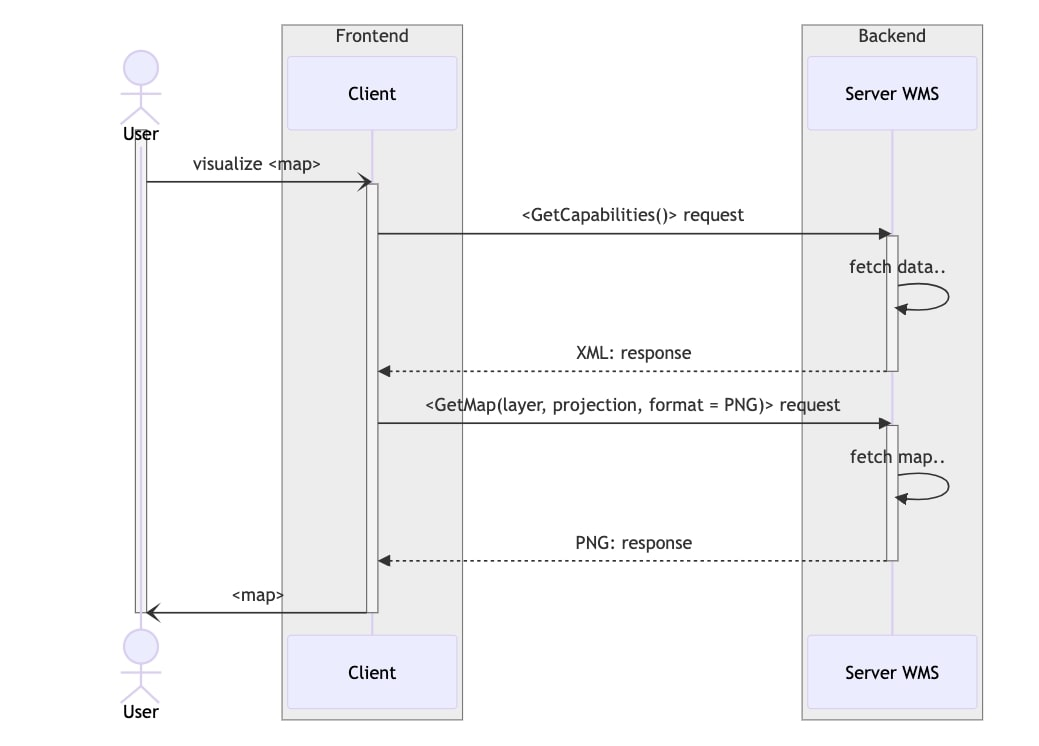
\includegraphics[width=1\textwidth]{images/Capitolo2/ProtocolWMS.jpg}
      \caption{Diagramma di Sequenza del protocollo WMS}
      \label{fig:wms protocol}
\end{figure}

\subsubsection{Formato della richiesta}

Lo standard specifica diversi tipi di richieste che possono essere effettuate ai server WMS:
\begin{itemize}
      \item \textit{GetCapabilities}: questa richiesta restituisce un documento XML che rappresenta le informazioni sul servizio WMS stesso. Nello specifico, fornisce l'elenco dei layer disponibili, le proiezioni supportate, i bounding box (rispettivi per ogni proiezione), la versione del protocollo WMS supportata, gli stili delle mappe disponibili e un abstract che fornisce una descrizione della mappa.     
      \item \textit{GetMap}: utilizzata per ottenere un'immagine di mappa dal servizio. I parametri inclusi nella richiesta comprendono: il nome del layer, la versione del protocollo utilizzato, lo stile, la proiezione, i bounding box, il formato e la larghezza e altezza dell'immagine in pixel. La risposta alla richiesta è un'immagine della mappa, pronta per essere visualizzata su un browser web o in un'applicazione client.
\end{itemize}
I tipi di richiesta che i fornitori di WMS possono opzionalmente supportare includono:
\begin{itemize}
      \item \textit{GetFeatureInfo}: consente di ottenere informazioni dettagliate su specifiche caratteristiche presenti sulla mappa. Restituisce informazioni associate a quella posizione, come punti di interesse o dati geografici particolari.
      \item \textit{DescribeLayer}: restituisce i tipi di feature disponibili per i layer specificati, che possono essere ulteriormente descritti utilizzando richieste Web Feature Service (WFS). Questa richiesta è utile per comprendere meglio la struttura e le caratteristiche dei dati geospaziali presenti nel servizio WMS.
      \item \textit{GetLegendGraphic}: utilizzata per ottenere un'immagine della legenda della mappa, questa richiesta fornisce una guida visiva agli elementi presenti sulla mappa, come i simboli e le etichette dei layer.
\end{itemize}
Qui sotto è riportato uno snippet che contiene alcuni esempi possibili di richieste WMS, eseguite utilizzando il comando cURL per simulare il comportamento di una richiesta HTTP.
\lstinputlisting[language=bash]{listings/Capitolo2/wms-requests-example.sh}
Qui di seguito invece viene mostrato al lettore un esempio di richiesta funzionante, fatta durante il percorso di tirocinio, ai server WMS del Geoportale Nazionale, gestito dal Ministero dell'Ambiente e della Sicurezza Energetica.
Ciò serve per ottenere dati geospaziali relativi alla mappa che illustra l'area allagabile conforme al Piano di Gestione del Rischio di Alluvioni (PGRA) del 2021.
\lstinputlisting[language=bash]{listings/Capitolo2/wms-requests.sh}
Come si può vedere dal messaggio di risposta \cite{GetCapabilitiesWMS} in formato XML inviato dai loro Server,
il servizio offre funzionalità standard come la richiesta di mappe (GetMap) e informazioni (GetFeatureInfo), oltre a supportare la descrizione dei layer (DescribeLayer) e la visualizzazione della legenda (GetLegendGraphic).
\\Per ulteriori informazioni dettagliate sullo standard WMS, è possibile fare riferimento alla documentazione ufficiale disponibile sul sito web di Open Geospatial Consortium \cite{DocumentazioneWMS}

\subsection{Protocollo WMTS}

A differenza del WMS, il quale invia un'unica immagine per ogni mappa ai client, il WMTS la "segmenta" in piccole porzioni rettangolari, denominate \textit{tiles}. Queste ultime vengono prima pre-renderizzate e poi memorizzate sul server. Successivamente, sotto richiesta dei client, vengono recuperate e restituite come messaggio di risposta. 
\\Nello specifico, quando un client desidera visualizzare una mappa, invia al server WMTS tante richieste HTTP differenti per ogni tiles che vuole ottenere. Ciascuna richiesta contiene al suo interno: la porzione di mappa, la proiezione e il formato di immagine desiderato. Il server, per ogni richiesta HTTP ricevuta, risponde di conseguenza, inviando al client le tiles. A questo punto il client, una volta ottenute le tiles, le combina insieme per formare la porzione di immagine di mappa richiesta.
\\Una delle principali caratteristiche del WMTS è che l'utilizzo delle tiles riduce la quantità di elaborazione necessaria al server per mostrare correttamente la mappa. Il server WMTS deve infatti fornire solo le tiles necessarie per l'area richiesta e può riutilizzare parti di mappa già calcolate in precedenza, anziché generare e inviare tutte le volte un'unica immagine completa.
\\Inoltre, l'utilizzo di tiles facilita l'implementazione di una politica di caching, in quanto essendo piccole porzioni di immagini, queste possono essere memorizzate facilmente. Sul lato back-end, infatti, il servizio WMTS può memorizzare nella cache le tiles più utilizzate e restituirle più rapidamente al client. Lato front-end, invece, il browser è in grado di intercettare le risposte inviate dal server e di memorizzare nella sua cache interna l'immagine della tile. In questo modo, quando il client richiede la stessa tile, quest'ultima viene visualizzata senza dover contattare nuovamente il server. Diversamente, nel protocollo WMS, risulta essere più complesso implementare il meccanismo di caching a causa dei parametri che vengono utilizzati nelle richieste di GetMap. I query params di tale richiesta, infatti, risultano essere molto più variabili, specialmente con il parametro Bounding Box che cambia ogni qualvolta che si visualizza una porzione geografica differente.

\begin{figure}[htbp]
      \centering
      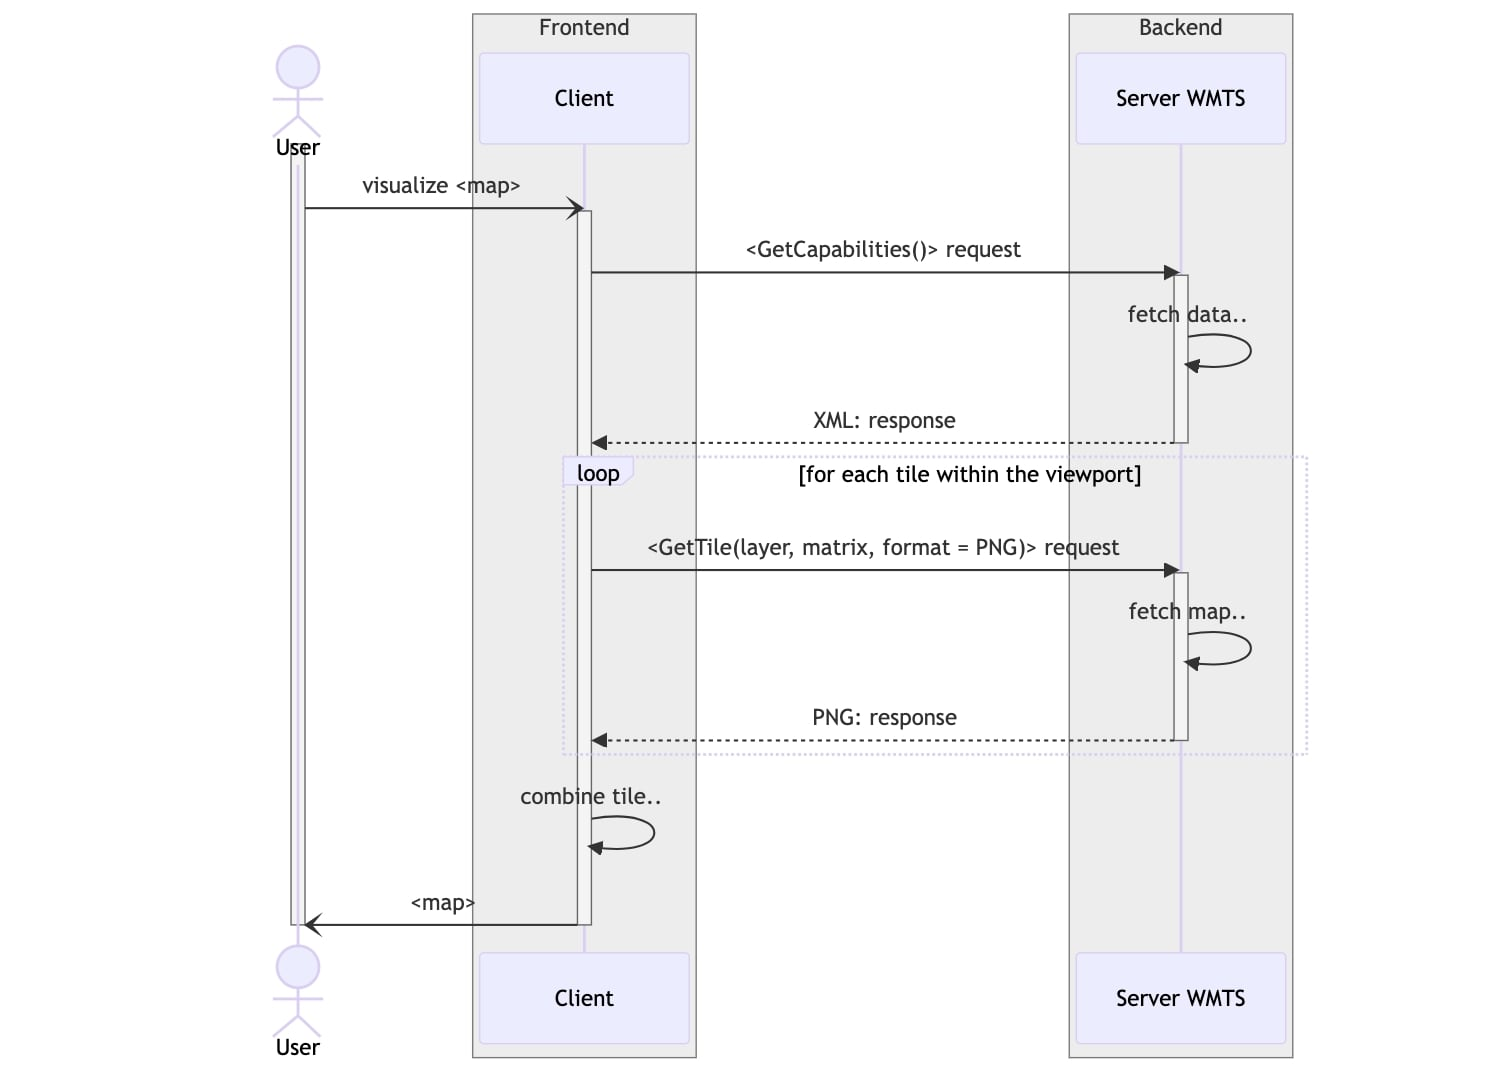
\includegraphics[width=1\textwidth]{images/Capitolo2/ProtocolWMTS.jpg}
      \caption{Diagramma di Sequenza del protocollo WMTS}
      \label{fig:wmts protocol}
\end{figure}

\subsubsection{Formato della richiesta}

\begin{itemize}
      \item \textit{GetCapabilities}: Restituisce un documento XML che descrive il \textit{Manifest} del servizio WMTS, inclusi i layers disponibili, i formati supportati, le coordinate di riferimento e altro ancora.
      \item \textit{GetTile}: Restituisce una Tile specifica in base alle coordinate geografiche e allo zoom specificato nella richiesta.
      \item \textit{GetFeatureInfo}: Questa richiesta non è molto comune nei servizi WMTS, in quanto generalmente viene direttamente utilizzata la richiesta GetFeatureInfo fornita dal servizio WMS. Se abilitata, questa richiesta restituisce informazioni aggiuntive associate a una tile, come attributi dei dati geospaziali presenti in quel punto della mappa.
\end{itemize}
Qui di seguito è riportato uno \textit{snippet} contenente alcuni esempi possibili di richieste WMTS, eseguite utilizzando il comando cURL per simulare il comportamento di una richiesta HTTP.

\lstinputlisting[language=bash]{listings/Capitolo2/wmts-requests-example.sh}
Per ulteriori informazioni dettagliate sullo standard WMTS, è possibile fare riferimento alla documentazione ufficiale disponibile sul sito web di Open Geospatial Consortium \cite{DocumentazioneWMTS}

\subsection{Protocollo WFS}

Il Web Feature Service (WFS) è un servizio web utilizzato per accedere e manipolare dati geospaziali attraverso internet. La differenza principale tra un servizio WMS e WFS risiede nel tipo di dati che vengono trasmessi e nel modo in cui vengono rappresentati dal client.
\\Come già spiegato, il servizio WMS si occupa principalmente di offrire una rappresentazione visiva delle informazioni geografiche, distribuendo le mappe principalmente sotto forma di immagini raster o vettoriali. Quest'ultime sono già pronte per essere visualizzate e non richiedono ulteriori elaborazioni: il client dovrà soltanto rappresentarle nella corretta proiezione.
\\Un WFS trasmette dati geospaziali grezzi, come numeri, coordinate e altre proprietà, che devono essere interpretati e visualizzati dal client. Ciò significa che sarà compito del client elaborare questi dati e rappresentarli come mappa con uno specifico stile grafico, disegnando ad esempio punti, linee o poligoni secondo le specifiche della visualizzazione desiderata. Tali dati, che prendono il nome di "Feature", sono dati geospaziali vettoriali che vanno a rappresentare oggetti geografici reali come per esempio strade, fiumi o frane. Ogni feature possiede al proprio interno un insieme di attributi che definiscono il suo tipo di geometria e la sua posizione sulla mappa. Inoltre, una Feature può includere ulteriori proprietà che forniscono più informazioni sulla feature stessa, come ad esempio: nome, altezza, larghezza, regione, etc...
\\Per comprendere meglio la differenza, qui di seguito è riportato un esempio Feature, nel formato geospaziale GeoJSON che è stato utilizzato durante il tirocinio.
\lstinputlisting[language=JSON]{listings/Capitolo2/exampleGeoJson.json}
Similmente al WMS, che attraverso la richiesta GetMap può richiede una mappa specifica al server, il servizio WFS offre la richiesta GetFeature per richiedere una feature precisa che il server WFS provvederà a fornirgli.
\\I client possono anche eseguire operazioni di analisi spaziale, come il calcolo dell'area di un poligono o la ricerca delle feature più vicine a una determinata posizione.
Ad esempio, è possibile interrogare il servizio per ottenere informazioni su tutti gli edifici situati in una determinata area, oppure trovare tutti i fiumi di una certa lunghezza.
\\Queste informazioni vengono trasmesse utilizzando il formato GML (Geography Markup Language), ovvero un formato basato su XML che consente di descrivere in modo dettagliato la geometria e le proprietà di ciascuna feature. Ciò non toglie che i servizi WFS possano supportare anche altri tipi di formati, come il GeoJSON. In questo caso sarà dovere del server, definire all'interno delle informazioni presenti nella richiesta di GetCapabilities, tutti i formati geospaziali supportati. A quel punto il client, potrà richiedere il tipo di formato desiderato specificandolo nei queryParams (per esempio \textit{outputFormat=application/json}).

\begin{figure}[htbp]
      \centering
      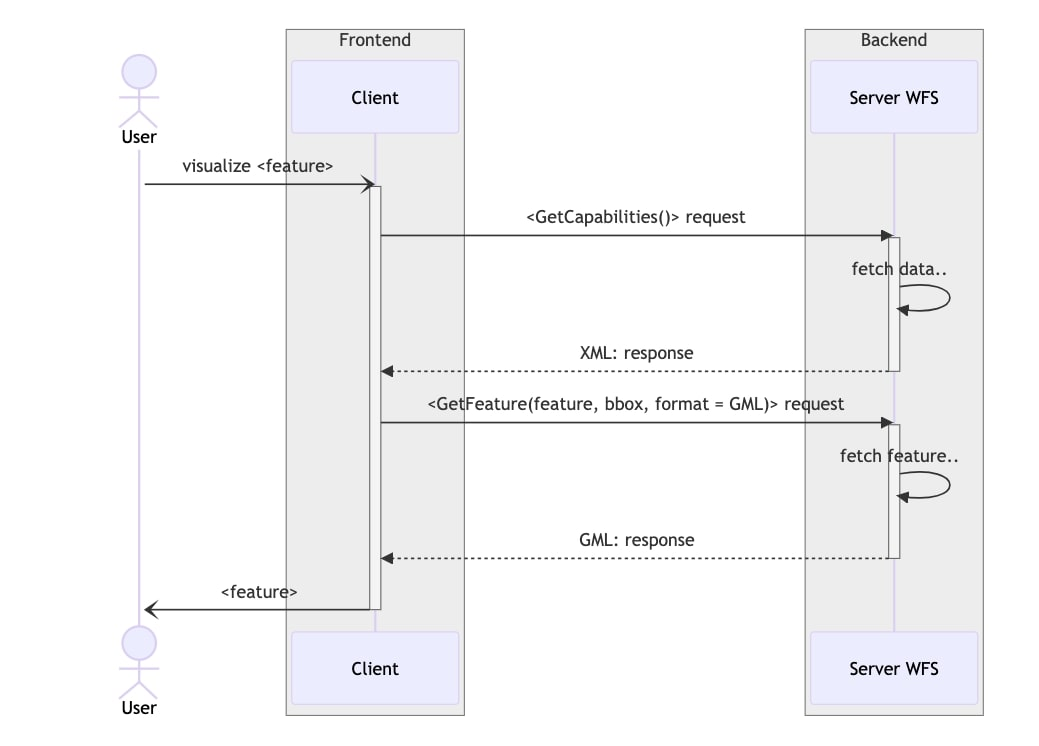
\includegraphics[width=1\textwidth]{images/Capitolo2/ProtocolWFS.jpg}
      \caption{Diagramma di Sequenza del protocollo WFS}
      \label{fig:wfs protocol}
\end{figure}

\subsubsection{Formato della richiesta}

Le richieste che è possibile fare a un servizio WFS (Web Feature Service) sono le seguenti:

\begin{itemize}
      \item \textit{GetCapabilities}: Come per i WMS, la richiesta GetCapabilities restituisce un documento XML che fornisce informazioni dettagliate sul servizio WFS stesso. Queste informazioni includono i tipi di feature disponibili, i formati di trasmissione dei dati supportati (GML, GeoJSON, ecc..), i tipi di richieste supportate, le proiezioni geografiche disponibili e altre capacità del servizio.
      \item \textit{GetFeature}: è la richiesta principale nel protocollo WFS in quanto consente agli utenti di recuperare la feature interessata. I parametri inclusi nella richiesta comprendono il nome della feature, il tipo di formato desiderato, la sua proiezione, ecc..
      \item \textit{DescribeFeatureType}: è usata per richiede informazioni su un singolo tipo di feature prima di chiedere effettivamente la feature stessa. In particolare, l'operazione richiede un elenco di feature e attributi per il tipo di feature dato, oppure un elenco dei tipi di feature disponibili.
\end{itemize}
I tipi di richiesta che i servizi WFS possono opzionalmente supportare sono:
\begin{itemize}
      \item \textit{Transaction}: consente agli utenti di modificare i dati geografici nel servizio WFS, attraverso le operazioni come inserimento, modifica o eliminazione di una feature. Ciò è utile per gli utenti che hanno bisogno di mantenere aggiornati i dati geografici all'interno del servizio, consentendo loro di interagire direttamente e apportare modifiche in tempo reale.
      \item \textit{GetPropertyValue}: questa richiesta consente agli utenti di ottenere i valori degli attributi di una o più feature, senza recuperarne tutti i dettagli geometrici associati.
      \item \textit{LockFeature}: consente agli utenti di acquisire una lock di accesso in mutua esclusione alla feature, impedendo ad altri utenti di modificarla contemporaneamente.
      \item \textit{GetFeatureWithLock}: questa richiesta combina le funzionalità di GetFeature e LockFeature. In questo modo è possibile acquisire una lock di accesso in mutua esclusione alla feature desiderate prima di richiedere la feature stessa.
\end{itemize}
Qui di seguito è riportato uno \textit{snippet} contenente alcuni esempi possibili di richieste WFS, eseguite utilizzando il comando cURL per simulare il comportamento di una richiesta HTTP.

% \texttt{WFS example requests}.
\lstset{basicstyle=\footnotesize\ttfamily}
\lstinputlisting[language=bash]{listings/Capitolo2/wfs-requests-example.sh}
Ecco un altro esempio di richiesta funzionante, effettuata sempre durante il percorso di tirocinio, ai server WFS del Geoportale Nazionale.
Come si può notare, questa richiesta è simile a quella effettuata precedentemente per il servizio WMS, ma questa volta viene rivolta al servizio WFS. Entrambi i servizi offrono informazioni sulla stessa mappa, ma con approcci diversi: mentre il WMS fornisce immagini della mappa, il WFS trasmette le feature geospaziali che compongono la mappa.

\lstset{basicstyle=\footnotesize\ttfamily}
\lstinputlisting[language=bash]{listings/Capitolo2/wfs-requests.sh}
Anche in questo caso, come si può vedere dal loro messaggio di risposta \cite{GetCapabilitiesWFS} in formato XML inviato dai loro Server,
il servizio offre funzionalità standard come la richiesta di feature (GetFeature) e la descrizione dei tipi di feature (DescribeFeatureType), oltre a supportare la modifica dei dati geografici tramite transazioni (Transaction).
\\Per ulteriori informazioni dettagliate sullo standard WFS, è possibile fare riferimento alla documentazione ufficiale disponibile sul sito web di Open Geospatial Consortium \cite{DocumentazioneWFS}

\section{Tiled Map Service (TMS)}

Il protocollo Tiled Map Service (TMS), è un altro standard utilizzato per servire mappe geospaziali. A differenza di quelli sopra citati, questa specifica non è definita dall'Open Geospatial Consortium, ma è stata introdotta dall'Open Source Geospatial Foundation (OSGeo). Per questo motivo, nonostante entrambi i protocolli si occupano di fornire dati di mappe, presentano delle differenze.
\\Questo standard può essere considerato come una versione più "leggera" del servizio WMTS, in quanto continua a servire mappe sotto forma di tiles, ma offre contemporaneamente meno funzionalità.
Infatti, questo standard non richiede che il client debba prima ottenere informazioni sul servizio attraverso una richiesta simile a GetCapabilities, ma può può dedurre queste informazioni dalla struttura dell'URL stesso. Il client, infatti, può accedere direttamente alle tiles della mappa tramite percorso URL, in cui ogni tiles è rappresentata da un percorso differente.
Si può dunque affermare che la struttura degli URL di un servizio TMS segue una convenzione simile a quella delle cartelle: ogni livello di zoom della mappa e ogni tile è rappresentata da un URL univoco e questi possono essere organizzati in modo gerarchico, nello stesso modo delle cartelle in un File System.
\\Questo comporta da un lato un protocollo più semplice, ma dall'altro meno funzionalità: ad esempio, il servizio non può fornire informazioni su tutti i tipi di richieste a cui può essere interrogato. Nel caso di un servizio WMS, il client attraverso GetCapabilities può capire o meno se il server supporta ulteriori richieste come GetFeatureInfo o GetLegendGraphic.
Inoltre, il protocollo TMS prevede solo la trasmissioni di immagini tile, non restituisce altri tipi di informazioni (come nel caso della GetLegendGraphic che restituisce l'immagine della legenda associata allo stile della mappa).
\\Ciò può sembrare una cosa negativa, ma è importante tenere conto anche del peso delle richieste. Una richiesta di GetCapabilities ad un servizio di mappe può restituire un messaggio di risposta molto grande e pesante, sopratutto se contiene molti layer (mappe) al suo interno. Durante il tirocinio è capitato per esempio di ricevere risposte di un peso oltre i 30MB. Anche se può sembrare insignificante, gestire un peso simile all'interno di servizi web risulta molto tedioso, specialmente dal punto di vista della memorizzazione nella cache del browser.
\\Inoltre, avere una struttura gerarchica simile a quella di un File System, può portare a tanti benefici. Uno di essi, ad esempio, è la facilità nel distribuire tutte le tiles tramite una CDN (Content Delivery Network) in modo elementare. La stessa cosa può essere fatta anche nel caso dei servizi WMTS tramite query params, ma risulta molto più complesso e difficile da gestire.
Utilizzando il protocollo TMS, infatti, è possibile archiviare le tiles in uno storage generico e servirle senza la necessità di elaborare nuovamente le richieste in ingresso. Ad esempio, su AWS, questa operazione può essere eseguita utilizzando lo storage S3 e la CDN CloudFront, entrambi privi di meccanismi specifici per la gestione dei dati o dei protocolli GIS. Questo approccio consente un miglior bilanciamento del carico sul server, permette di offrire la stessa mappa su più istanze contemporaneamente e garantisce la continuità del servizio.
\\Infine, le richieste di un servizio TMS sono più facili da memorizzare nella cache del browser rispetto al WMTS perché i suoi URL sono semplici e diretti. Al contrario, il WMTS spesso utilizza parametri più complessi nelle sue richieste, attraverso l'utilizzo dei query parameters, rendendo la memorizzazione nella cache del browser meno diretta e più soggetta a variazioni.
\\La struttura di una richiesta TMS per accedere ad una specifica tile è la seguente
\lstinputlisting[language=bash]{listings/Capitolo2/tms-requests-example.sh}
Questa richiesta restituisce direttamente una tile della mappa, generalmente grande 256x256, nel formato e proiezione richiesti. Le coordinate x e y rappresentano la posizione della tile all'interno della griglia, mentre la z il suo livello di zoom. Per ogni livello di zoom sono presenti dei confini, chiamati "Bounding Box" o "extent" che indicano l'estensione geografica delle tiles disponibili per quel livello di zoom. Se vengono richieste delle tile al di fuori di questi confini, il server TMS restituisce ovviamente un messaggio di errore.
\begin{figure}[htbp]
      \centering
      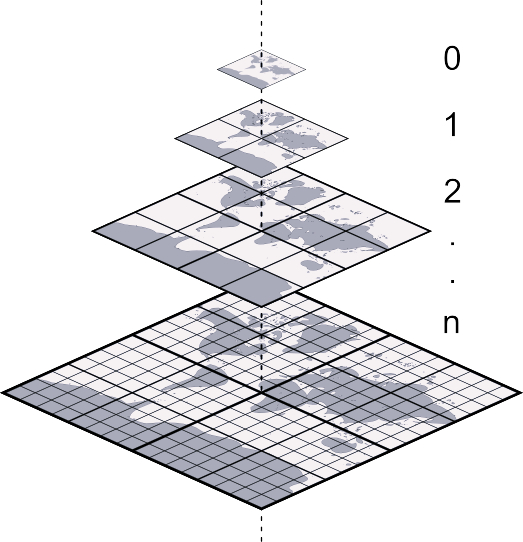
\includegraphics[width=0.5\textwidth]{images/Capitolo2/tilesPyramid.jpg}
      \caption{Tiles con livello di zoom}
      \label{fig:tmsTiles}
\end{figure}

\subsubsection{Formato della richiesta}

Come indicato nella specificata del servizio TMS \cite{DocumentazioneTMS}, esistono anche altre richieste che un client può effettuare per ottenere ulteriori informazioni oltre a quella relativa alle tiles. Le principali sono:
\begin{itemize}
      \item \textit{TileMapServiceResource}: questa richiesta è quella più simile a GetCapabilities, permette di vedere tutte le mappe disponibili che il servizio TMS ha a disposizione, specificando il nome della mappa, il formato dell'immagine e la sua proiezione. Può anche essere fornita più volte la stessa mappa, con formati e proiezioni differenti. Un esempio di risposta a tale richiesta è la seguente:
            \lstset{basicstyle=\footnotesize\ttfamily}
            \lstinputlisting[language=xml]{listings/Capitolo2/TileMapServiceResource.xml}
      \item \textit{TileMapResource}: questa richiesta fornisce informazioni più dettagliate su una mappa, specificandone i confini, la dimensione delle tile, la proiezione e tutti i livelli di zoom disponibili che il client può richiedere (coordinata z) con i suoi rispettivi confini (extent). Un esempio di risposta a tale richiesta è la seguente:
            \lstset{basicstyle=\footnotesize\ttfamily}
            \lstinputlisting[language=xml]{listings/Capitolo2/TileMapResource.xml}
      \item \textit{TileResource}: la richiesta effettiva per richiedere la tile che corrispondete esattamente a quella spiegata in precedenza.
\end{itemize}
Il ciclo di vita di un client che richiede una mappa da un server TMS può essere descritto nel seguente modo:
inizialmente, il client contatta tramite richiesta TileMapServiceResource un server TMS per ottenere le informazioni di tutte le mappe disponibili.
Dopo aver selezionato la mappa desiderata, il client utilizza la richiesta TileMapResource per ottenere tutti i possibili livelli di zoom, con i relativi confini.
A questo punto il client richiede direttamente le tiles della mappa desiderata attraverso le coordinate x, y e z, senza sforare dai confini. Il server risponde risponde con l'immagine della tile.

\section{Formati di file Geospaziali}
I formati di file geospaziali sono tipi di file che vengono utilizzati per memorizzare e scambiare dati geografici. Questi dati possono includere informazioni come mappe, immagini satellitari, dati di altitudine, di utilizzo del suolo e molti altri. Alcuni dei formati di file geospaziali più comuni includono:
\begin{itemize}
      \item \textit {Shapefile} (.shp): è uno dei formati più diffusi per memorizzare dati geografici vettoriali, come punti, linee e poligoni.
      \item \textit {GeoTIFF} (.tif): è una versione del formato di file di immagini TIFF (Tagged Image File Format) e viene usato per rappresentare principalmente immagini raster geografiche.
      \item \textit {GeoJSON} (.json): è un formato di file basato su JSON (JavaScript Object Notation) e similmente allo Shapefile, è utilizzato per memorizzare dati geografici vettoriali. Questo formato è spesso utilizzato per lo scambio di dati geografici tramite protocollo HTTP.
      \item \textit {KML/KMZ} (.kml, .kmz): KML (Keyhole Markup Language) è un formato di file XML utilizzato per memorizzare dati geografici ed ha una sua versione compressa nota con il nome di KMZ.
      \item \textit {GeoPackage} (.gpkg): è un formato che memorizza i dati geospaziali utilizzando il linguaggio SQL per gestire e interrogare i dati contenuti al suo interno, sia vettoriali che raster.
\end{itemize}
La diversità di formati esistenti non costituisce un problema per i client che necessitano di utilizzare dati geospaziali. 
Normalmente, si tende a conservare sui server i dati di mappe nei formati sopra citati. 
\\Un server di mappe, a sua volta, può quindi supportare contemporaneamente più servizi (WMS, WMTS, WFS, TMS, etc...).  Questo perché ciascun server di mappe è in grado di convertire gli stessi dati iniziali in formati diversi, solitamente quelli richiesti dai client attraverso il protocollo da loro scelto.
\\Ad esempio, un server WMS permette di richiedere una mappa in formato PNG o JPG. Quando viene effettuata una richiesta tramite questo servizio, il server accede ai suoi dati, ad esempio degli Shapefile, li converte nel formato specificato (PNG o JPG) e li restituisce al client che li aveva richiesti.
È da notare come non ci si debba necessariamente attenere ad uno dei protocolli standard esistenti, ma si possa anche specificarne uno personalizzato che permetta di restituire i dati iniziali in un formato scelto a proprio piacimento. Ad esempio, si potrebbe realizzare un protocollo che restituisce i dati direttamente nel loro formato originario.

\section{Software utilizzati}

L'integrazione dei protocolli OGC è stata resa possibile mediante l'utilizzo di due tecnologie distinte, le quali hanno svolto un ruolo specifico all'interno del progetto di tirocinio.
\\Per la parte di sviluppo front-end, si è fatto uso di OpenLayers, una libreria JavaScript che permette di realizzare interfacce grafiche per la visualizzazione di mappe geospaziali. Quest'ultima offre, in maniera basilare, una mappa interattiva con delle funzionalità già implementate, come ad esempio lo zoom e l'interazione con elementi a schermo, e delle API ad alto livello, che permettono di utilizzare i protocolli sopra menzionati. Un'analisi dettagliata sull'implementazione di questa libreria e le motivazioni che hanno portato alla sua adozione all'interno del progetto, sono approfondite nel capitolo \ref{cap:chapter4}.
\\Fra tutti gli elementi componenti il back-end invece, al fine di risolvere alcuni problemi implementativi riscontrati durante il tirocinio, è stato introdotto un nuovo software, denominato GeoServer. Quest'ultimo permette di memorizzare al suo interno, anche se in maniera laboriosa e complessa, dati di mappe geospaziali e permette di servirli utilizzando i protocolli appena descritti. Le scelte che hanno portato al suo impiego e il suo funzionamento sono approfondite nel capitolo \ref{cap:chapter5}. La modalità con cui viene risolta la complessità legata all'inserimento delle mappe, invece, viene spiegata nel capitolo \ref{cap:chapter6}.

\chapter{Tecnologie aziendali utilizzate}
\label{cap:chapter3}

Questo capitolo si propone di fornire una panoramica generale sulle tecnologie e i software utilizzati nell'architettura del progetto, nonché quelli adoperati dall'azienda stessa. L'obiettivo è quello di comprendere più approfonditamente le scelte progettuali adottate durante il percorso lavorativo del candidato.

\subsection{Microservizi e Docker}

La piattaforma, che prende l'acronimo di \textit{BMS} (\textit{Bridge Management System}) è stata sviluppata come un'applicazione Web moderna, seguendo un'architettura a microservizi che favorisce la modularità e la scalabilità del sistema. Questa scelta architetturale è stata preferita rispetto alle tradizionali applicazioni monolitiche, in quanto ha permesso di separare i vari servizi, semplificandone la gestione e consentendo una maggiore flessibilità nell'implementazione di nuove funzionalità.
\\Questo approccio è molto comune per le applicazioni di grandi dimensioni, poiché ogni microservizio può essere sviluppato e mantenuto in modo indipendente dagli altri, utilizzando, se necessario, anche linguaggi di programmazione differenti. Tale sistema permette agli sviluppatori di concentrarsi su ogni funzionalità singolarmente, rimanendo isolati da tutto il resto dell'applicazione. Inoltre, grazie alla possibilità di utilizzare linguaggi differenti, è possibile scegliere la soluzione più adatta in base alla funzionalità che deve essere implementata. Quest'architettura favorisce la scalabilità orizzontale, ovvero la possibilità di aggiungere o rimuovere istanze di singoli microservizi in base alle esigenze di carico, senza dover scalare l'intera applicazione. Dunque, rende più efficiente l'utilizzo delle risorse e consente di gestire picchi di traffico in modo più efficace.
\\Per gestire questo tipo di architettura, si è scelto di utilizzare Docker, ovvero una piattaforma che consente di creare e gestire container, cioè ambienti isolati che contengono tutte le risorse necessarie per eseguire un'applicazione.
Ogni servizio viene dunque "containerizzato", ovvero viene isolato in un ambiente autonomo con tutte le risorse e le dipendenze necessarie per il suo funzionamento. La containerizzazione attraverso Docker rende notevolmente più semplice lo sviluppo dell'applicazione, in quanto gli sviluppatori, lavorando sullo stesso container, possiedono tutti lo stesso ambiente di sviluppo: la stessa versione delle dipendenze, librerie e del linguaggio di programmazione. Inoltre, una volta che l'applicazione è pronta per il deployment (cioè pronta per essere messa in produzione), viene eseguita su server in un ambiente ancora containerizzato. Così facendo, si ha la garanzia che l'applicazione continui a funzionare come quando è stata sviluppata, e, se necessario, è possibile scalarla orizzontalmente attraverso l'uso di servizi Cloud come Amazon AWS.

\subsection{WebServer e Reverse Proxy}

È stato impiegato un WebServer che, tra le altre cose, ha svolto il ruolo di un Reverse Proxy, permettendo di semplificare la gestione del traffico HTTP diretto verso i container Docker. Un WebServer è un software che riceve tutte le richieste HTTP inviate da client (per esempio browser) e che alla fine fornirà loro delle risposte, solitamente sotto forma di dati o pagine web.
\\Comportandosi da reverse proxy, il WebServer reinstrada le richieste ricevute verso il microservizio appropriato, mascherando ai client la pluralità di servizi esistenti. Una volta ricevuta la risposta dal microservizio, la trasmette al client che ne aveva fatto richiesta. Nel dettaglio è stato utilizzato Caddy come WebServer, poiché offre delle semplici modalità di configurazione, tramite la stesura del file "Caddyfile", fornito dal software stesso. 
\\Il suo uso principale è stato quello di permettere ai client di contattare i servizi containerizzati tramite un dominio, anziché un indirizzo ip con una porta associata: ad esempio, invece di contattare il container che ha al suo interno il servizio di rest API all'indirizzo \textit{127.0.0.1:8080}, è possibile contattarlo tramite il dominio \textit{bms.local.gkops.net/api/}. Grazie a questa modalità, è possibile simulare un ambiente di produzione, nel quale tutti i servizi vengono contattati su un dominio apposito tramite protocollo HTTPS. Quest'ultimo dettaglio è possibile grazie a Caddy che permette di installare certificati TLS sui domini da lui creati. È stato utilizzato Let's Encrypt come Certification Authority.
\\Inoltre, se necessario, tramite Caddy è possibile eseguire load balancing tra i microservizi, il quale consente di distribuire il carico tra più istanze del servizio per garantire una migliore scalabilità e affidabilità del sistema.
\\Infine, l'utilizzo di Caddy è essenziale per effettuare meccanismi di caching tra le richieste HTTP inviate dai client ai microservizi: nel caso in cui venga posta la medesima richiesta, il WebServer non richiederà nuovamente al il microservizio la risposta, bensì risponderà direttamente al client.

\subsection{Front-end e Back-end}

Per quanto concerne le tecnologie impiegate nello sviluppo dell'interfaccia grafica della piattaforma, è stato selezionato \textit{Angular}, un framework JavaScript moderno e robusto, caratterizzato da una struttura modulare che offre una vasta gamma di librerie. Queste caratteristiche lo rendono particolarmente adatto per la creazione di interfacce utente dinamiche e complesse, richieste proprio da progetti di questo tipo.
\\Questi framework presentano un'architettura basata su componenti, cioè permettono di costruire l'interfaccia grafica attraverso l'uso di componenti che possono essere riutilizzati. Questo consente di avere una programmazione modulare, in cui ogni componente HTML viene visto come un modulo a sé stante, che può essere importato e riutilizzato su pagine web differenti. Questo rende il codice più organizzato, facile da comprendere e da mantenere, specialmente all'aumentare delle dimensioni e della complessità dell'applicazione.
\\Lato back-end, invece, è stato adottato l'utilizzo di un framework ad alto livello come .NET, il quale offre un insieme di funzionalità e strumenti per lo sviluppo di applicazioni complesse e scalabili.
\\L'adozione di Angular e .NET come principali framework di sviluppo hanno consentito agli sviluppatori di seguire un pattern unificato attraverso una varietà di progetti. Questa scelta ha ridotto la confusione e ha garantito una maggiore coerenza nelle implementazioni, assicurando che tutti i software sviluppati seguissero gli stessi standard e convenzioni. Si tratta di un aspetto cruciale in contesti aziendali con molti progetti in corso, in quanto si facilita la gestione e la manutenzione dell'intero insieme di software.
\\Infine, nella comunicazione tra front-end e back-end della piattaforma, è stato adottato il paradigma delle \textit{Rest API}, che rappresenta uno standard per lo scambio di dati tra client e server su protocollo HTTP. Più specificamente, le API sono esposte tramite Swagger UI, consentendo al front-end di interagire con esse in modo intuitivo e documentato. Il protocollo utilizzato per definire le specifiche delle API rispecchia lo standard di OpenAPI 3 (OAS3), garantendo una chiara e precisa descrizione delle operazioni e dei dati scambiati tra front-end e back-end.

%\subsection{Reactive Programming e Angular}

%Si è poi proseguito con lo studio della libreria RxJS, fondamentale per l'uso di Angular, in quanto è parte integrante dello stesso.
%Tale libreria viene utilizzata internamente da Angular per gestire numerose operazioni asincrone attraverso l'uso di Stream, adottando il paradigma di "Reactive Programming" invece che "Event Driven".
%\\Nel paradigma a eventi, viene scritto del codice per gestire un evento quando questo si verifica. In genere si definisce una funzione, nota come callback, che viene registrata su un certo evento. Quando tale evento si verifica, come ad esempio un click del mouse su un pulsante, la funzione registrata viene invocata per gestire l'evento di click.
%Nell'approccio reattivo, invece, viene scritto del codice per gestire uno Stream di dati che rappresenta una sequenza continua di eventi. Ad esempio, invece di gestire il singolo click del mouse, viene creato uno Stream che rappresenta i click che avvengono del tempo. Tale Stream può essere manipolato, filtrato o trasformato utilizzando degli operatori.
%\\Angular utilizza RxJS per adottare quest'ultimo tipo di paradigma, facendo uso di tre elementi interdipendenti: l'Observable, gli Operator e gli Observer.
%\\L'Observable è colui che fornisce i dati sullo Stream ed è colui che è oggetto dell'osservazione. Durante il fornimento dei dati, che avviene in maniera continua nel tempo, gli Operator si occupano di manipolarli. Gli Operator sono delle operazioni che permettono la manipolazione dei dati sullo Stream in maniera asincrona. Le operazioni più note sono la mappatura, il filtraggio, la combinazione e la trasformazione. L'Observer si trova alla fine della catena e si occupa di utilizzare il risultato dei dati elaborati.
%\\Angular utilizza internamente gli Observable a basso livello per gestire i suoi componenti, mentre ne espone un'interfaccia semplificata ad alto livello per l'utilizzo da parte degli sviluppatori. Ad esempio, il routing delle pagine web e il modulo del form di input fanno uso degli Observable per monitorare e rispondere agli eventi di input dell'utente.
\chapter{Sviluppo Front-end con OpenLayers}
\label{cap:chapter4}

In questo capitolo verrà esaminato in dettaglio il funzionamento della libreria di OpenLayers e le ragioni che hanno portato alla sua scelta come strumento principale per l'implementazione delle mappe nell'ambito del progetto. Successivamente, saranno poi esposte le prime implementazioni, ancora prive di un back-end, realizzate dal candidato con questa libreria, ponendo l'attenzione su tutte le problematiche da lui riscontrate fino al raggiungimento di una soluzione.

\section{Introduzione a OpenLayers}

OpenLayers è una libreria open source JavaScript che fornisce strumenti per la visualizzazione di mappe interattive su pagine web. Fornisce grande capacità di astrazione per gli sviluppatori, andando ad incapsulare tutte le funzionalità dei servizi menzionati fino ad ora. 

\subsection{Caratteristiche principali}
Una delle caratteristiche principali di OpenLayers è la sua capacità di offrire un interfaccia grafica di mappe omogenea su diversi tipi di dispositivi e browser. Essa permette, in modo intuitivo e conciso, di accedere a una serie di funzionalità basilari, quali zoom, capacità di trascinare la mappa e interazione con elementi a schermo (come marker o punti).
\\Offre inoltre API ad alto livello che consentono di integrare facilmente diversi tipi di servizi geospaziali nei progetti, come WMS, WMTS, WFS, TMS etc...
Sono supportati anche formati strettamente geospaziali, tra cui GeoJSON, KML, etc... L'accesso a questi dati è possibile sia contattando un server esterno, senza aver bisogno di utilizzare esplicitamente i servizi sopra citati, sia salvando i relativi file direttamente in locale per poi accedervi.
\\Infine, OpenLayers supporta di default alcuni provider di mappe, tra cui: OpenStreetMap, Bing Maps, Google Maps, etc... Ciò non preclude la possibilità di utilizzare altri servizi di mappe esterni.

\subsection{Architettura di OpenLayers}

Il lavoro di tirocinio è iniziato con lo studio e l'utilizzo di tale libreria, partendo dalla creazione di una piccola applicazione esterna al progetto aziendale. Questa scelta è stata fatta per acquisire una comprensione approfondita del suo funzionamento, in modo poi da poterla poi confrontare con la versione già iniziata dall'azienda. In questo procedimento, il candidato ha deciso di privare tale applicazione del framework Angular e di librerie di terze parti, così da semplificare il suo utilizzo.
\\Lo studio da parte del candidato è quindi cominciato con la consultazione della documentazione ufficiale \cite{DocumentazioneOpenLayersBase}, la quale riporta i quattro componenti principali su cui si basa OpenLayers:
\begin{itemize}
    \item ol/Map: è il core della libreria, rappresenta la mappa stessa e fornisce funzionalità di base come la gestione dei layer, degli eventi e delle view.
    \item ol/View: si occupa di gestire la View (la vista) della mappa, controlla la proiezione e il livello di zoom della mappa. La vista determina cosa viene mostrato sulla mappa e in quale modo.
    \item ol/source: fornisce classi per definire le fonti di dati per i layer, ad esempio fonti WMS, WFS, GeoJSON, ecc.
    \item ol/layer: si occupa della creazione dei layer sulla mappa
\end{itemize}
Essendo una libreria open source, il suo codice è interamente disponibile su GitHub \cite{GithubOpenLayers}, completo di documentazione ufficiale in cui vengono spiegati nel dettaglio tutti gli altri suoi componenti.
\\Per comprendere meglio il suo utilizzo, qui di seguito viene riportata una parte del codice semplificata, realizzata dal tirocinante, per l'applicazione esterna menzionata precedentemente:
\lstinputlisting[language=html, caption={Esempio di implementazione OpenLayers - HTML}]{listings/Capitolo3/index.html}
\lstinputlisting[caption={Esempio di implementazione OpenLayers - JavaScript}, language=Java]{listings/Capitolo3/main.js}
Nell'esempio qui riportato, il codice istanzia un oggetto mappa utilizzando la classe \verb|Map| fornita dalla libreria. Questa mappa è indirizzata a un elemento HTML specifico identificato dall'id 'map';  questo è l'elemento HTML in cui la mappa verrà poi visualizzata. All'interno dell'oggetto mappa, viene definita una \verb|View| che imposta la telecamera al centro con uno livello di zoom iniziale. Infine, viene creato un singolo layer che mostra la mappa di base fornita da OpenStreetMap, utilizzando la classe \verb|OSM()|.

\subsection{Perché OpenLayers}

Tale libreria è stata scelta rispetto alle altre concorrenti, in quanto offre internamente un supporto già integrato ai protocolli OGC sopra menzionati, essenziali in questo contesto di sviluppo, poiché la maggioranza della mappe da integrare all'interno dell'applicazione erano fornite tramite questi ultimi.
\\Con l'utilizzo di questa libreria, infatti, la comunicazione ai servizi OGC esterni risulta essere più semplice, in quanto non è necessario eseguire manualmente tutte le richieste imposte dallo Standard, e, successivamente, eseguire il parsing sul contenuto delle risposte in formato XML. OpenLayers fornisce, a più livelli, delle classi che si occupano di eseguire queste operazioni al posto nostro, esponendo allo sviluppatore solo il minimo necessario per eseguire correttamente la richiesta.
\\Per esempio, nel caso dell'implementazione del protocollo WMS, se il layer è noto, non sarà necessario eseguire una richiesta di GetCapabilities e successivamente GetMap: basterà istanziare la classe ImageWMS, la quale, una volta passati i parametri corretti, eseguirà automaticamente le operazioni necessarie al fine di ricevere l'immagine della mappa corretta. Qui sotto viene riportato un esempio di implementazione della classe ImageWMS, reperibile anche dalla documentazione di OpenLayers \cite{DocumentazioneOpenLayersWMS}.
\lstinputlisting[language=Java, caption={Esempio di ImageWMS con OpenLayers}]{listings/Capitolo3/openLayersWMS.js}
Come si può vedere dall'implementazione, è sufficiente istanziare la classe ImageWMS passandogli come argomento soltanto l'URL e il layer che si vuole visualizzare. Il campo \verb|serverType| è un argomento facoltativo che serve a specificare quale tipo di server di mappe si sta andando a contattare, ed è utile ad OpenLayers per modificare il modo in cui internamente esegue le richieste. OpenLayers, dopo aver eseguito la richiesta di GetMap, si occuperà anche di mostrare a schermo l'immagine della mappa.
\\Tale esempio richiede ovviamente che il nome del layer sia noto. Nel caso in cui il client non conosca la lista di layer disponibili, sarà comunque necessario eseguire una richiesta di GetCapabilities.
\\Anche in questo caso, OpenLayers si occupa di eseguire la richiesta e di effettuare il parsing in automatico sul contenuto dell'XML, senza dover creare una struttura dati apposita per manipolare i dati ricevuti da essa.
\lstinputlisting[language=Java, caption={Esempio di GetCapabilities per WMS}]{listings/Capitolo3/openLayerWMSCapabilities.js}
\\Inoltre, la libreria dispone di un supporto integrato per il formato GeoJSON, rendendola ideale per le prime implementazioni di mappe, in cui il back-end non è ancora stato sviluppato e c'è bisogno di iniziare a testare le mappe all'interno dell'applicazione. Oltre a ciò, OpenLayers supporta anche l'aggiunta di plugin di terze parti per estendere le sue funzionalità; la sua principale raccolta è disponibile sul loro sito \cite{DocumentazioneOpenLayersPlugin}{}.
\\Infine, la libreria può essere facilmente installata all'interno del progetto tramite l'utilizzo di un gestore di pacchetti come npm o yarn (\texttt{\textdollar\ npm install ol}).

\subsection{Base di partenza}

Il candidato, infine, ha confrontato il suo lavoro con quello già presente all'interno del progetto, così da comprendere meglio le differenze principali fra le due implementazioni e capire quali funzionalità fossero già state realizzate dall'azienda.
\\La versione aziendale aveva una struttura di base simile a quella sviluppata dal tirocinante, utilizzando gli elementi principali di OpenLayers citati sopra. Era stato anche implementato un meccanismo per gestire la sovrapposizione multipla di layer e una funzione di base per la visualizzazione dei marker, la quale sarebbe stata poi utilizzata per mostrare i ponti d'Italia. La parte principale che risultava totalmente assente era il supporto relativo alle carte geografiche, necessarie per valutare la sicurezza di un ponte. La maggior parte di queste mappe erano principalmente fornite da server geografici esterni, i quali, tramite l'uso di protocolli OGC, restituivano i dati delle mappe interessate. Il resto delle mappe erano invece da scaricare in locale, esposte nei formati Shapefile e GeoJSON.
\\Quindi, il compito iniziale del tirocinante è stato quello di sviluppare un sistema in grado di contattare i servizi OGC esterni, supportare i principali formati come Shapefile e GeoJSON e infine implementare un sistema che consentisse di fornire le mappe locali su un servizio esterno, riducendo così la necessità di conservarle localmente all'interno del progetto.
\medskip  
\\La differenza più sostanziosa rispetto all'implementazione aziendale era che, essendo realizzata in Angular, era stato fatto ampio uso dei componenti, permettendo così di esportare facilmente il componente della mappa e di importarlo più volte in pagine web differenti dell'applicazione. Inizialmente, infatti, tale componente era situato all'interno della pagina web dell'Ui-Kit, ovvero una pagina che, a scopo dimostrativo, conteneva tutti i componenti grafici che sarebbero stati poi utilizzati all'interno dell'applicazione.
\begin{figure}[htbp]
    \centering
    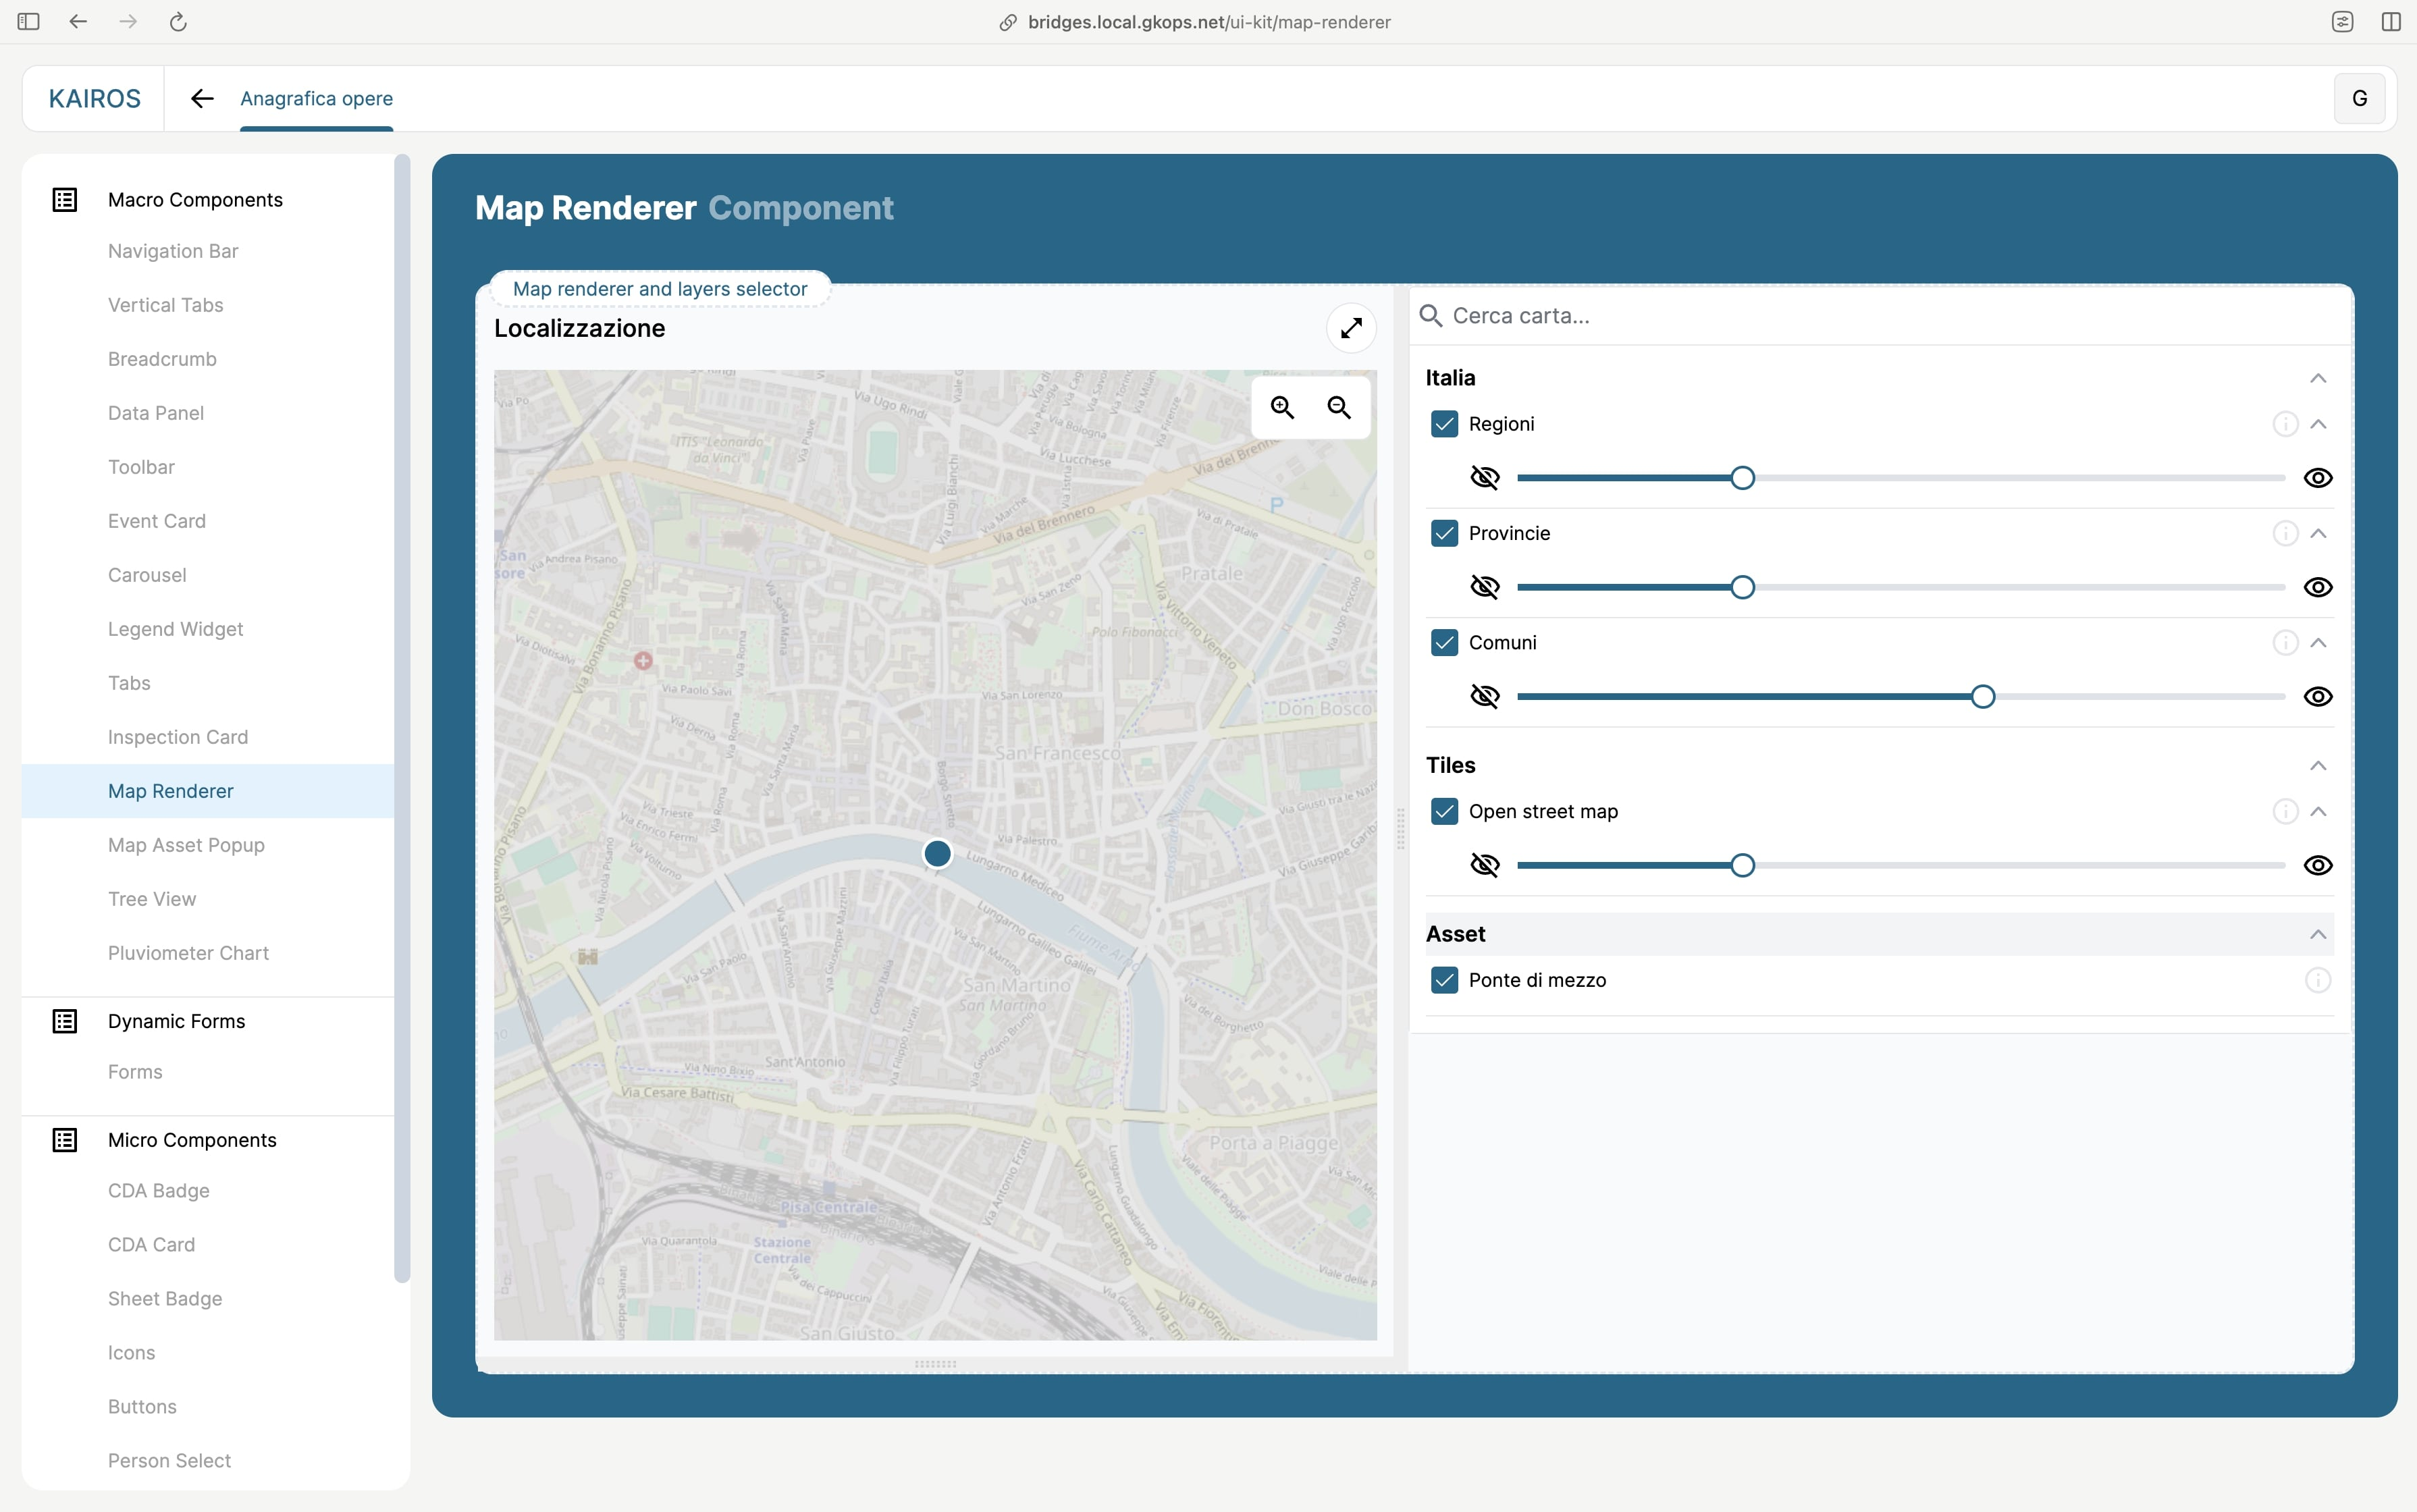
\includegraphics[width=1\textwidth]{Tesi/images/Capitolo4/MapComponent.jpg}
    \caption{Il componente Angular delle mappe nell'Ui-Kit}
    \label{fig:MapComponent}
\end{figure}
\\L'uso dell'Ui-Kit è una pratica comune, specialmente nel contesto di applicazioni Enterprise, in quanto permette agli sviluppatori di poter realizzare tutti i componenti indipendentemente dalla pagina web in cui verranno poi collocati. In questo modo è possibile sia mantenere una coerenza visiva fra tutti i componenti dell'applicazione, aiutando così gli sviluppatori front-end a realizzare un'interfaccia uniforme e coincisa, sia come strumento di presentazione del design ai potenziali clienti, così da fornire loro un'anteprima dell'aspetto e delle funzionalità dell'applicazione.
\\Ovviamente l'uso dell'Ui-Kit è reso possibile grazie ai framework JavaScript come Angular, la cui architettura modulare rende possibile l'esportazione dei componenti creati in altre pagine web dell'applicazione. Ad esempio, quando uno sviluppatore crea un componente nell'Ui-Kit, può facilmente importarlo e utilizzarlo all'interno delle varie pagine del sito, senza doverlo ricreare da zero ogni volta. Senza Angular, questa operazione sarebbe molto più laboriosa, dovendo riscrivere più volte lo stesso codice, e quindi non risulterebbe più conveniente. La prima parte di tirocinio si è quindi dedicata al continuo e all'estensione del componente Angular delle mappe, andando ad implementare le funzionalità precedentemente illustrate.

\subsection*{Censimento delle Mappe}

\\Dopo questa fase di apprendimento iniziale, il candidato ha collaborato con l'azienda per identificare le fonti da cui raccogliere le mappe necessarie, censendole in un documento dettagliato. Questo processo ha permesso di avere una panoramica completa delle risorse geospaziali disponibili e di comprendere come organizzarle e utilizzarle nel contesto del tirocinio. Le mappe utilizzate all'interno del progetto provenivano principalmente da tre fonti:
\begin{itemize}
    \item \textit{Geoportale Nazionale}, un portale gestito dal Ministero dell'Ambiente e della Sicurezza Energetica che contiene dati geospaziali forniti tramite protocollo OGC, quali WMS e WFS. É possibile reperire le mappe utilizzate dal loro sito \cite{GeoPortaleNazionale}.
    \item \textit{IdroGEO}, una piattaforma gestita da ISPRA (Istituto Superiore per la Protezione della Ricerca Ambientale), che permette agli utenti di accedere e di scaricare dati di mappe, in formato Shapefile o GeoJSON, relativi al rischio idrogeologico in Italia. Precisamente fornisce informazioni sull'Inventario dei Fenomeni Franosi in Italia (IFFI) e sulle mappe nazionali di pericolosità da frane e alluvioni e sugli indicatori di rischio associati.
    \item \textit{GeoCart}, un'azienda italiana specializzata nella produzione e distribuzione di mappe e prodotti cartografici \cite{GeoCart}. Anche in questo caso le mappe sono in formato Shapefile, ma a differenza di quelle precedenti, non sono di dominio pubblico e non sono accessibili in modo gratuito. Sono risorse sviluppate ai fini commerciali.
\end{itemize}

\section{Integrazione del formato GeoJSON}

Il candidato, sotto supervisione del tutor aziendale, ha iniziato a contribuire al progetto realizzando una nuova pagina web all'interno dell'applicazione. In questa pagina ha importato il componente Angular delle mappe, originariamente sviluppato dall'azienda, così da poterci integrare successivamente il supporto ai protocolli OGC richiesti e iniziare a testare le mappe censite.
\\Come prima funzionalità, è stato deciso di aggiungere il supporto al formato GeoJSON; questo formato, essendo utilizzato generalmente per i protocolli WFS, non trasporta direttamente un'immagine raster di una mappa, bensì fornisce un insieme di dati che devono essere letti ed interpretati dal client che li richiede. Quindi sarà compito del client, e in questo caso del tirocinante, occuparsi di elaborare questi dati al fine di rappresentarli graficamente a schermo. 
\\Il candidato ha selezionato come prima mappa da testare quella delle frane in Toscana, fornita da IdroGEO, in quanto tutte quelle fornite da questo ente potevano essere scaricate localmente e caricate all'interno del progetto. Tale decisione è stata presa così da semplificare il processo di sviluppo, andando a limitare il più possibile il rischio di errore dovuto ad eventuali problemi di disservizio dei server di mappe esterni. Ad esempio, una mappa fornita dal Geoportale Nazionale tramite servizio WFS potrebbe risultare momentaneamente non disponibile, non riuscendo così a stabilire se il codice scritto fosse corretto o meno.
\\La mappa selezionata conteneva al suo interno una collezione di Feature, dove ciascuna di esse rappresentava una frana avvenuta all'interno della regione. Ogni Feature aveva informazioni:
\begin{itemize}
    \item sul tipo di geometria utilizzata, che in questo caso corrispondeva a un punto;
    \item sulle coordinate geografiche di ciascun punto;
    \item relative ad ogni frana.    
\end{itemize}
Qui di seguito viene riportata una Feature presente all'interno del file JSON della mappa.
\lstinputlisting[language=JSON, caption={Mappa delle frane in Toscana, formato GeoJSON}]{listings/Capitolo4/franeToscana.json}
Lo sviluppo si è concentrato nel modificare le classi \verb|BuildLayer.ts| e \verb|MapModel.ts|, già sviluppate dall'azienda, responsabili di far eseguire ad OpenLayers il rendering della mappa in base al tipo di formato scelto, in quanto ogni formato presentava delle proprietà differenti che dovevano essere gestite in modo appropriato. 
\\Per verificare il funzionamento del codice, il tirocinante ha stilato, all'interno della pagina web, una nuova sezione con cui poter scegliere le varie mappe e ha reso così disponibile quella delle frane. Successivamente ha fatto in modo che la mappa, rappresentata come "layer", venisse sovrapposta a quella di OpenStreetMap, la quale era stata scelta come quella di default all'interno del progetto. In questo modo è stato quindi possibile comprendere se la mappa in formato GeoJSON venisse rappresentata correttamente, in quanto, senza l'uso del layer di default, si sarebbe vista l'immagine della mappa su uno sfondo bianco, non riuscendo così a orientarsi in termini geografici.

\subsection{Risoluzione del problema di proiezione}

\\La prima problematica riscontrata, infatti, è stata quella dell'errata proiezione utilizzata per la rappresentazione della mappa. Quest'ultima utilizzava una proiezione differente rispetto a quella di default posta da OpenLayers, andando così a rappresentare la mappa della Toscana a delle coordinante totalmente differenti rispetto a quelle attese. Precisamente, l'insieme dei punti contenuti all'interno della mappa venivano rappresentati a delle coordinate scritte nella proiezione EPSG:32632 e venivano lette e interpretate da OpenLayers con la proiezione di base EPSG:3857, andando così a collocare l'insieme dei punti in un'area totalmente errata.
\\Per risolvere il problema, il candidato ha prima effettuato uno studio sulla differenza delle due proiezioni e successivamente ha trovato, insieme al tutor aziendale, una libreria nota con il nome di \textit{Proj4}, la quale si occupa principalmente di eseguire le conversioni tra diversi sistemi di coordinate geografiche. In questo modo è stato quindi possibile mantenere la mappa allo stato attuale e far calcolare, a tempo di runtime, la sua nuova proiezione al front-end.
\\Tale libreria, che prende il nome di \textit{Proj4J} per la sua versione di JavaScript, è stata quindi aggiunta al progetto mediante l'utilizzo del gestore di pacchetti Yarn. Dopo averla installata con successo, il tirocinante si è impegnato a comprendere il suo funzionamento e ad includerla nella parte di codice da lui scritta precedentemente. 
\medskip
\\Nel dettaglio, la libreria effettua una trasformazione delle coordinate geografiche partendo dalla proiezione utilizzata dalla mappa interessata (in questo caso EPSG:32632), a quella utilizzata da OpenLayers (EPSG:3857). Per fare ciò, è necessario registrare nel codice un nuovo tipo di proiezione, attraverso la chiamata del metodo \verb|proj4.defs()|, e successivamente, utilizzare la proiezione appena registrata all'interno del codice che si occupa della visualizzazione del layer. In automatico, OpenLayers capirà che quel layer ha una proiezione differente rispetto a quella utilizzata di base e si affiderà a Proj4 per effettuare il cambio di proiezione. 
\\Per definire un nuovo tipo di proiezione, il metodo \verb|proj4.defs()| necessita di due argomenti: il primo, semplicemente, corrisponde al nome della proiezione che si vuole registrare. Il secondo, invece, sono un insieme di parametri, rappresentati sotto forma di stringa, che servono alla libreria per effettuare il calcolo della proiezione. 
\\Ad esempio, nel caso della proiezione EPSG:32632, sarà necessario invocare il metodo nel seguente modo:
\begin{lstlisting}[language=Java]{}
proj4.defs("EPSG:32632","+proj=utm +zone=32 +datum=WGS84 +units=m +no_defs +type=crs");
\end{lstlisting}
Tali parametri vengono reperiti dal seguente sito \cite{ProiezioneESPG3857}, il quale fornisce anche ulteriori informazioni del tipo:
\begin{itemize}
    \item una breve descrizione su come la proiezione viene generalmente utilizzata;
    \item un insieme di proiezioni alternative che possono essere impiegate al posto di quella interessata, utile quando la mappa che si vuole mostrare possiede una proiezione non supportata;
    \item delle proprietà generali sulla proiezione, come l'unità di misura utilizzata, il sistema di coordinate, etc...
    \item una mappa interattiva che mostra il modo in cui la proiezione viene applicata;
\end{itemize}
Ad esempio, nel caso della proiezione EPSG:3857 \cite{ProiezioneESPG3857}, viene spiegato che quest'ultima è usata per rappresentare le mappe come Google Maps, o appunto, OpenStreetMap. Le sue proiezioni alternative sono: 900913, 3587, 54004, 41001, 102113, 102100, 3785; la sua proiezione è definita nel seguente modo:
\begin{lstlisting}[language=Java]{}
proj4.defs("EPSG:3857","+proj=merc +a=6378137 +b=6378137 +lat_ts=0 +lon_0=0 +x_0=0 +y_0=0 +k=1 +units=m +nadgrids=@null +wktext +no_defs +type=crs");
\end{lstlisting}

%\lstinputlisting[language=Java, caption={Implementazione Stili}]{listings/Capitolo4/map model e build layer map.js}

\subsection{Risoluzione del problema di Clustering }

Dopo essere riuscito a mostrare la mappa delle frane nella giusta proiezione, il tirocinante ha riscontrato un ulteriore problema: poiché il file GeoJSON selezionato aveva una dimensione di circa 60MB, la quantità dei punti (corrispondenti alle frane) all'interno del file era troppo elevata per essere visualizzata contemporaneamente da OpenLayers.
\\Al primo tentativo, infatti, il consumo della RAM, utilizzato per mostrare tutti i punti della mappa a schermo, era così elevato a al punto che il programma ha subito un'interruzione anomala, dovuta dalla mancanza di risorse di sistema. Il lavoro del candidato è quindi proseguito cercando una soluzione a tale problema.
\\OpenLayers offre, attraverso le sue API, la possibilità di "clusterizzare" i punti della mappa, cioè permette di raggruppare i punti che sono vicini l'uno all'altro, mostrando a schermo solamente un punto unico. Naturalmente, quando si effettua uno zoom sulla mappa, i cluster si scompongono progressivamente andando così a mostrare i singoli punti contenuti al loro interno. In questo modo, dovendo visualizzare una quantità minore di punti, i consumi di risorse richiesti dall'applicazione sono meno elevati, riuscendo così a visualizzare la mappa correttamente.
\\Per fare ciò, è stato necessario modificare ulteriormente il codice che si occupava della visualizzazione del layer, andando ad aggiungere il meccanismo di clustering offerto dalla libreria stessa. L'uso del clustering richiedeva, da parte dell'utilizzatore, un valore arbitrario che definiva la distanza con cui dovevano essere raggruppati i punti; se la distanza era impostata a zero, il clustering era pressoché inesistente. Dopo aver implementato con successo il meccanismo di clustering, il candidato è finalmente riuscito a mostrare correttamente la mappa a schermo. Si guardi l'immagine \ref{fig:toscanaGeoJSON} per un esempio.
\begin{figure}[htbp]
      \centering
      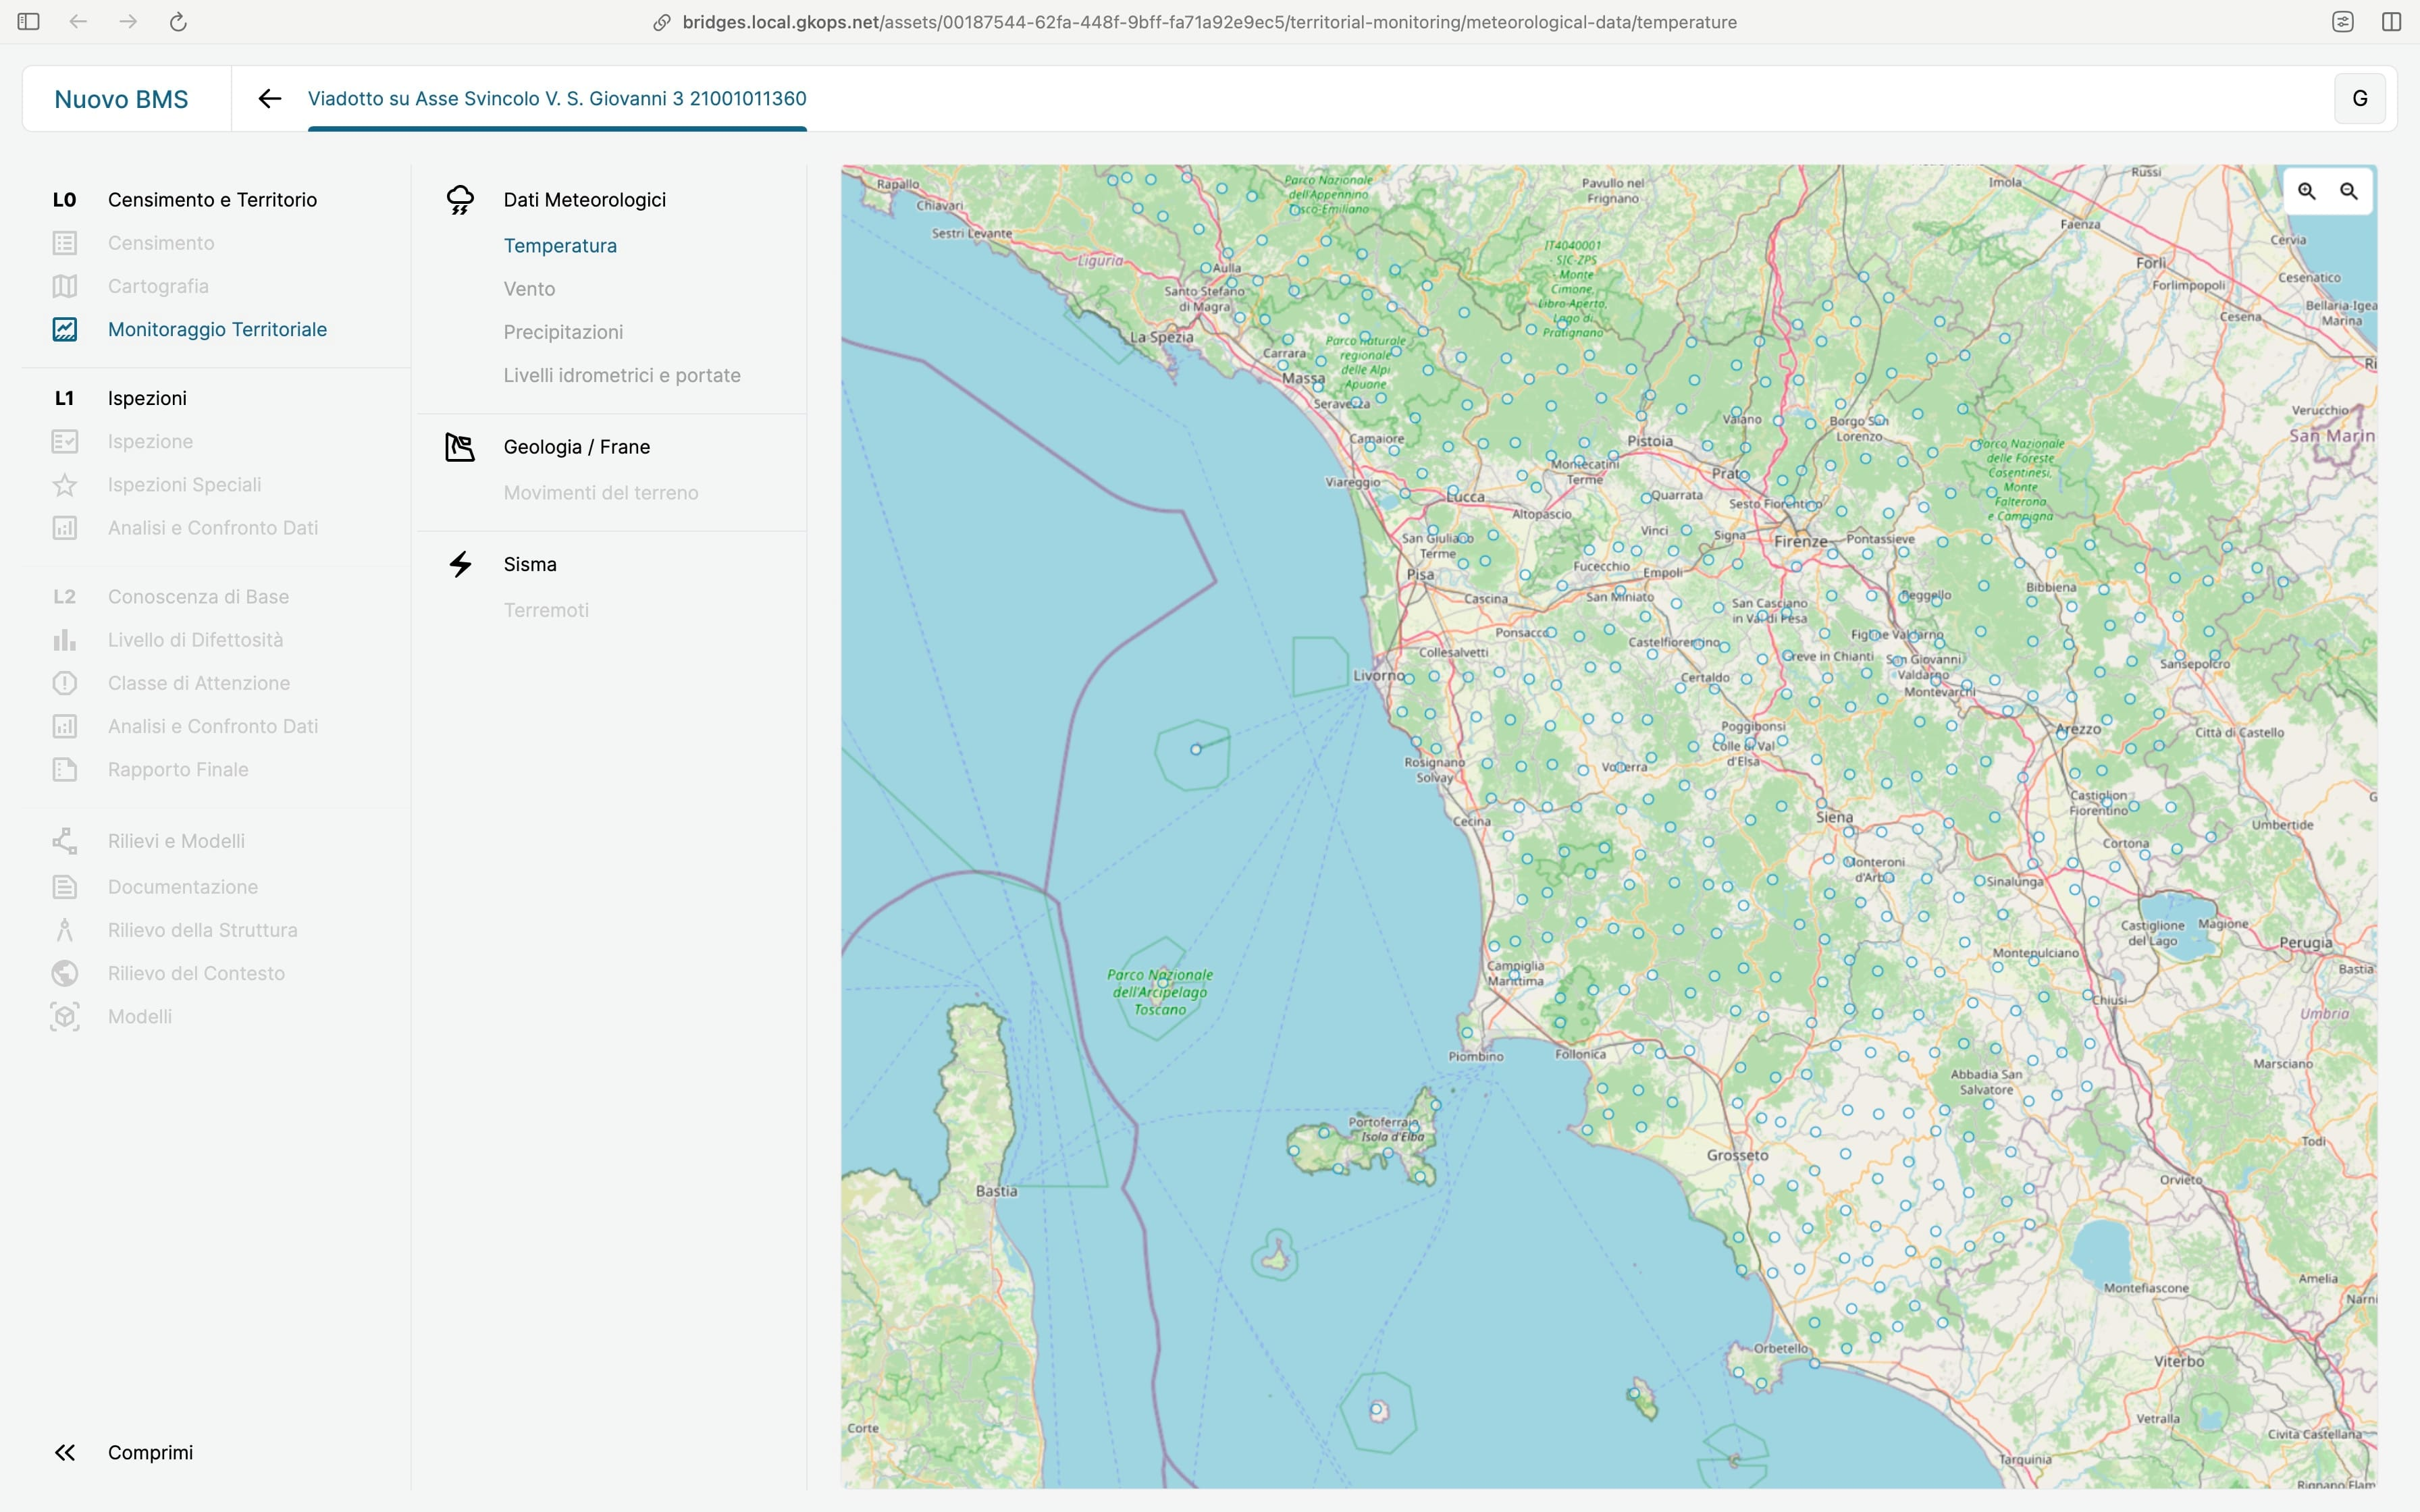
\includegraphics[width=1\textwidth]{Tesi/images/Capitolo4/toscanaGeoJSON.jpg}
      \caption{Mappa delle frane in Toscana, formato GeoJSON}
      \label{fig:toscanaGeoJSON}
\end{figure}

\subsection{Risoluzione del problema di stile con i punti}

Tuttavia, come si può notare dall'immagine \ref{fig:toscanaGeoJSON}, i punti mostrati sulla mappa non erano molto visibili. Inoltre, risultava difficile comprendere se il punto che si stava osservando era un punto di cluster o meno e, nel caso fosse stato un punto di cluster, non era chiaro quanti punti contenesse al suo interno. 
\\Il tirocinante si è quindi occupato di applicare uno stile ai nuovi punti ottenuti, distinguendoli così da quelli appartenenti a "cluster" piuttosto che a "non cluster". Sono stati così realizzati, facendo uso della classe \verb|Style| fornita dalla libreria di OpenLayers, tre stili: il primo si occupa di stilare il punto del cluster, il quale, oltre a renderlo più evidente, include un numero rappresentante i punti contenuti al suo interno. Il secondo, invece, riguarda il singolo punto non cluster, che si mostra come un triangolo rosso, così da essere facilmente visibile rispetto agli altri. L'ultimo, infine, è uno stile che serve a gestire gli errori: viene utilizzato per rappresentare i punti in cui lo stile scelto non viene applicato all'interno della mappa. Per essere subito notato, viene raffigurato come un triangolo giallo con un punto esclamativo al suo interno. Infine, questi stili sono stati poi inseriti all'interno di una nuova classe, nota con il nome di \verb|feature-style.ts|, così da averli organizzati in modo appropriato. Si veda l'immagine \ref{fig:toscanaGeoJSONStyle} per un esempio.
\begin{figure}[htbp]
      \centering
      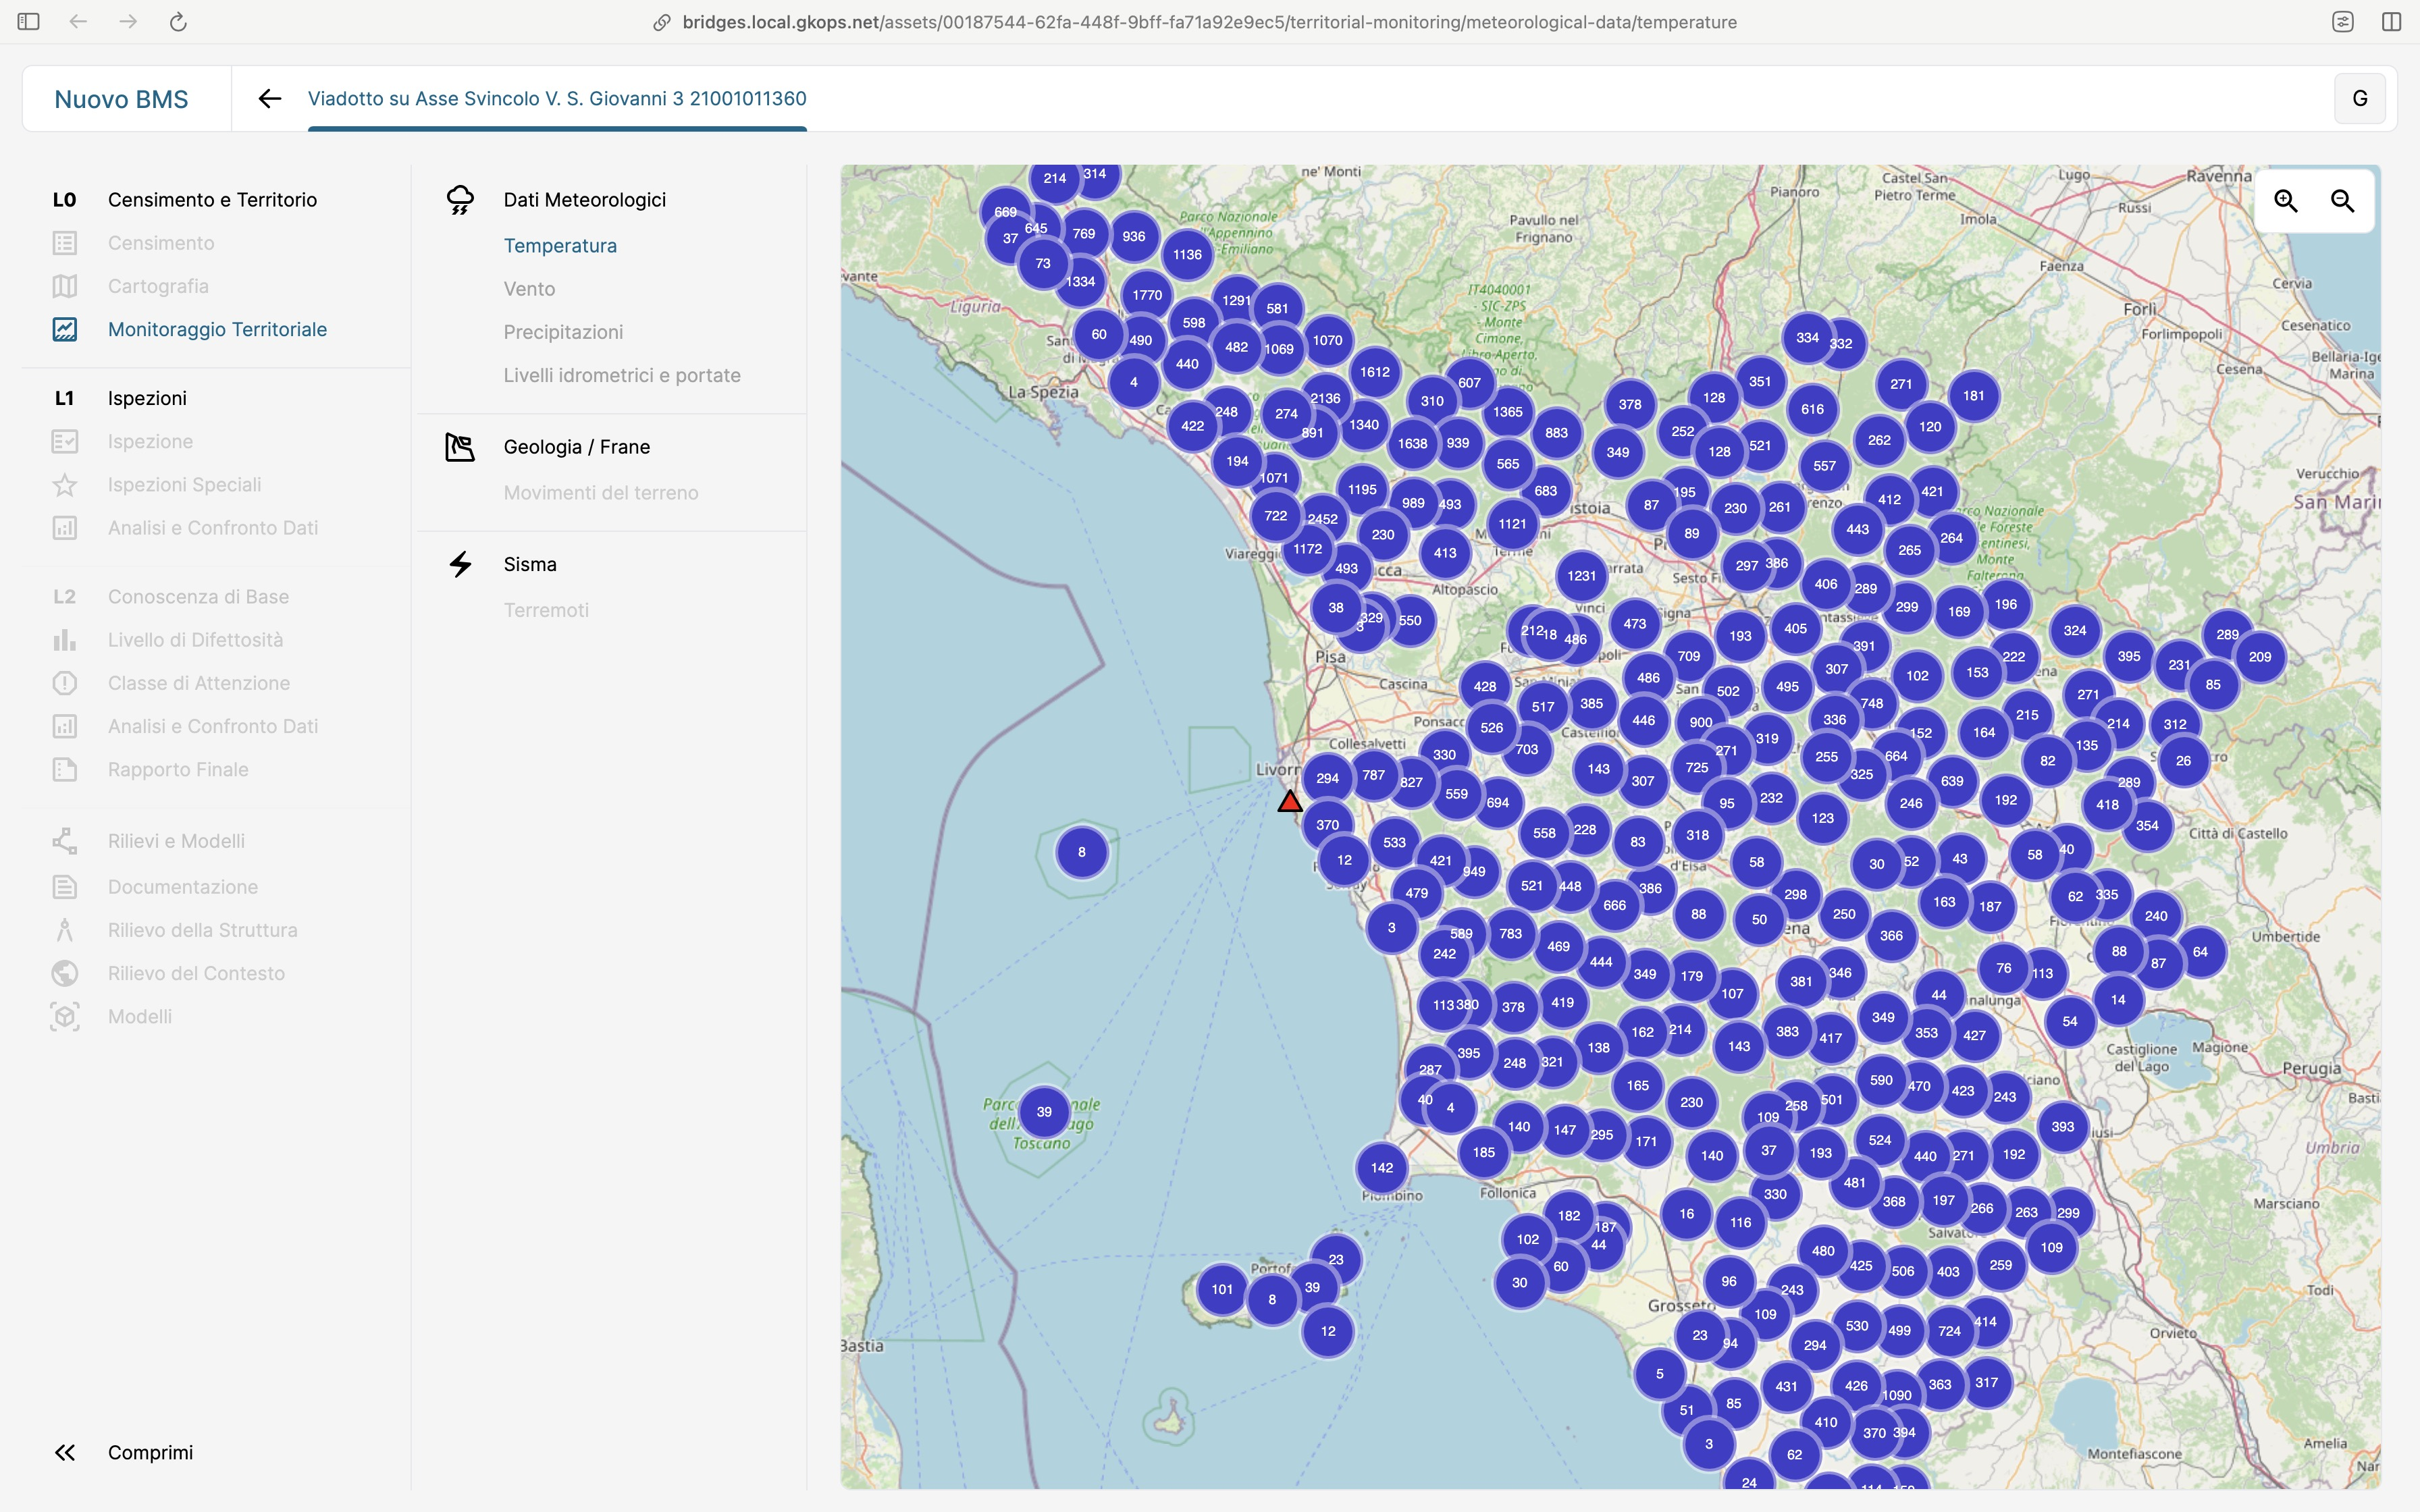
\includegraphics[width=1\textwidth]{Tesi/images/Capitolo4/toscanaGeoJSONStyle.jpeg}
      \caption{Mappa delle frane in Toscana con stile applicato}
      \label{fig:toscanaGeoJSONStyle}
\end{figure}

\subsection{Risoluzione del problema di interazione con i punti}

L'ultimo problema che rimaneva da risolvere era quello di avere un meccanismo che potesse recuperare le informazioni di ogni singola Feature. A tale scopo, il tirocinante ha deciso di aggiungere la possibilità di poter cliccare su ogni punto mostrato sulla mappa. Nel dettaglio, si è fatto in modo che, al click di un utente su un punto, venisse mostrata una finestra, sempre in primo piano rispetto alla mappa sottostante, contenente le informazioni relative al punto selezionato.
\\Per fare ciò, è stato sufficiente registrare una nuova funzione sull'evento di click della Feature. Questa funzione si occupa di recuperare l'ID del punto cliccato e, successivamente, di individuare all'interno della lista di feature quella con l'ID corrispondente a quella appena ottenuta. Una volta recuperata, basta leggere il contenuto del campo "properties" al suo interno e mostrarlo a schermo nella finestra creata.
\\Tuttavia, i punti, essendo alcuni di loro dei cluster, non contengono direttamente al loro interno le informazioni della frana, peranto è stato necessario distinguere nuovamente un punto di "cluster" da uno "non cluster". Per fare ciò, è stato necessario aggiungere un controllo che si attiva quando l'utente clicca su un punto: se questo contiene al suo interno più elementi, allora si tratta di un cluster, mostrando nella finestra il numero di punti che contiene al suo interno. Altrimenti, se il punto interessato contiene un solo elemento, allora si tratta di una frana.
\\Il tirocinante ha infine implementato due diverse modalità di gestione del click: una in cui la schermata rimane aperta e si chiude solo se si clicca su un altro punto e l'altra che consente di avere più finestre aperte cliccando sui vari punti, permettendo così di confrontarli tra loro. Si veda l'immagine \ref{fig:toscanaClickGeoJSON} per un esempio.
\begin{figure}[htbp]
      \centering
      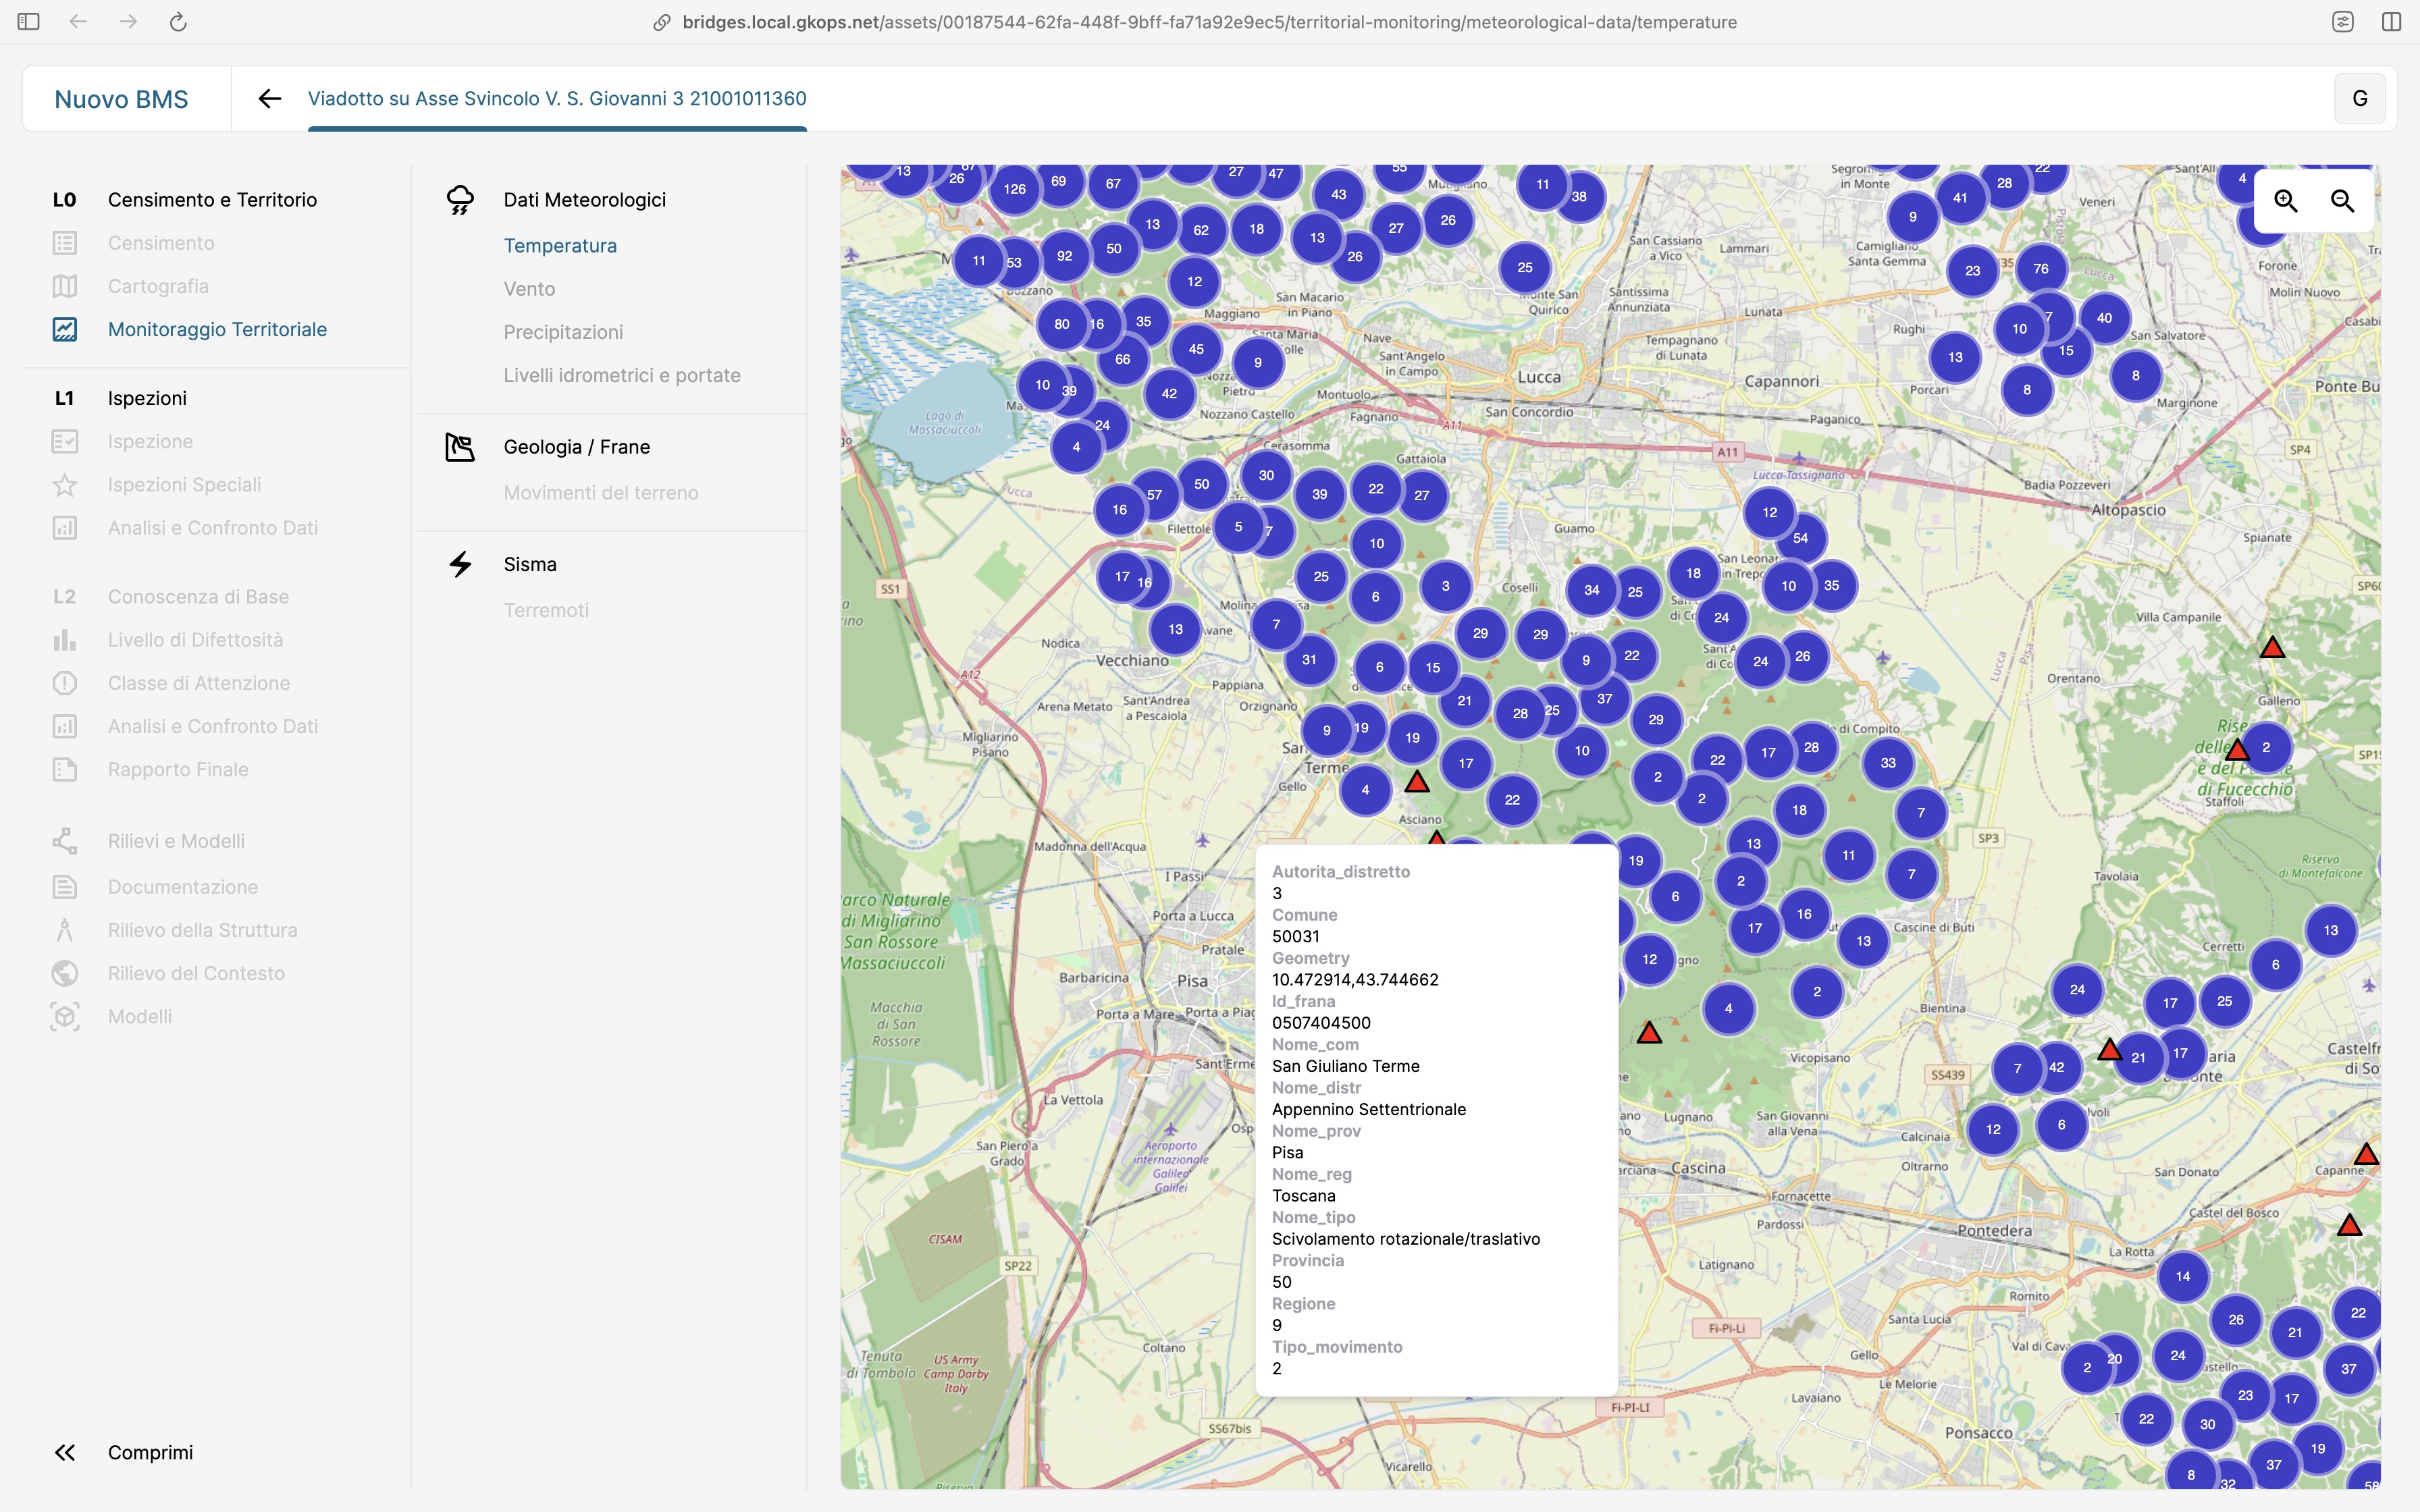
\includegraphics[width=1\textwidth]{Tesi/images/Capitolo4/toscanaClickGeoJSON.jpeg}
      \caption{Mappa delle frane in Toscana, informazioni della frana a schermo}
      \label{fig:toscanaClickGeoJSON}
\end{figure}

\subsection{Considerazioni sul risultato ottenuto}

Sebbene la mappa risultasse funzionante, in questo tipo di implementazione persistevano comunque dei problemi che non potevano essere trascurati. Il primo risiedeva nel fatto che, in quel momento, il file JSON della mappa era incluso direttamente all'interno del progetto; questo approccio potrebbe essere accettabile per scopi di debug o test, ma non poteva essere mantenuto in modo permanente: caricare centinaia di mappe direttamente nel front-end è inefficiente e sopratutto difficile da gestire. 
\\Un altro problema era che, fino ad allora, non era stato sviluppato alcun meccanismo che si occupasse di gestire l'inserimento di mappe in maniera dinamica. Infatti, la mappa era stata inserita in maniera "hard coded",  cioè nel codice era specificato esplicitamente quale mappa utilizzare, non permettendo quindi di supportare eventuali nuove mappe.
\\Inoltre, questa pratica consumava molte risorse, dato che il calcolo dei punti e delle proiezioni veniva eseguito direttamente dal front-end. Sarebbe quindi opportuno creare una figura, lato back-end, che si occupi dove possibile di eseguire direttamente il cambio di proiezione e fornire i dati calcolati al client. 
\\Infine, risultava difficile sviluppare un sistema che permettesse di limitare o manipolare la quantità di punti da caricare, in quanto il front-end era obbligato a leggere l'intero file JSON per eseguire questo tipo di operazioni.

\section{Integrazione del protocollo WMS}

Il tirocinante ha poi proseguito con l'implementazione del supporto al protocollo WMS. Tale protocollo è stato scelto come primo da integrare, in quanto è stato ritenuto dal candidato il più agevole rispetto agli altri standard. Questo è da ricercarsi nel fatto che il protocollo WMS, restituendo direttamente l'immagine di una mappa, non richiede di dover gestire la complessità delle tiles (come nel WMTS) o di dover rappresentare graficamente i dati ricevuti (come nel WFS).
\\Tuttavia, al contrario dell'implementazione precedente, non c'era più la possibilità di scaricare i dati di una mappa localmente ed inserirli all'interno del progetto, ma era obbligatorio reperire le immagini della mappa da un server esterno. Per fare ciò, quindi, era necessario realizzare un meccanismo che fosse in grado di effettuare una serie di richieste HTTP ad un server WMS, così da ricevere l'intera immagine della mappa e successivamente mostrarla a schermo nella giusta proiezione. Il tirocinante ha scelto, come prima mappa da integrare, la "Carta ecopedologica d'Italia" (figura \ref{fig:italiaWMS}), fornita da un server esterno del Geoportale Nazionale.
\\Il lavoro è quindi cominciato modificando ulteriormente le classi \verb|BuildLayer.ts| e \verb|MapModel.ts|, aggiungendo il supporto al protocollo WMS mediante l'uso della libreria di OpenLayers. Precisamente, si è fatto uso delle delle classi \verb|ImageWMS| e \verb|WMSCapabilities|, in quanto, come già spiegato, consentivano di eseguire le richieste HTTP al server WMS, senza doversi preoccupare di farle manualmente o di analizzare il contenuto delle loro risposte.
\\Il codice così scritto iniziava con una richiesta di GetCapabilities fatta al server del Geoportale Nazionale. Dopo aver ottenuto una risposta, veniva eseguito un parser, utilizzando la classe \verb|WMSCapabilities|, così da ottenere la lista di tutti i layer disponili con le rispettive proiezioni. Come risposta, il server forniva due layer accessibili: il primo, denominato "Carta ecopedologica - Generale" e il secondo "Carta ecopedologica - Dettaglio", entrambi disponibili in molte proiezioni, tra cui quella utilizzata da OpenLayers. Ciò ha implicato che, a differenza della mappa in GeoJSON precedentemente implementata, non era necessario eseguire il calcolo per effettuare il cambio di proiezione con Proj4.
\\Dopo aver scelto come primo layer da visualizzare "Carta ecopedologica - Generale", è stato sufficiente utilizzare la classe \verb|ImageWMS| che, passando il layer come parametro, ha eseguito automaticamente la richiesta GetMap al server, senza doversi preoccupare di inserire manualmente i query params corretti (come CRS, BBOX, FORMAT, etc...) per ricevere l'immagine della mappa.
\\Il lavoro del candidato è poi continuato aggiungendo alla sezione precedentemente sviluppata la nuova mappa disponibile, potendo così verificare se il codice da lui scritto fosse funzionante o meno.

\subsection{Caricamenti lenti e Rate Limiting}

La prima problematica riscontrata riguardava la lentezza delle risposte HTTP inviate dal server WMS per ottenere le immagini, causando notevoli ritardi nel caricamento della mappa selezionata.
\\Questo problema dipendeva sia dalla lentezza intrinseca dei loro server, sia dalla dimensione dell'immagine richiesta: essendo inviata tramite protocollo WMS, l'immagine non veniva divisa in tiles come in altri protocolli, ma veniva trasmessa attraverso una singola richiesta HTTP con l'intera immagine al suo interno, rendendo quindi più pesante il carico di ogni richiesta. In aggiunta, ogni volta che la telecamera veniva spostata, si effettuava nuovamente una richiesta al server per ricevere la nuova immagine, anche se questa poteva includere porzioni di mappa già presenti nella richiesta precedente.
\\Inoltre, dopo una serie di tentativi e varie richieste HTTP inviate allo stesso servizio, il server WMS del GeoPortale Nazionale ha iniziato a effettuare rate-limiting, cioè ha limitato il numero di richieste che potevano essere inviate in un determinato periodo di tempo, rendendo quindi la mappa non più accessibile.
\\Per ottenere comunque un risultato, è stato necessario limitare il più possibile il numero di richieste da inviare, evitando quindi di spostare troppo la telecamera della mappa per non generarne di nuove. 

\subsection{Considerazioni sul risultato ottenuto}

Sebbene la mappa venisse visualizzata correttamente e nella giusta proiezione, questo tipo di implementazione non era sostenibile a causa dei caricamenti lenti e del rate-limiting imposto dal server. 
\\Inoltre, similmente alla mappa in formato GeoJSON, il codice realizzato era progettato per funzionare esclusivamente con i suoi due rispettivi layer, senza possedere una struttura predisposta a supportare dinamicamente l'aggiunta di mappe ulteriori. In aggiunta, poiché la mappa veniva fornita con la stessa proiezione scelta da OpenLayers, non era stato implementato un sistema per gestire il cambio di proiezione come fatto precedentemente. Ciò poteva risultare un problema nel caso in cui altre mappe venissero fornite con una proiezione diversa, rendendo quindi necessaria un'adeguata gestione delle proiezioni per garantire la loro corretta visualizzazione.
\\Infine, tale sistema non garantiva l'affidabilità del servizio: se la mappa ospitata dai server veniva spostata, eliminata o se il server stesso diventava inattivo o soggetto a manutenzione, l'accesso alla mappa mediante l'applicazione veniva compromesso.
\\Quindi anche in questo caso, era necessario creare una figura esterna, situata all'interno del back-end, che si occupasse di risolvere principalmente queste complicazioni. 
\begin{figure}[htbp]
      \centering
      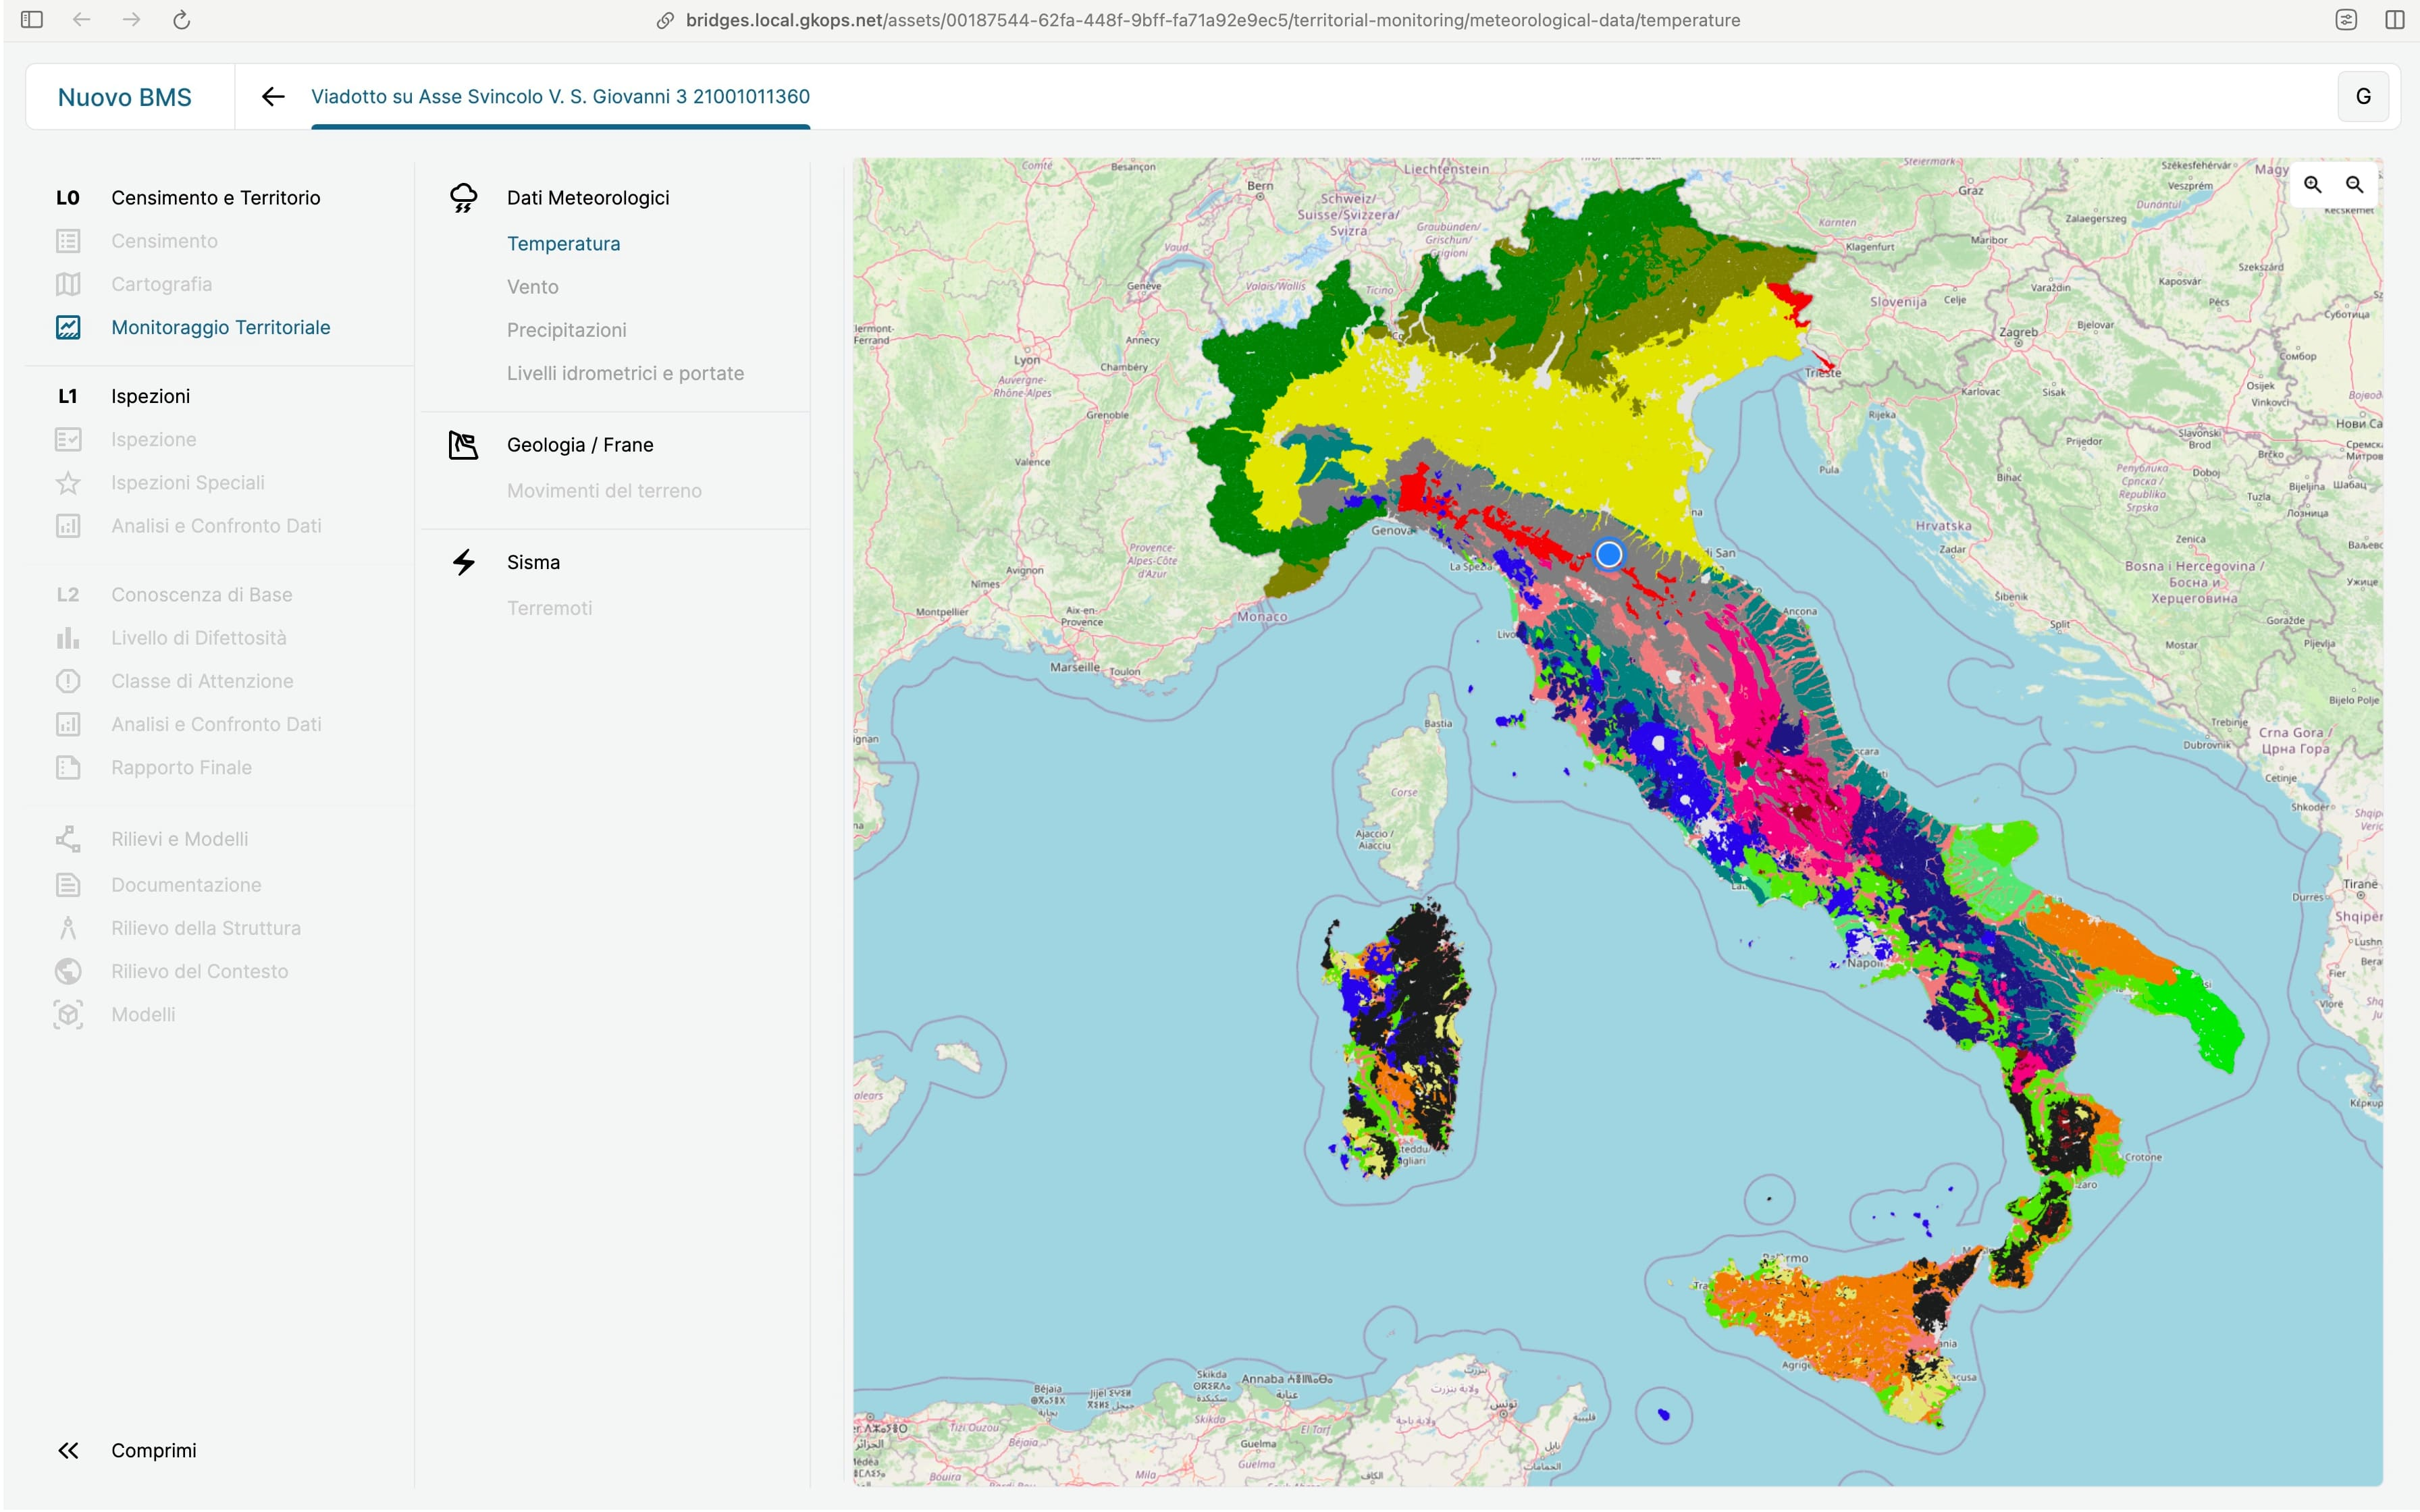
\includegraphics[width=1\textwidth]{Tesi/images/Capitolo4/italiaWMS.jpg}
      \caption{Carta ecopedologica - Generale, protocollo WMS}
      \label{fig:italiaWMS}
\end{figure}

%\lstinputlisting[language=Java, caption={Implementazione BuildLayer}]{listings/Capitolo4/buildLayer.js}
\chapter{Sviluppo Back-end con GeoServer}
\label{cap:chapter5}

\section{Soluzione al problema}

La prima soluzione ideata dal candidato è stata quella di realizzare un server, proprietario dell'azienda, in cui scaricare al suo interno tutte le mappe interessate. L'idea prevedeva la realizzazione di un programma in grado di contattare uno ad uno tutti i server WMS esterni, e scaricare all'interno del server aziendale tutte le mappe disponibili, rispettando ovviamente eventuali rate-limiting imposti. In questo modo, si sarebbero evitati potenziali problemi legati alla latenza dei server e alla possibilità che un servizio diventasse improvvisamente non disponibile.
\\Il problema in questo tipo di implementazione è che il peso delle mappe è estremamente elevato, rendendo quindi molto dispendioso, sia in termini di risorse di calcolo che economiche, realizzare una piattaforma di questo genere. 
\\Innanzitutto, va considerato che non tutte le mappe WMS sono ospitate sugli stessi server; alcuni di essi potrebbero offrire prestazioni migliori e addirittura non applicare alcun tipo di limitazione sulla frequenza delle richieste. In aggiunta, non tutte le mappe richieste dall'applicazione hanno la stessa importanza: potrebbe accadere che alcune mappe vengano frequentemente consultate dagli utenti, mentre altre siano utilizzate raramente, causando un consumo inutile di spazio e risorse. 
\\Inoltre, è importante anche considerare che i server WMS potrebbero aggiungere dei nuovi layer alla richiesta di GetCapabilities in futuro; questo richiederebbe non solo la creazione di un meccanismo per copiare tutte le mappe, ma anche di mantenerle sincronizzate costantemente. Oppure, se in futuro si dovesse aggiungere un nuovo servizio all'interno del programma, risulterebbe laborioso aggiungere manualmente un nuovo server da cui reperire le mappe desiderate, tenendo in considerazione che non tutti i server potrebbero offrire le mappe nello stesso modo. Infatti, come già mostrato, OpenLayers utilizza il campo \verb|serverType| per cambiare il modo in cui esegue le richieste sui vari server di mappe.
\\Infine, poiché la piattaforma è destinata alla commercializzazione, è essenziale considerare l'origine delle mappe: non tutte le mappe sono disponibili con termini di utilizzo che consentono di poterle scaricare e usare gratuitamente a fini commerciali. Alcune richiedono un contatto diretto con i loro server e non offrono legalmente la possibilità di poter scaricare le mappe.
\\Questo non esclude la possibilità che questo tipo di implementazione possa essere sviluppata in futuro, magari limitandola solo alle mappe di maggiore importanza o a quelle che frequentemente presentano problematiche di funzionamento, rendendole quindi inutilizzabili.
\\~\\
Una soluzione più semplice da adottare consisterebbe nell'implementare un meccanismo che si occupi di fare "proxying" dei server esterni, cioè ogniqualvolta che il front-end richiede una mappa, anziché contattare direttamente il server WMS interessato, l'applicazione potrebbe contattare un nostro servizio intermedio. Quest'ultimo, a sua volta, inoltrerebbe la richiesta al server WMS esterno e restituirebbe la risposta al front-end. 
\\Attraverso un meccanismo di questo tipo, sarebbe possibile implementare un sistema di caching delle risposte ottenute dai server WMS esterni: quando il nostro servizio intermedio riceve una richiesta di mappa dal front-end, può verificare se questa è già presente nella cache. Se lo è e non è stata invalidata, il servizio può restituirla  senza dover contattare nuovamente il server esterno.
\\Inoltre, se il programma fosse eseguito all'interno di un WebServer, si avrebbe l'opportunità di sfruttare ulteriori meccanismi di caching: il WebServer potrebbe essere configurato per memorizzare nella sua cache le risposte alle richieste già effettuate al servizio intermedio. Ciò significa che se il client contattasse il WebServer per ricevere una mappa, questo potrebbe direttamente restituirla senza comunicare con il sistema precedentemente citato.
\\Un meccanismo di questo tipo, inoltre, adotterebbe un approccio centralizzato, permettendo ai client di interagire esclusivamente con un unico servizio, semplificando così anche il processo di gestione delle richieste. In questo modo, il modello potrebbe essere esteso per includere anche altri protocolli, come ad esempio il WFS.
\\Questa soluzione non solo affronterebbe il problema del rate-limiting e della lentezza dei server esterni, ma risolverebbe anche le preoccupazioni legate ai termini di utilizzo delle mappe spiegati precedentemente.
\\In conclusione, tale implementazione potrebbe anche essere estesa, andando a realizzare un sistema che permetta di sfruttare altri protocolli più efficienti rispetto allo standard WMS. Ad esempio, si potrebbe realizzare un sistema che, dopo aver ricevuto la risposta dal server WMS esterno, potrebbe convertire l'immagine suddividendola in tiles, per poi restituirle al client tramite protocollo WMTS. Tale meccanismo, già realizzato da altri, prende il nome di GeoServer.

\section{Introduzione a GeoServer}

GeoServer è un software OpenSource scritto in Java che permette di caricare e servire dati di mappe geospaziali.
All'interno di questo programma i dati possono essere caricati in vari formati (come Shapefile, GeoPackage, etc...) per poi essere esposti attraverso l'utilizzo di protocolli standard OGC (come WMS, WMTS, WFS, etc...), oppure attraverso l'utilizzo di altri protocolli come TMS.
Ad esempio, è possibile caricare un file di mappa in formato Shapefile ed esporlo sul proprio server mediante un servizio WMS.
In questo modo un client che supporta tale protocollo, come appunto OpenLayers, può visualizzare la mappa interessata e richiederla in un formato raster come PNG, JPG o simili.

\subsection{Caratteristiche principali}

Come già accennato, una delle funzionalità principali del GeoServer è il "proxying" di servizi OGC, ovvero consente di replicare e mantenere aggiornati i servizi di mappe forniti da server esterni.
\\Ciò è possibile in quanto il GeoServer è in grado di memorizzare al suo interno l'URL che rappresenta la richiesta di GetCapabilities. Come già spiegato, questa richiesta è essenziale per ottenere tutte le informazioni necessarie (layer di mappe, proiezioni, formati, etc...) al fine di richiedere le mappe fornite dal server esterno.
\\In pratica, ogni volta che un client richiede al GeoServer una mappa che non è presente localmente, il GeoServer inizia contattando il server esterno tramite una richiesta di GetCapabilities. Una volta ricevuta la risposta, il GeoServer esegue un'altra richiesta (ad esempio una GetMap nel caso dei servizi WMS) per ottenere la mappa specifica richiesta dal client. Una volta che il GeoServer riceve i dati della mappa dal server esterno, li invia al client come risposta alla sua richiesta originale.
\\Questo consente di memorizzare tutti i dati delle mappe, potenzialmente anche esposte medianti protocolli diversi, sotto un unico server. Tale pratica non solo semplifica la gestione e la manutenzione dei dati geospaziali, ma dal punto di vista del client, viene offerta l'illusione di avere un sistema centralizzato, in cui tutte le mappe sono contenute direttamente sotto un unico servizio.
\\Un'altra importante funzionalità di GeoServer è la capacità di esporre dati geospaziali utilizzando protocolli diversi. 
Ad esempio, è possibile registrare un server esterno di mappe WMS nel modo spiegato precedentemente e successivamente, attraverso GeoServer, renderlo disponibile al client nei protocolli WMS, WMTS, TMS, etc... Questo perché, dal punto di vista del client, la comunicazione avviene col GeoServer, che maschera qualsiasi eventuale ulteriore comunicazione con server esterni. In questo caso, GeoServer si occuperà in automatico di fornire i dati della mappa in tiles, nonostante il servizio esterno non supportasse tale protocollo.

\subsection{Meccanismi di Caching}

Avere tutte le mappe centralizzate sotto un unico server favorisce anche l'utilizzo di meccanismi di caching: a livello di WebServer, per esempio, tramite l'utilizzo di un Reverse Proxy, è possibile configurare politiche di caching per memorizzare temporaneamente le risposte alle richieste HTTP inviate al GeoServer. Questo consente di ridurre il carico su di esso, in quanto alcune richieste possono essere soddisfatte direttamente dalla cache del WebServer senza doverle inoltrare nuovamente al GeoServer. Tale pratica risulterebbe più complessa da fare, se le mappe fossero decentralizzate su servizi esterni, specialmente se di terze parti.
\\Inoltre, GeoServer stesso offre diversi livelli di caching. È possibile infatti configurarlo per memorizzare in una sua cache interna le risposte alle richieste di mappe.
\\Esiste anche la possibilità di memorizzare nella cache la risposta ottenuta dalla richiesta GetCapabilities inviata ai servizi OGC esterni, in modo da evitarne il recupero ogni volta. Questo risulta utile soprattutto quando si ha a che fare con mappe geospaziali che cambiano raramente nel tempo o che non cambiano affatto, anche se è possibile comunque risolvere il problema in parte mettendo una cache di durata più breve. Questo consente a GeoServer di rispondere più rapidamente alle richieste di mappe, utilizzando i dati già memorizzati nella cache anziché elaborarli nuovamente, riducendo così il carico e migliorando i tempi di risposta.

\subsection{Funzionamento di GeoServer}

Geoserver supporta diversi tipi formati e servizi geospaziali, i più noti sono:

\begin{itemize}
      \item Servizi di mappe: WMS, WMTS, WFS, TMS per i servizi di mappe;
      \item Dati raster: GeoPackage, ArcGrid, GeoTIFF, ImageMosaic, WorldImage;
      \item Dati vettoriali o a oggetti geospaziali: ShapeFiles, GeoPackage, PostGIS;
\end{itemize}
Questi ultimi possono essere caricati e gestiti tramite l'utilizzo di un'interfaccia grafica, realizzata sotto forma di un'applicazione web, oppure tramite l'utilizzo di chiamate ad una REST API.
\\Al fine di poter caricare correttamente una mappa all'interno di GeoServer, è necessario creare tre componenti basilari:
\begin{itemize}
      \item Workspace: rappresenta precisamente "l'area di lavoro", cioè il luogo in cui tutte le mappe vengono effettivamente caricate, quest'ultime a sua volta vengono organizzate in all'interno di Storage. Una workspace può contenere uno o più Storage.
      \item Storage: rappresenta il contenitore di mappe che si vuole caricare all'interno di GeoServer. Può essere un servizio WMS, WMTS, WFS, o un dato geospaziale come Shapefile, GeoTIFF, etc... Ovviamente in base al tipo di Storage che si va a creare, le impostazioni visualizzate sull'interfaccia grafica (o i query params da inviare secondo la REST API) saranno differenti. Per esempio, se si va a creare un servizio esterno WMS, sarà chiesto il link delle capabilities da contattare. Se si andrà a caricare uno Shapefile, sarà richiesto il percorso locale in cui il file si trova.
      \item Layer: rappresenta la mappa effettiva, quella che verrà poi fornita al Front-end. È ciò che restituisce lo storage una volta ricevuta la risposta alla GetCapabilities, nel caso di un servizio OGC, o ciò che contiene uno Shapefile. Ovviamente più layer possono stare all'interno di uno storage.
\end{itemize}
Dal punto di vista di architetturale, come si può vedere dal codice fornito su GitHub [7], GeoServer è stato sviluppato in Java utilizzando Spring come Framework, mentre l’interfaccia grafica è stata realizzata con Wicket. Infine, la REST API è stata anch'essa implementata utilizzando Spring, precisamente con Spring MVC Framework.
\\Una nota importante riguardo la REST API è che, come verrà spiegato più dettagliatamente in seguito, la specifica fornita da GeoServer stesso presenta delle carenze in termini di usabilità e affidabilità: tale specifica, infatti, non è stata più aggiornata con le continue evoluzioni di GeoServer, andando a così a compromettere il suo funzionamento. L'uso delle API di GeoServer è stata una parte integrante del tirocinio e ciò ha complicato notevolmente il suo utilizzo.

\section{Integrazione di GeoServer nel progetto}

Il tirocinio è proseguito con l'installazione del software GeoServer all'interno dell'applicazione. Per garantire una gestione agevole e una configurazione uniforme dell'ambiente di sviluppo, è stato deciso di adottare un'immagine Docker per l'installazione di questo software.
\\Inizialmente, è stata scelta l'immagine Docker ufficiale di GeoServer, fornita direttamente dalla loro pagina GitHub, che è stata installata seguendo il processo di installazione descritto nella loro documentazione.  
Successivamente, poiché tale immagine non supportava l'architettura ARM, la quale era necessaria per esigenze di sviluppo del progetto, è stata adottata una immagine diversa, non ufficiale, presente sempre su GitHub al seguente indirizzo \cite{ImmagineGithubGeoServer}.
\\Per effettuare questa operazione, è stato necessario apportare delle modifiche ai file di configurazione Docker già esistenti nel progetto: inizialmente, è stata aggiunta l'immagine di GeoServer selezionata al file  \verb|compose.yaml| e successivamente, è stato necessario intervenire sul file \verb|compose.override.yaml| per modificare la porta di GeoServer da 8080 a 8888, rendendolo così accessibile, in quanto la porta 8080 era già occupata da un altro servizio.
\\Infine, per rendere disponibile il servizio di GeoServer ad un indirizzo diverso da quello locale (127.0.0.1:8888), è stato configurato il reverse proxy di Caddy in modo da ottenere un dominio con certificazione TLS installata, il quale reindirizzava  direttamente al servizio di GeoServer stesso. 

\subsection{Problematiche riscontrate}

Dopo aver installato con successo l'immagine di Docker, è stato riscontrato un problema relativo alla persistenza dei file generati da GeoServer. Precisamente, all'avvio dell'applicazione all'interno di un container Docker, il GeoServer generava una serie di file in una directory specifica, i quali erano essenziali per il funzionamento dell'applicazione stessa e per mantenere le configurazioni impostate. In aggiunta, ogni volta che venivano caricate delle mappe al suo interno, il GeoServer generava dei file ulteriori per tenere traccia delle mappe appena inserite, anch'essi sempre presenti nello stesso percorso.
% non riesco a dire che quando si modificano delle impostazioni più specifiche si generavano dei nuovi file 
\\Il problema si manifestava quando il container di Docker veniva arrestato, comportando la cancellazione di tutti i dati al suo interno, inclusi i file di configurazione e delle mappe appena menzionati. Di conseguenza, non solo ogni volta che si avviava il container le configurazioni di GeoServer si resettavano, ma le mappe inserite andavano perse.
\\Per risolvere questo problema, è stata implementata una soluzione che utilizza i volumi forniti da Docker stesso, i quali consentono di memorizzare i dati in modo persistente anche dopo la terminazione del container.
\\Infine, per garantire l'accesso alle mappe di GeoCart e di IdroGEO, precedentemente caricate su un drive aziendale di Google, è stato utilizzato Rclone, un software che permette la creazione di cartelle o dischi virtuali collegati ai servizi Cloud. 
\\Precisamente, è stato realizzato uno script in bash che, attraverso l'uso del comando \verb|rclone sync|, scarica automaticamente le mappe dal drive aziendale e le inserisce in una specifica cartella collegata al volume del container di Docker. Grazie a questa configurazione, le mappe venivano così mantenute sincronizzate. La configurazione finale di Docker ottenuta è quindi la seguente:

\begin{lstlisting}[language=Java]{}
  geoserver:
    image: kartoza/geoserver:2.24.2
    environment:
      - GEOSERVER_CSRF_DISABLED=true
      - GEOSERVER_ADMIN_PASSWORD=geoserver
      - GEOSERVER_ADMIN_USER=admin
    restart: unless-stopped
    ports:
      - "8888:8080"
    volumes:
      - ./workspaces/geoserver/scripts/chown-data.sh:/docker-entrypoint-geoserver.d/chown-data.sh
      - ./workspaces/geoserver/data:/opt/geoserver/data_dir
      - ./workspaces/geoserver/layers:/opt/layers
\end{lstlisting}

\section{Integrazione delle mappe con GeoServer}

Il candidato ha proseguito il proprio lavoro studiando il funzionamento di tale software, attraverso la documentazione ufficiale \cite{DocumentazioneGeoServer}. Successivamente, utilizzando l'interfaccia grafica fornita da GeoServer stesso, ha poi iniziato ad interagire con l'applicazione, così da comprendere appieno le funzionalità che offriva. Il tirocinante ha cominciato inserendo alcune mappe all'interno di GeoServer, avviando così una serie di test per valutare la sua operatività e analizzare le prestazioni effettive dell'applicazione.

\subsection{Implementazione protocollo WMS}

\\La prima prova si è concentrata sulle mappe WMS, con l'obbiettivo di valutare il loro comportamento all'interno di GeoServer rispetto alla sua assenza, cercando quindi di comprendere se l'utilizzo di tale software, come server di mappe, influenzasse in qualche modo le prestazioni complessive.
\\Per fare ciò, è stata creata una Workspace al cui interno sono stati inseriti degli Storage. Ognuno di essi, a sua volta, è stato poi configurato per effettuare proxying verso un server WMS esterno. Infine, per ogni Storage, sono stati caricati tutti i layer che vi erano associati, rendendoli così disponibili a trasmettere le immagini di mappa tramite protocollo WMS. Le mappe considerate in questa operazione sono state: la "Carta ecopedologica d’Italia", ovvero la stessa utilizzata precedentemente, in modo da avere un confronto fra le due implementazioni e la carta "Alluvioni - Estensione dell'area allagabile (PGRA 2021)" \ref{fig:italiaAlluvioni}, selezionata per testare una nuova mappa.
\\Il lavoro è poi continuato con la modifica del codice front-end sviluppato in precedenza, cambiando l'indirizzo a cui il client si collegava per recuperare i dati delle mappe. La differenza in questa operazione è stata che, grazie al GeoServer, le mappe potevano essere recuperate attraverso due tipi di richieste GetCapabilities. La prima richiesta, più generale, restituiva la lista di tutti i layer disponibili, indipendentemente dalla Workspace in cui si trovavano. La seconda, invece, conteneva singolarmente la lista di mappe di ogni Workspace, rivelandosi utile per ridurre il peso di ogni richiesta.
\\Per semplificare questa fase di test, è stata scelta la prima opzione nonostante fosse meno efficiente, in quanto è risultato più agevole comprendere se tutti i layer venissero pubblicati correttamente e con le giuste configurazioni.
\\I risultati ottenuti sono stati positivi, riuscendo visualizzare le mappe nello stesso modo in cui erano state mostrate precedentemente. Inoltre, dopo aver abilitato il meccanismo di caching interno a GeoServer per ciascun layer, le prestazioni sono migliorate ulteriormente, riducendo così la necessità di effettuare richieste ai server esterni. Ciò ha portato ad un uso favorevole di GeoServer, considerando così l'opzione di utilizzarlo come server di mappe all'interno del progetto.

\begin{figure}[htbp]
      \centering
      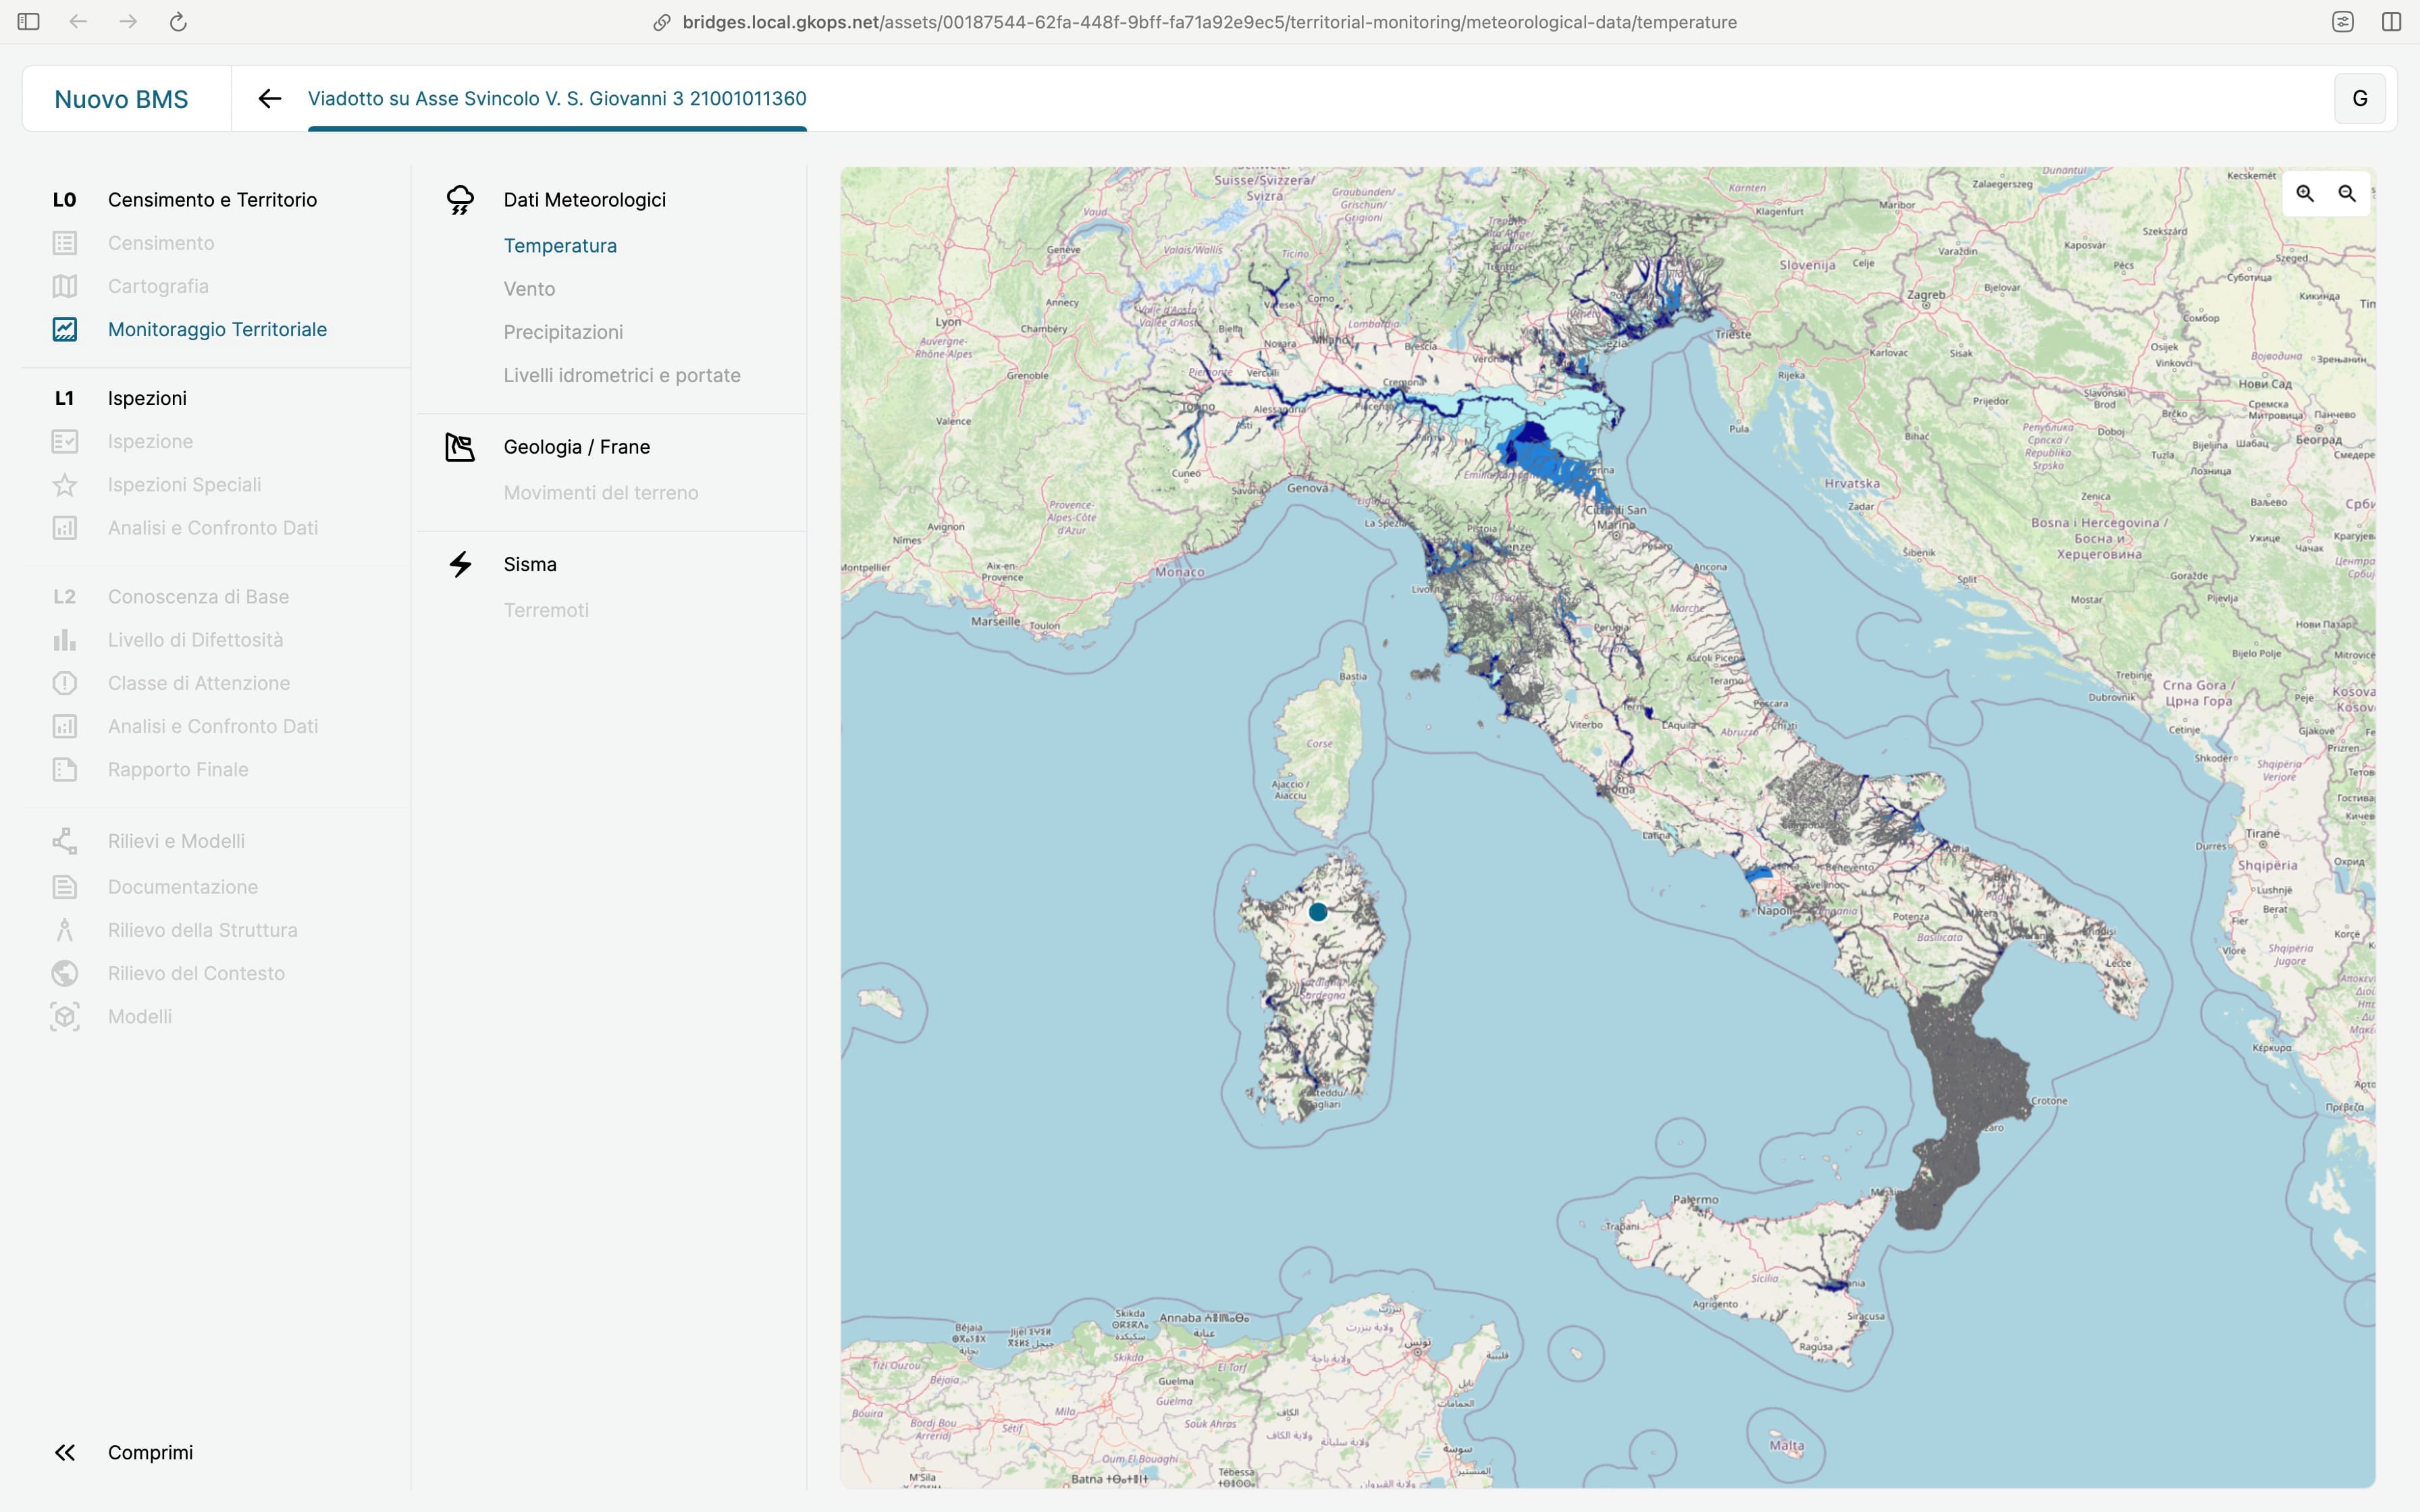
\includegraphics[width=1\textwidth]{Tesi/images/Capitolo5/italiaAlluvioni.jpg}
      \caption{Alluvioni - Estensione dell’area allagabile (PGRA 2021) - WMS}
      \label{fig:italiaAlluvioni}
\end{figure}

\subsection{Implementazione protocollo WMTS}

L'attenzione si è poi rivolta sulla possibilità di utilizzare il protocollo WMTS anziché WMS per servire la stessa mappa, poiché come già spiegato nel capitolo precedente, il primo protocollo offriva prestazioni migliori grazie all'uso delle tiles.
\\Quindi, il lavoro si è nuovamente spostato lato front-end, dovendo aggiungere all'interno del componente Angular il supporto al nuovo tipo di protocollo scelto. Per fare ciò, il tirocinante ha nuovamente modificato le classi \verb|BuildLayer.ts| e \verb|MapModel.ts|, realizzando un codice simile a quello precedentemente implementato per il protocollo WMS, utilizzando però le classi \verb|WMTSCapabilities| e \verb|WMTS|, anch'esse fornite dalla libreria di OpenLayers. Il processo iniziava con una richiesta al GeoServer tramite GetCapabilities, al fine di ottenere le informazioni sui layer disponibili e le relative proiezioni. Successivamente, una volta ricevuta la risposta, veniva eseguito un parser utilizzando la classe \verb|WMTSCapabilities| per estrapolare i layer interessati. Infine, si utilizzava la classe \verb|WMTS| per richiedere, tramite WMTS, le immagini a tiles direttamente al GeoServer. Queste immagini venivano quindi utilizzate per comporre e visualizzare la mappa nell'applicazione.
\\Lato back-end, nonostante tutti i servizi esterni fornissero solo le mappe tramite protocollo WMS, è stato sufficiente configurare il GeoServer affinché le pubblicasse tramite protocollo WMTS: come già spiegato, il GeoServer è in grado di gestire la conversione fra i due protocolli, andando internamente a trasformare le immagini della mappa in tiles, per poi esporle attraverso il nuovo protocollo.
\\Dopo aver constatato un netto miglioramento delle prestazioni, non solo è stato deciso di continuare ad utilizzare GeoServer come server di mappe, ma anche di ridurre drasticamente, dove possibile, l'impiego del protocollo WMS a vantaggio del WMTS.
\\L'immagine \ref{fig:italiaAlluvioniWMTS} mostra, attraverso gli strumenti per sviluppatori del browser, come il client effettuasse molteplici richieste, ottenendo così per ognuna di esse una tile, a differenza del vecchio protocollo che restituiva un'unica immagine.

\begin{figure}[htbp]
      \centering
      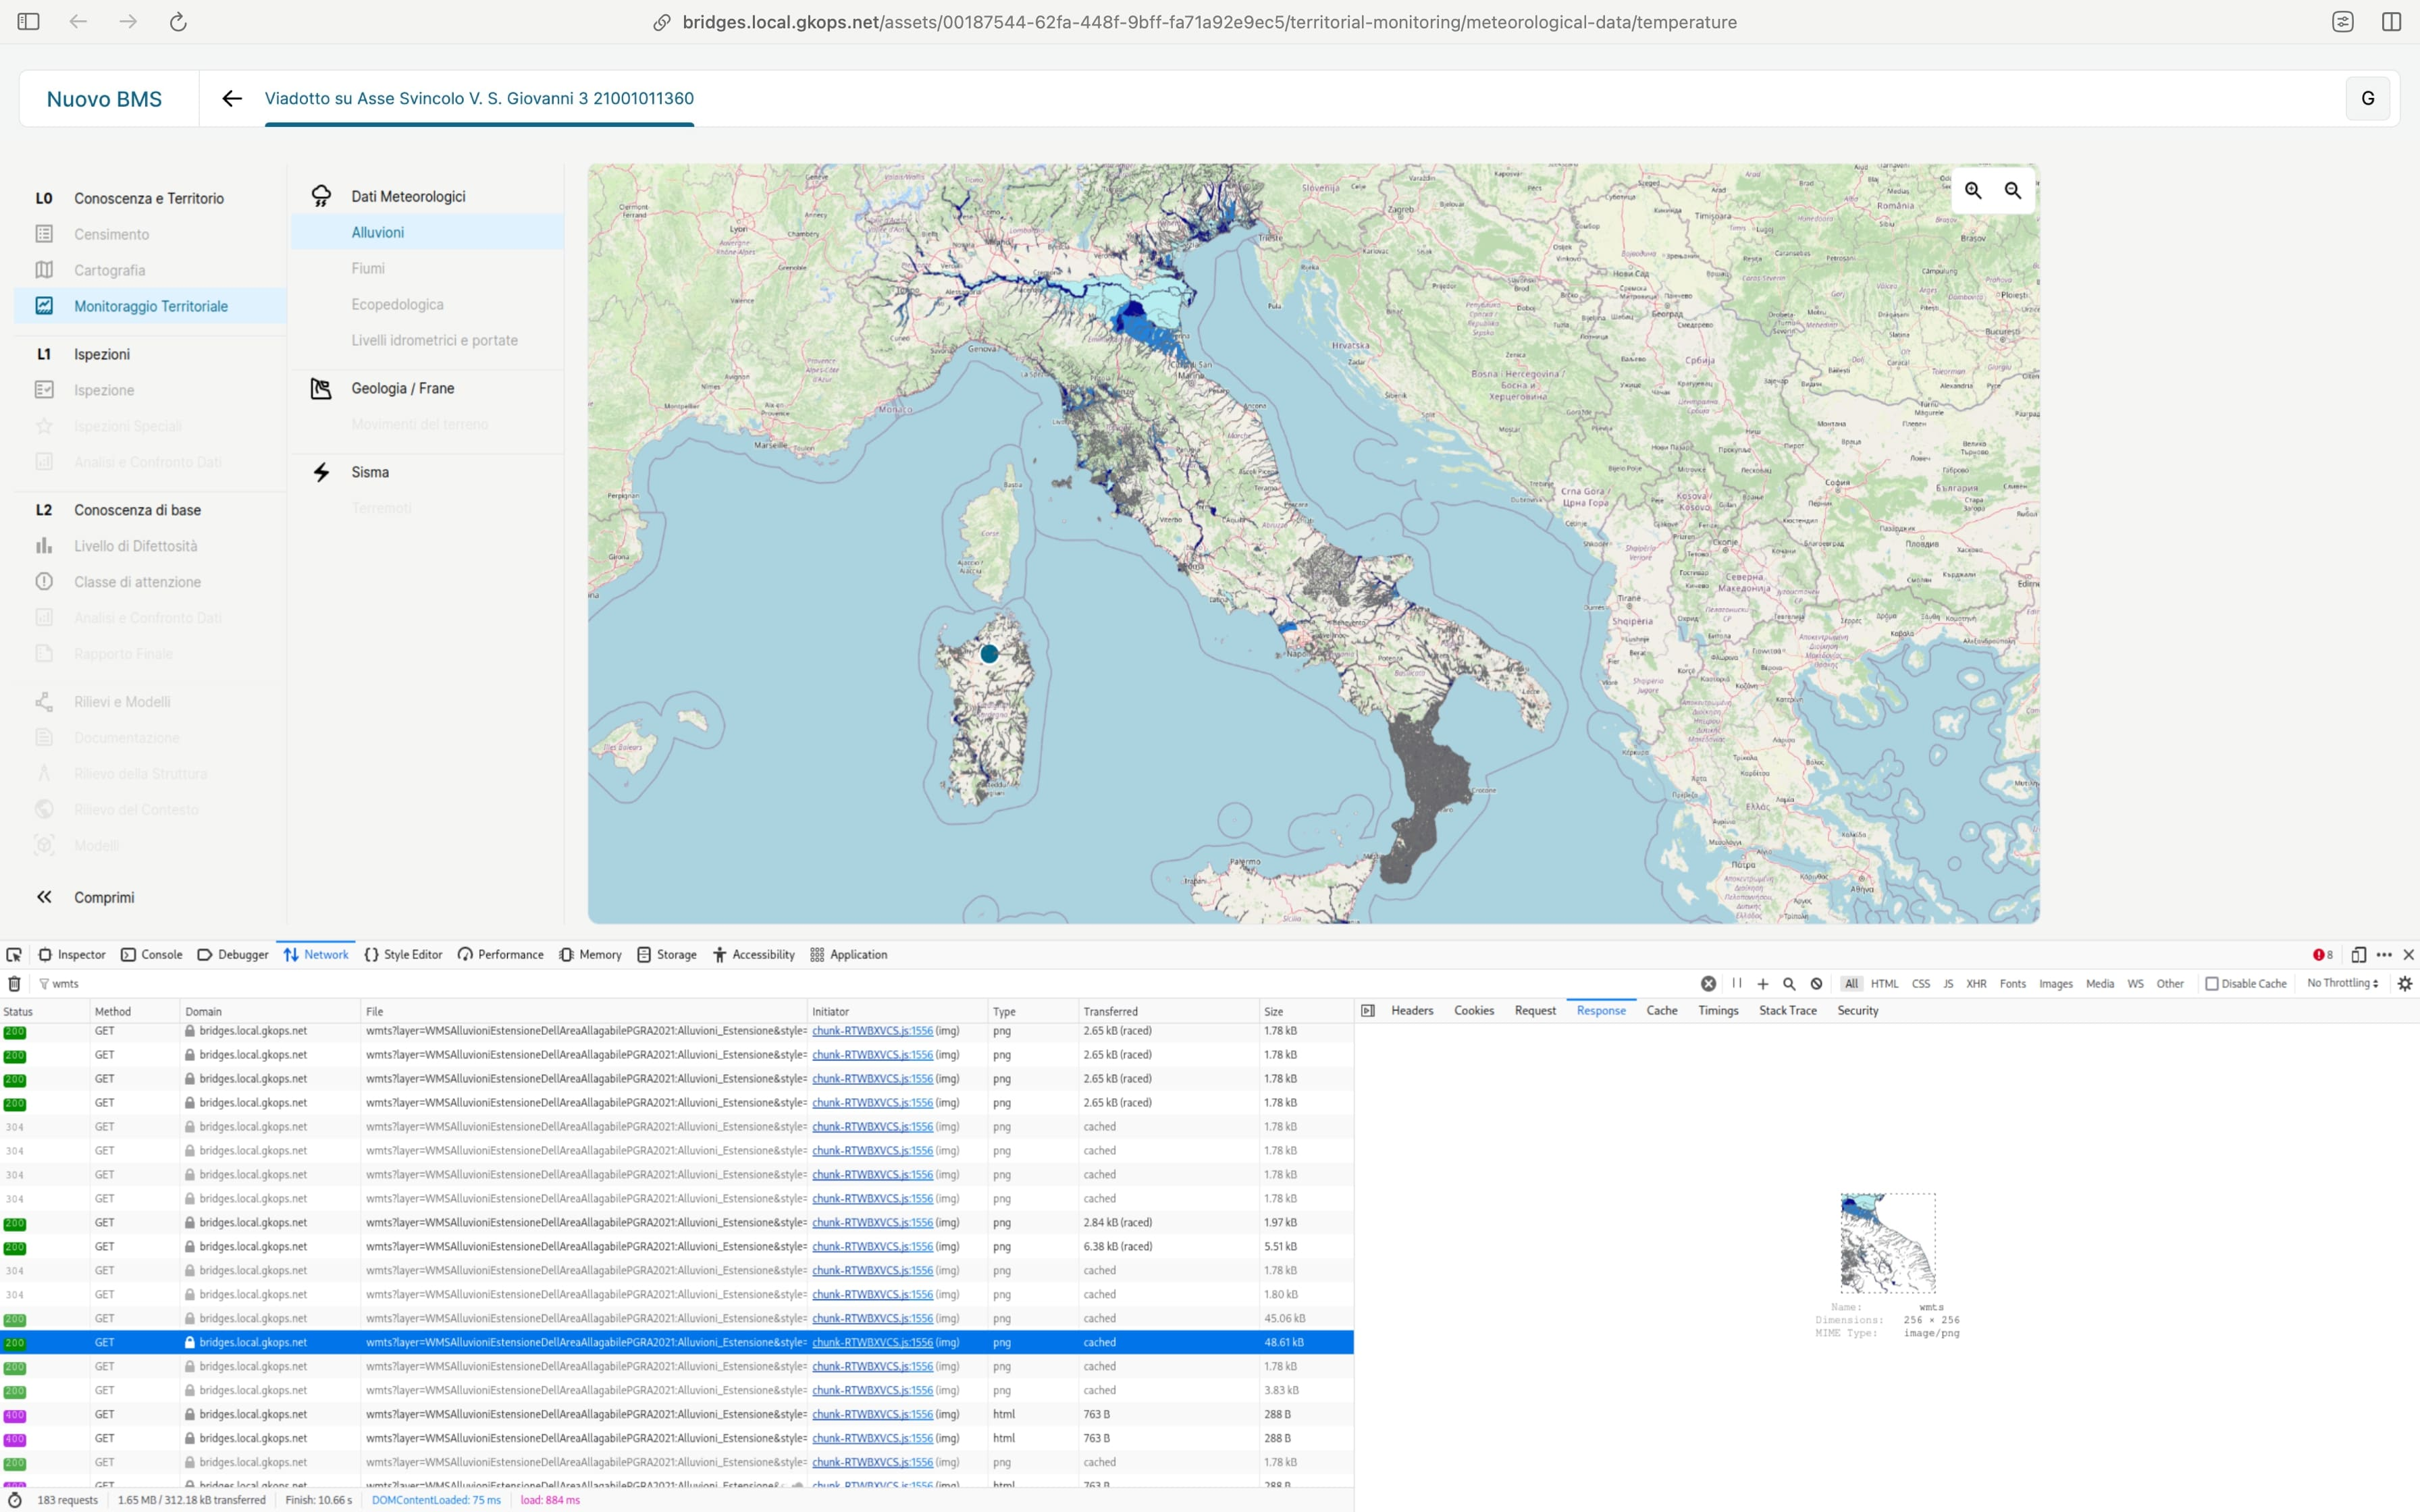
\includegraphics[width=1\textwidth]{Tesi/images/Capitolo5/italiaAlluvioniWMTS.jpg}
      \caption{Alluvioni - Estensione dell’area allagabile (PGRA 2021) - WMTS}
      \label{fig:italiaAlluvioniWMTS}
\end{figure}

\subsection{Implementazione del formato Shapefile}

Un altro formato di mappa geospaziale che doveva ancora essere implementato, era il formato shapefile, utilizzato dagli enti IdroGEO e GeoCart per fornire le loro mappe. Fino a quel momento, il formato shapefile non era stato considerato, in quanto OpenLayers non lo supporta nativamente. Di conseguenza, le mappe di GeoCart non erano ancora state integrate, mentre quelle di IdroGEO per semplicità erano state implementate soltanto in GeoJSON, dato che erano fornite anche in quel formato. 
\\Per risolvere il problema, si è inizialmente ipotizzato di passare attraverso l'uso di librerie di terze parti che consentissero la conversione del formato shapefile in un altro formato, come il GeoJSON. Tuttavia, con quel tipo di implementazione, sarebbero comunque persistite le problematiche già spiegate in precedenza, oltre al fatto che non ci sarebbe stata garanzia circa la correttezza della conversione al nuovo formato. Inoltre, considerata la mole degli shapefiles, sarebbe risultato necessario partizionare i dati e gestirne il recupero parziale.
\\Pertanto, si è pensato di appoggiarsi nuovamente al GeoServer, che supporta shapefile come formato e lo espone in vari protocolli, tra cui quelli fino ad ora implementati. Ciò ha ovviamente facilitato la parte di sviluppo, in quanto non è stato necessario programmare alcuna funzionalità per supportarlo: lato back-end, infatti, è stato sufficiente caricare il file della mappa all'interno del volume (del container Docker di GeoServer) e poi, utilizzando l'interfaccia grafica di GeoServer, renderlo disponibile come layer. Lato front-end, invece, non è stato necessario modificare alcuna classe, ed è bastato richiedere la nuova mappa al GeoServer come fatto precedentemente.
\\Per verificare il suo funzionamento è stata scelta una nuova mappa, fornita dall'ente GeoCart che rappresentava il "Reticolo Idrografico" nella regione della Calabria \ref{fig:calabriaAlluvioni}.
Per semplicità, il tirocinante ha deciso di far richiedere al client prima la mappa nel protocollo WMS, così da controllare se questa venisse rappresentata correttamente e nella giusta proiezione, e solo dopo averla verificata, farla richiedere anche in WMTS.
\\Infatti, l'unica problematica riscontrata in questa implementazione è stata che la mappa conteneva, all'interno del suo shapefile, una proiezione non nota a GeoServer, andando così a mostrare a schermo la mappa a delle coordinate sbagliate.
Per risolvere il problema, invece di utilizzare Proj4J come fatto precedentemente, è stato sufficiente, attraverso l'interfaccia grafica di GeoServer, impostare forzatamente una nuova proiezione: attivando l'impostazione "Force Declared", infatti, GeoServer si è occupato in automatico di sovrascrivere la vecchia proiezione con la nuova scelta, cercando di mantenere nel modo più fedele possibile la rappresentazione della mappa. Per limitare il rischio di errore dovuto al cambio di proiezione, è stato sufficiente cercare, con l'aiuto del tutor aziendale, una nuova proiezione che fosse compatibile con quella utilizzata all'interno dello shapefile, riuscendo così a mostrare correttamente la mappa a schermo. 
\\Inoltre, questa soluzione ha anche diminuito il carico di lavoro lato front-end, avendo spostato il compito di registrare ed eseguire il cambio di proiezione su GeoServer. Ovviamente, avendo caricato la mappa direttamente all'interno di GeoServer, senza dover passare da un server esterno come negli altri casi, la sua visualizzazione è stata pressoché immediata.
\begin{figure}[htbp]
      \centering
      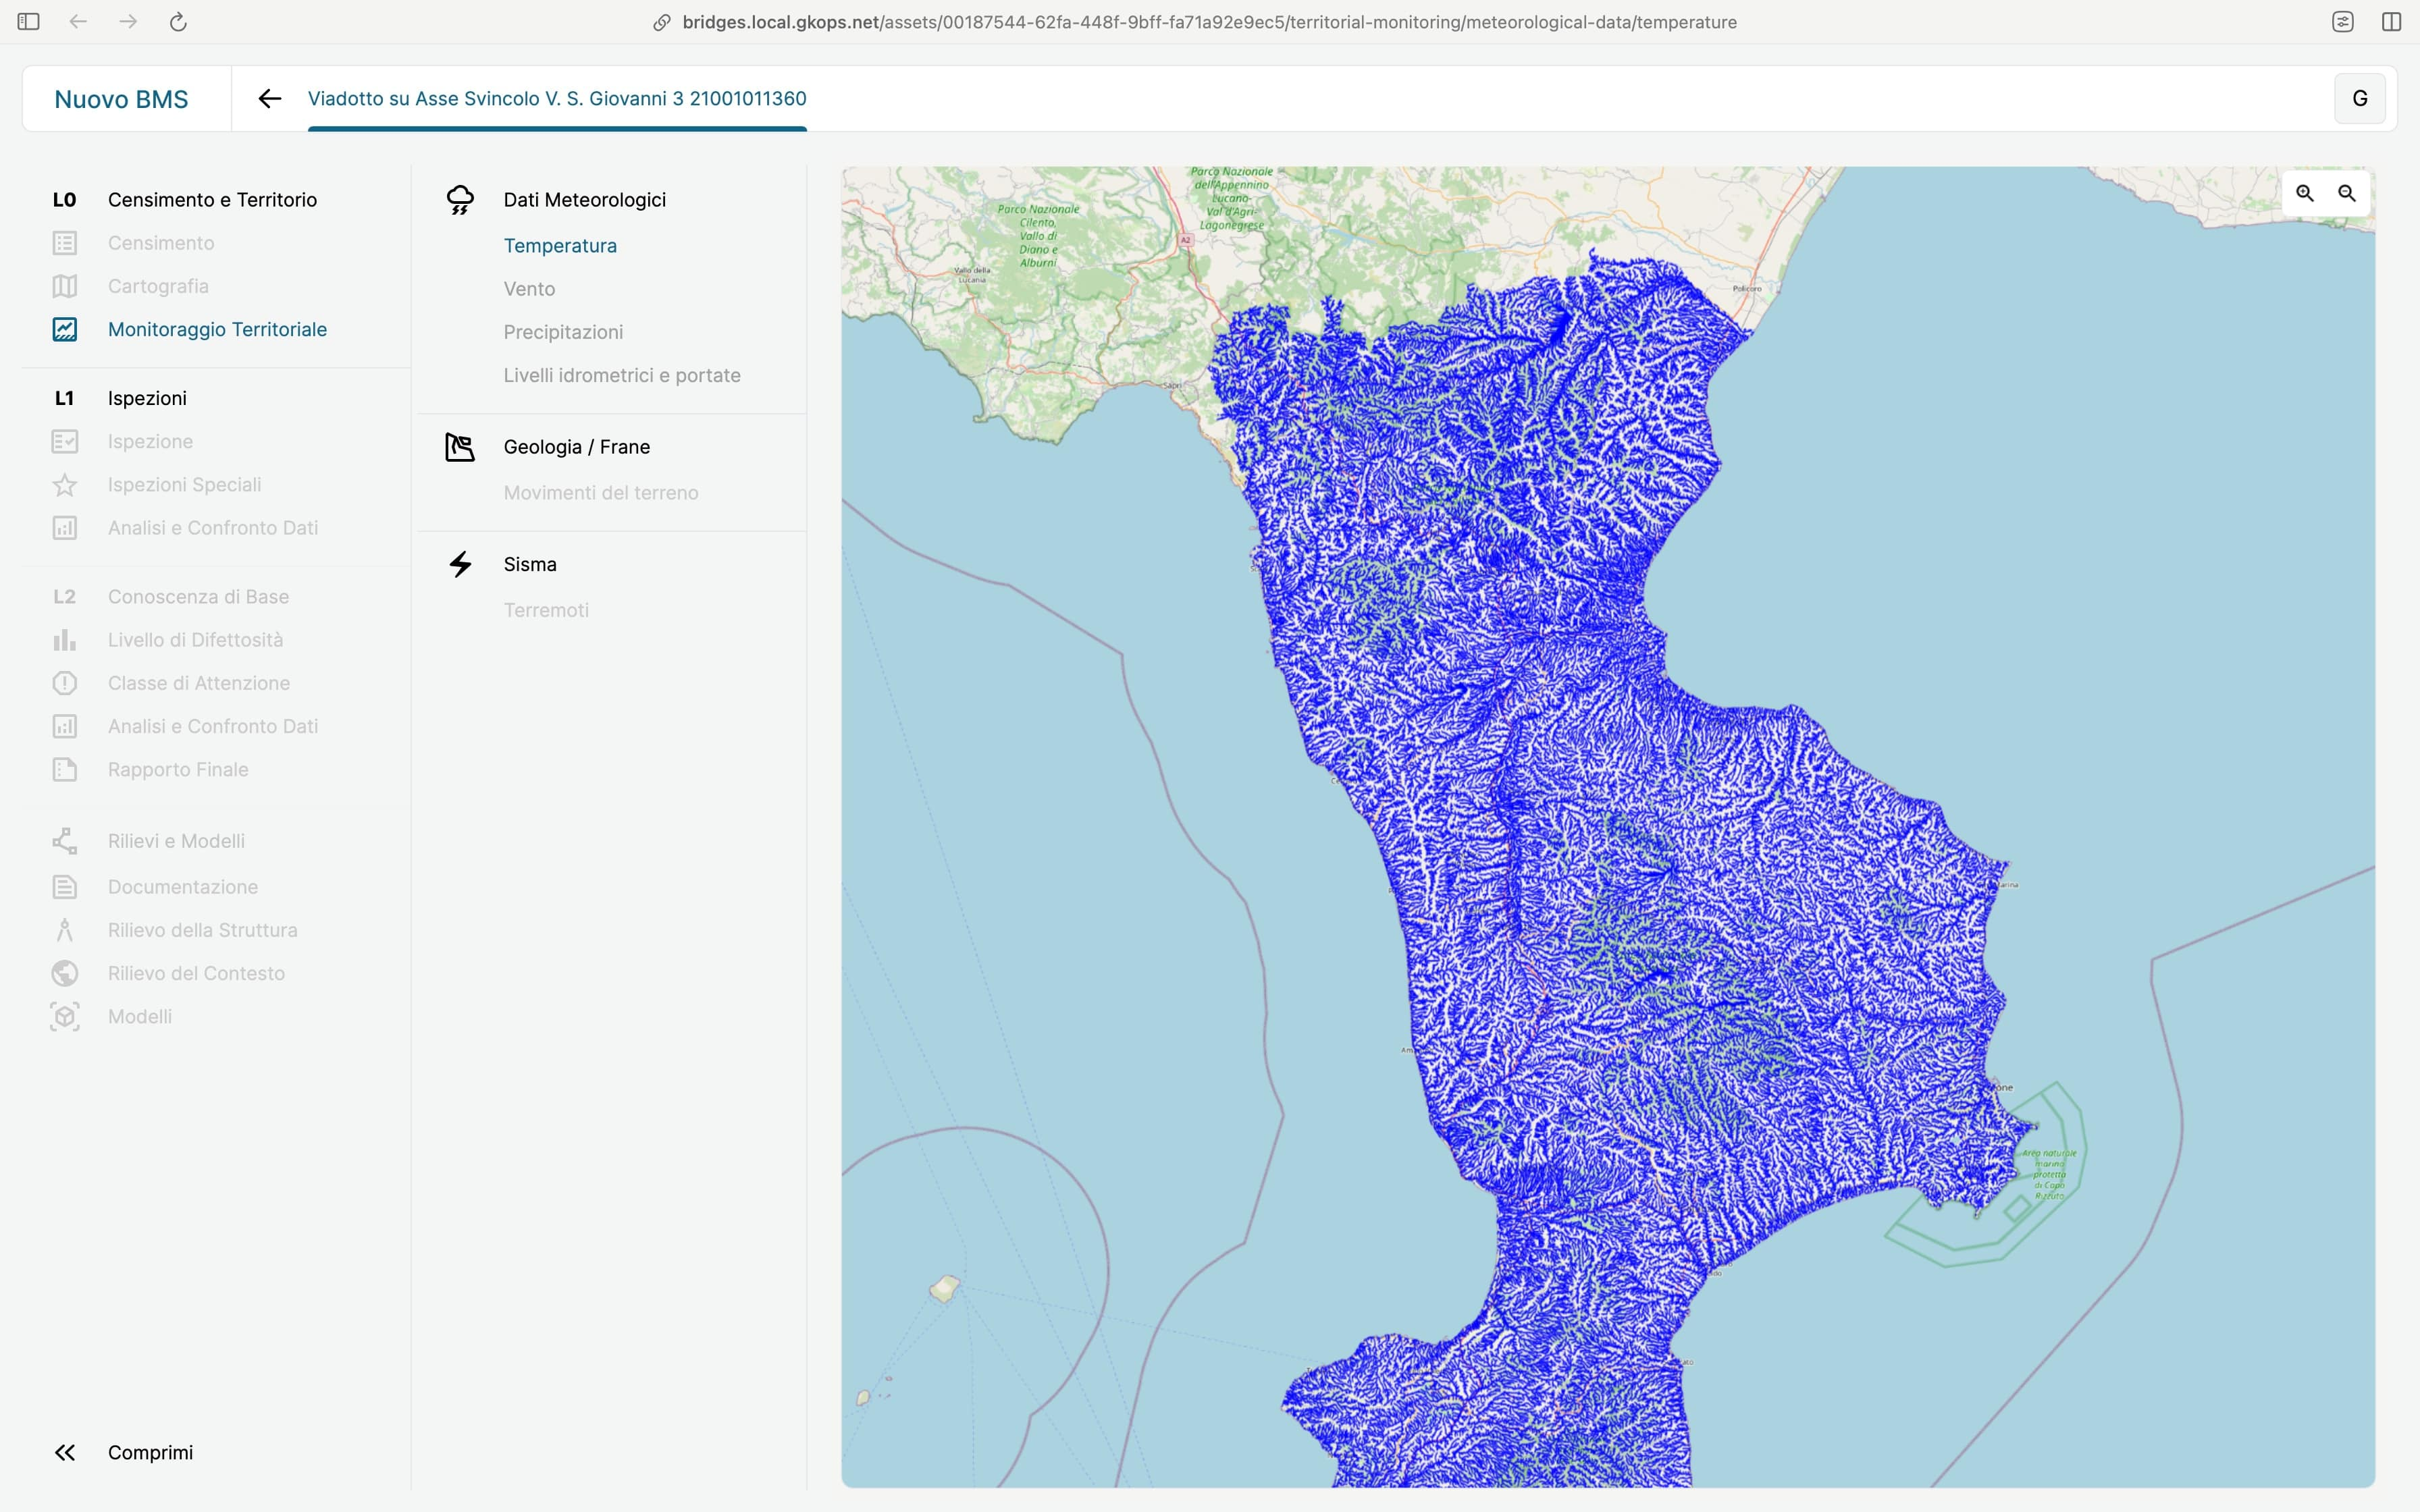
\includegraphics[width=1\textwidth]{Tesi/images/Capitolo5/calabriaAlluvioni.jpg}
      \caption{Calabria Reticolo Idrografico - WMTS}
      \label{fig:calabriaAlluvioni}
\end{figure}
\newpage
\subsection{Implementazione del formato SLD}

Alcune delle mappe fornite da questo ente, oltre al formato shapefile, comprendevano dei file aggiuntivi in formato SLD. Questi file si occupavano, similmente al ruolo del CSS nelle pagine HTML, di definire uno stile specifico per la rappresentazione dei dati della mappa. Questi file, inoltre, potevano contenere al loro interno l'immagine di una legenda, la quale serviva per rappresentare il motivo dello stile applicato alla mappa (generalmente, questo tipo di immagine è quello che viene restituito come risposta alla richiesta di GetLegendGraphic, nel protocollo WMS).
\\Il tirocinante si è quindi occupato di integrare all'interno del progetto le mappe con questo stile, sfruttando anche in questo caso le funzionalità offerte da GeoServer.
\\Il lavoro è cominciato inserendo al suo interno una delle mappe in formato shapefile, privandola del suo file di stile, in modo da osservare le differenze della mappa con e senza quest'ultimo applicato; oltre che verificare la posizione corretta della mappa. Questa, nota con il nome di "EGMS Calabria", è stata richiesta dal client sia tramite protocollo WMS che WMTS (utilizzando la stessa implementazione fatta precedentemente), riuscendo così in entrambi i casi a visualizzarla correttamente. Tuttavia, in maniera conforme alle previsioni, lo stile della mappa applicato non era quello corretto, e di conseguenza, la mappa veniva mostrata con lo stile di base fornito da GeoServer. Nell'immagine \ref{fig:calabriaNoSLD} viene mostrata la mappa con lo stile di default applicato da GeoServer.
\\~\\ %<- fixme
\begin{figure}[htbp]
      \centering
      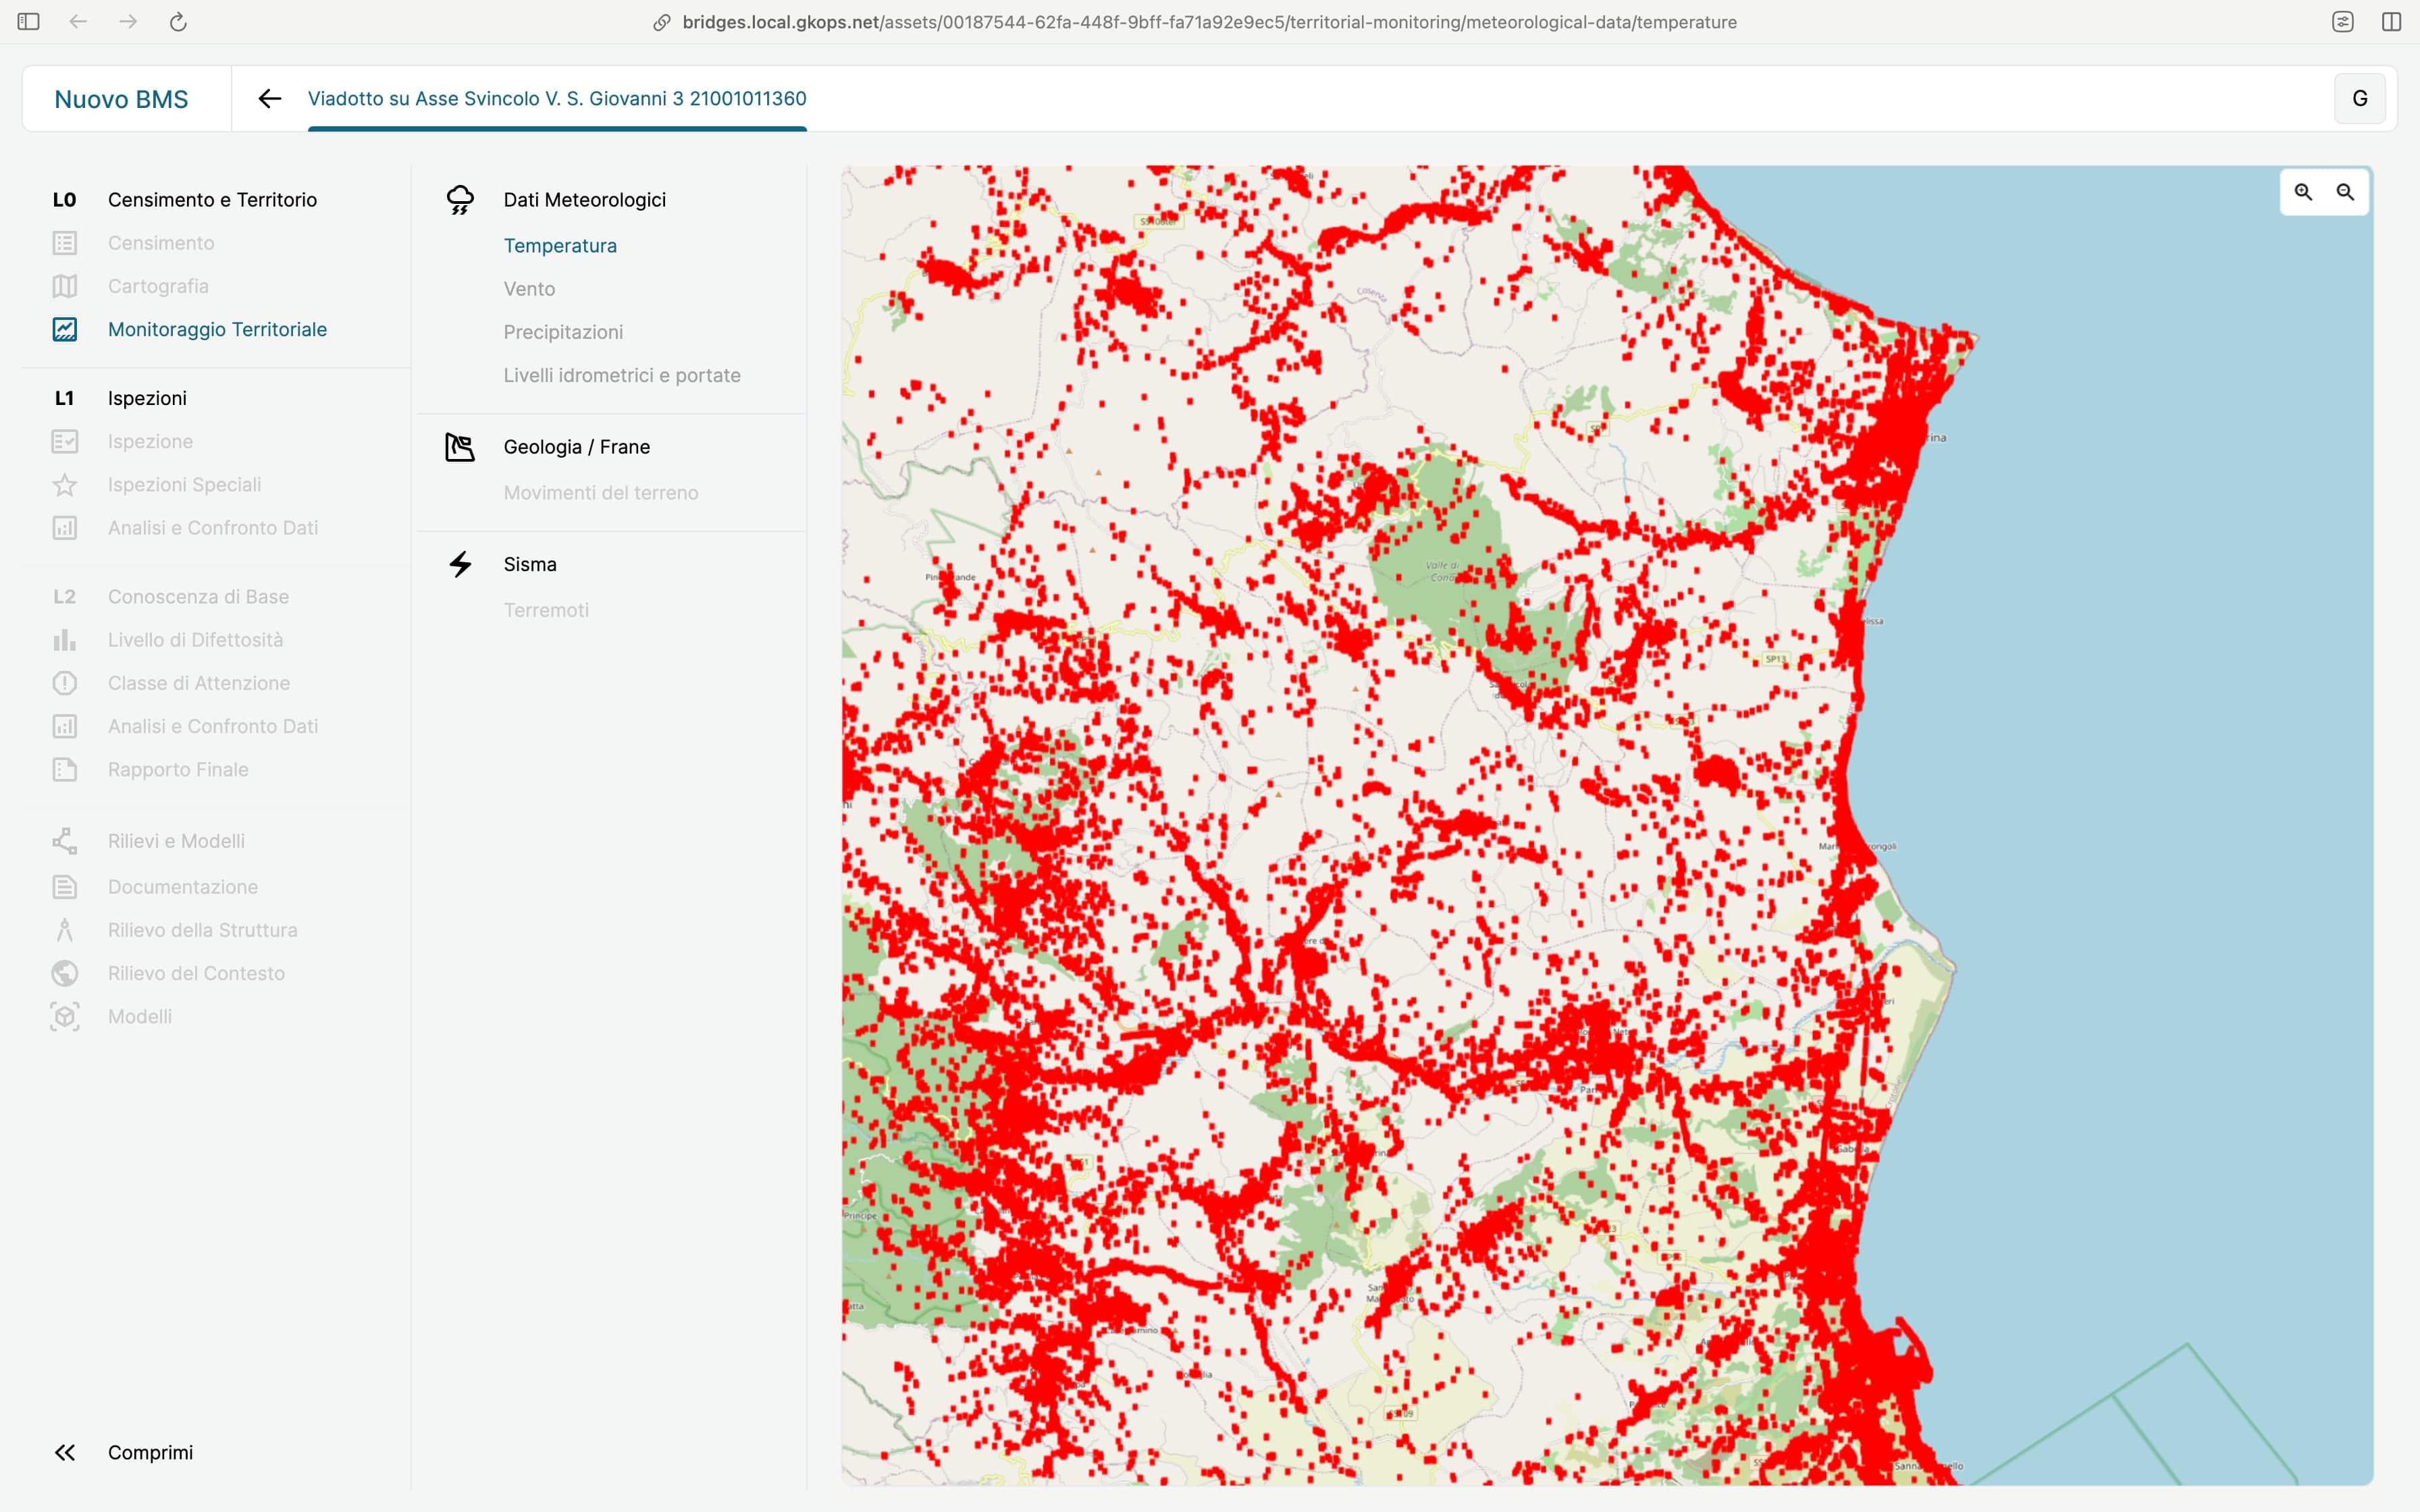
\includegraphics[width=1\textwidth]{Tesi/images/Capitolo5/calabriaNoSLD.jpg}
      \caption{EGMS Calabria - priva di stile SLD}
      \label{fig:calabriaNoSLD}
\end{figure}
\\Per applicare lo stile allo shapefile è stato prima caricato un nuovo file SLD (attraverso l'interfaccia grafica di GeoServer), seguendo una procedura simile a quella adottata per caricare una mappa e poi, è stato sufficiente selezionare la mappa su cui applicare lo stile. GeoServer offriva sia la possibilità di sovrascrivere lo stile corrente, applicando così quello appena caricato, sia di avere molteplici stili disponibili, in modo che il client potesse richiederne uno fra questi. Poiché erano presenti delle mappe che potevano essere visualizzate con più stili differenti, come ad esempio, la mappa scelta che aveva due file SLD chiamati "L2b Generale" e "L2b Dettagliato", si è scelto di non sovrascrivere lo stile ma di mantenerne molteplici.
\\Lato front-end, è stato quindi necessario modificare il codice affinché si riuscisse, oltre che a visualizzare la mappa, a richiedere al server quali fossero gli stili disponibili per quest'ultima. Queste informazioni, insieme a quelle riguardanti il layer (tipo di proiezioni, formato, etc...), erano ottenibili tramite la richiesta di GetCapabilities.
\\Quindi, il codice per recuperare la mappa mediante protocollo WMTS è stato ulteriormente modificato affinché, mediante \verb|WMTSCapabilities|, si riuscisse a estrapolare, oltre che al nome del layer e la rispettiva proiezione, anche l'elenco di tutti gli stili disponibili. Una volta ottenuto, è stato sufficiente passare come argomento alla classe \verb|WMTS| anche il nome dello stile da visualizzare.
\medskip
\\L'ultimo compito da svolgere è stato quello di riuscire a far ottenere l'immagine della legenda al front-end, in modo da poterla visualizzare affiancata alla mappa stessa. La legenda, salvata anch'essa all'interno di GeoServer, poteva essere reperita attraverso una richiesta di GetLegendGraphic, mediante protocollo WMS. Poiché il client era già a conoscenza delle informazioni della mappa, in quanto aveva appena compiuto una richiesta di GetCapabilities tramite protocollo WMTS, non gli era necessario, per ottenere la legenda, fare di nuovo una richiesta di GetCapabilities tramite protocollo WMS, ma gli era sufficiente richiedere direttamente l'immagine della legenda con la richiesta GetLegendGraphic.
\\Il codice è stato quindi nuovamente modificato, facendo in modo che, a seguito della visualizzazione della mappa, il front-end effettuasse una nuova richiesta HTTP al GeoServer, così da recuperare direttamente l'immagine della mappa. Nell'immagine \ref{fig:calabriaSLDLegenda} è mostrata la mappa con lo stile SLD applicato, accompagnata dalla relativa legenda.
\begin{figure}[htbp]
      \centering
      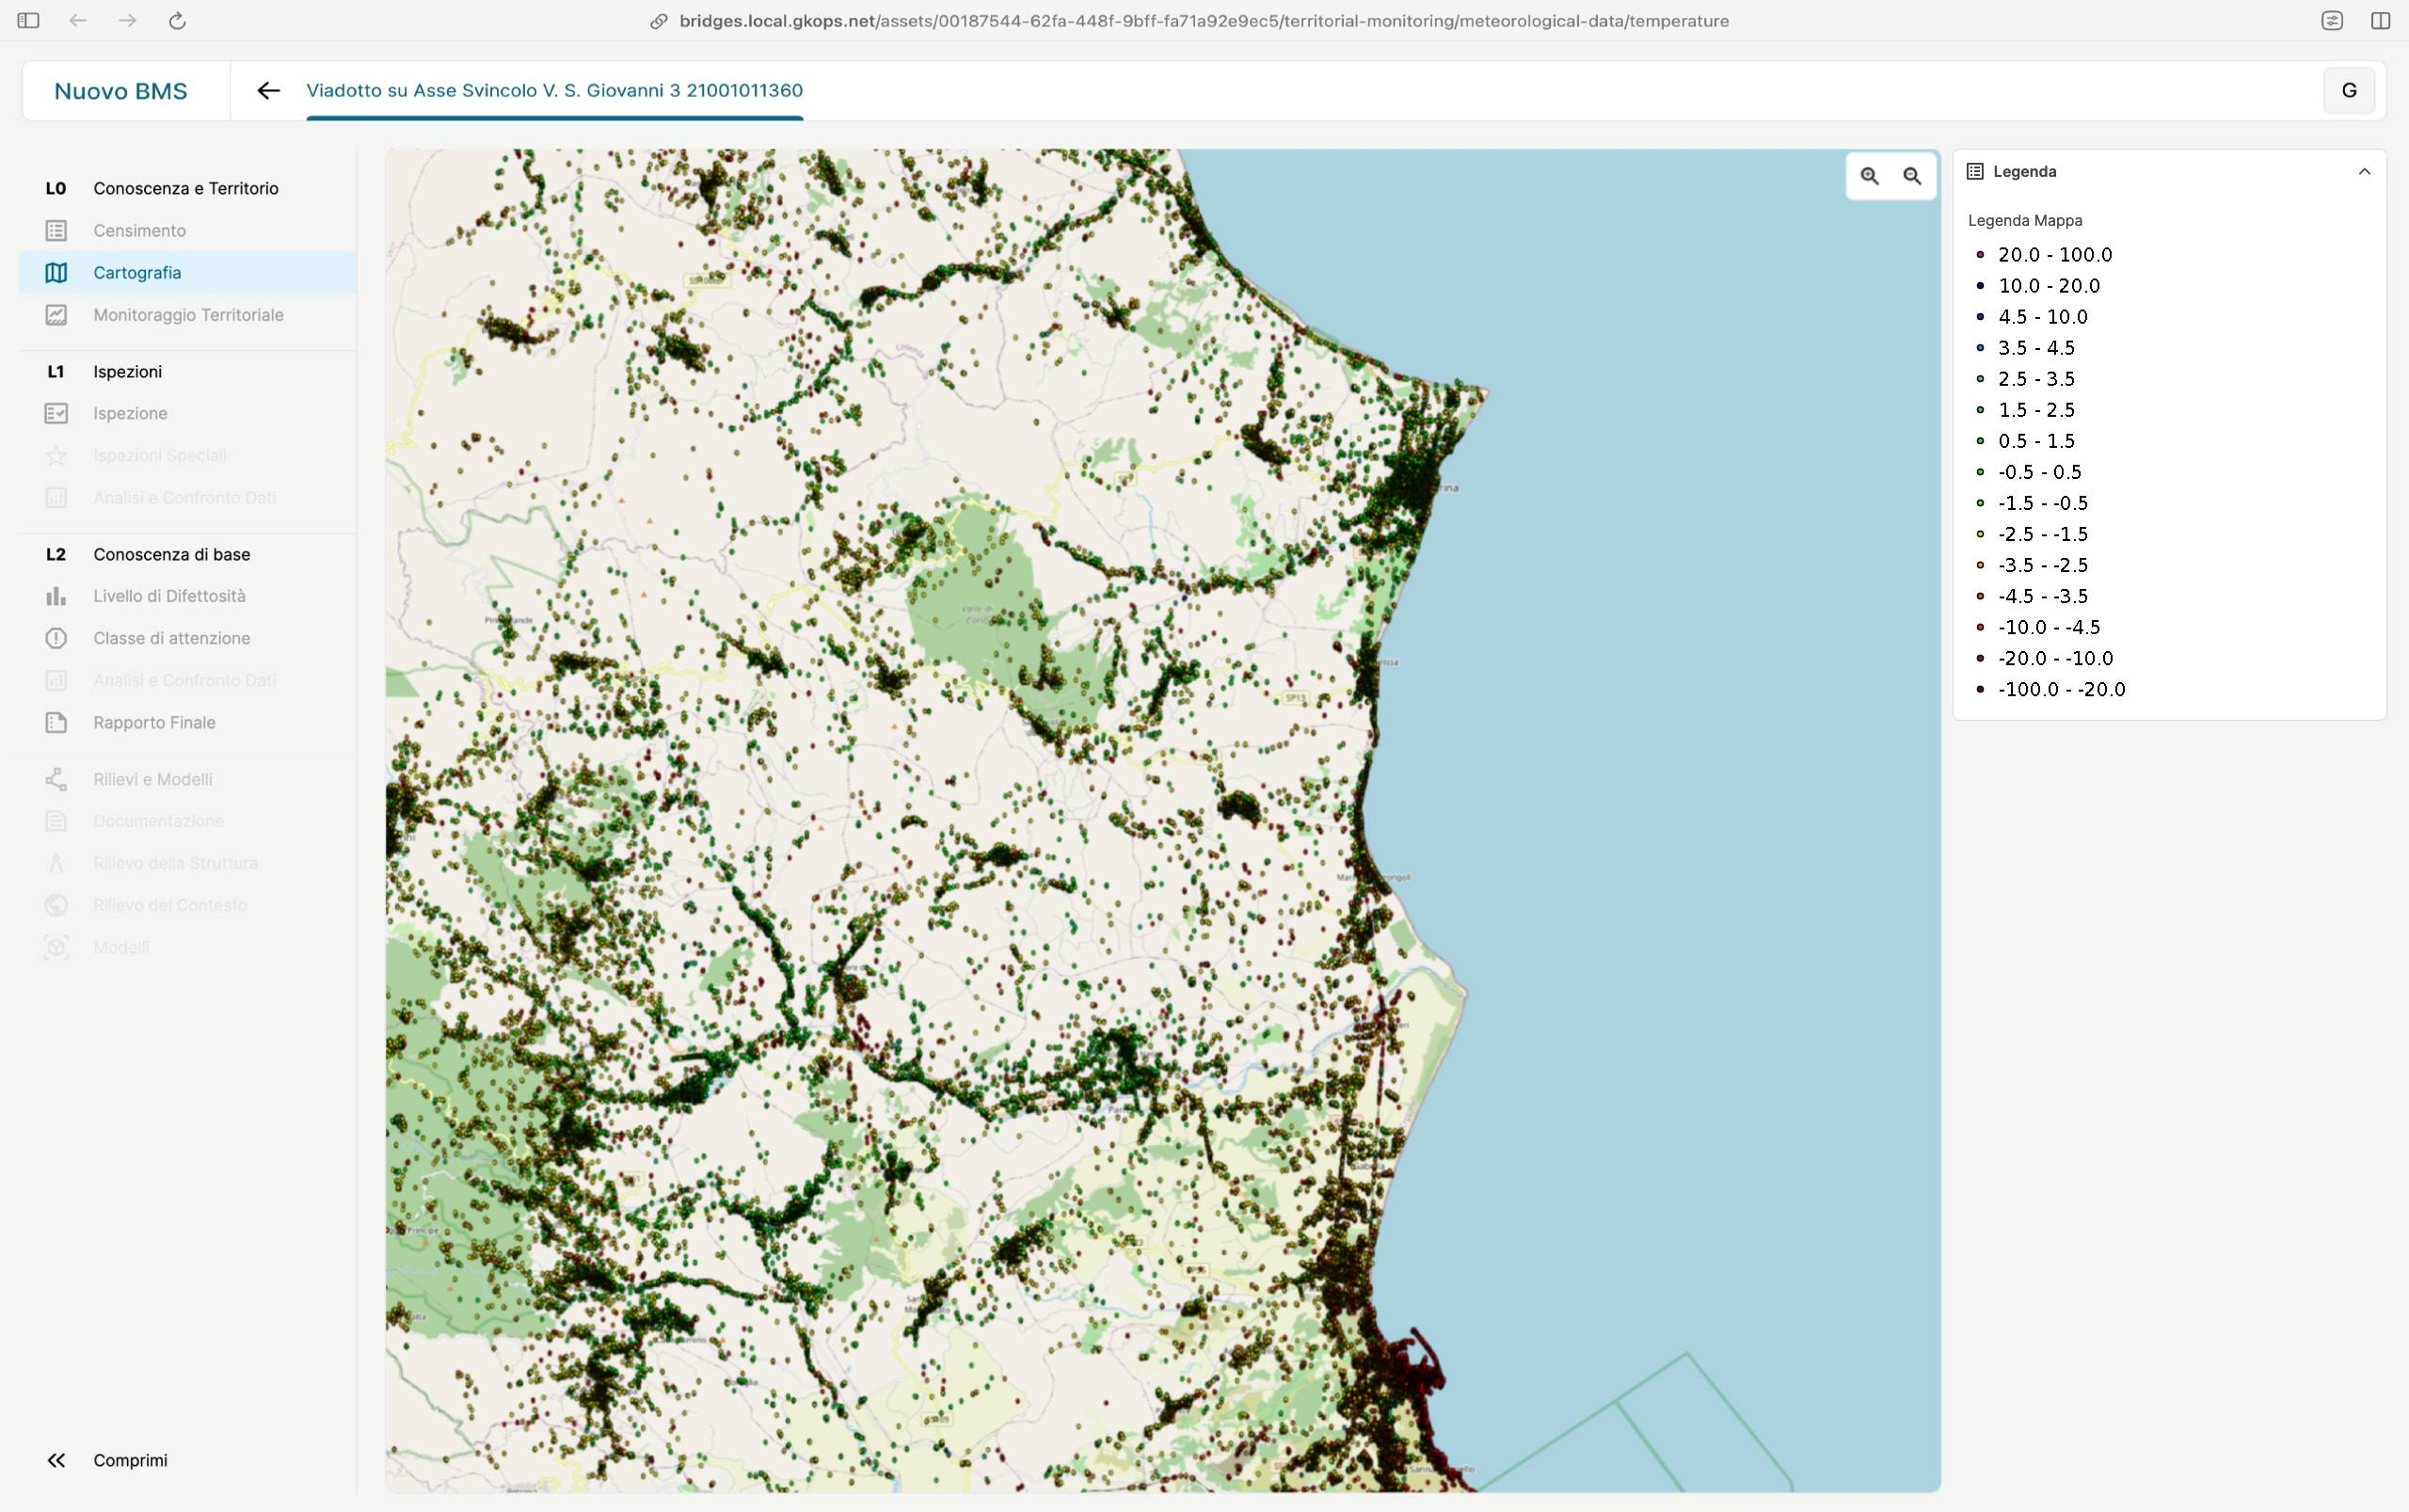
\includegraphics[width=1\textwidth]{Tesi/images/Capitolo5/calabriaSLDLegenda.jpg}
      \caption{EGMS Calabria - con stile SLD applicato}
      \label{fig:calabriaSLDLegenda}
\end{figure}

\subsection{Implementazione protocollo WFS}

L'ultima implementazione rimasta da fare era quella del protocollo WFS. Per renderlo supportato dal front-end, è stato sufficiente sviluppare un codice simile a quello utilizzato precedentemente per il formato GeoJSON, con l'unica differenza di contattare direttamente il GeoServer, invece di recuperare i dati della mappa dal file locale salvato nel progetto. Il GeoServer, infatti, offriva la possibilità di fornire i dati delle mappe anche in questo formato (per il protocollo WFS), evitando così di dover scrivere ulteriore codice per supportarne uno nuovo.
\\In maniera analoga alle altre implementazioni, il candidato ha innanzitutto modificato le classi \verb|BuildLayer| e \verb|MapModel|, aggiungendo come nuovo tipo il WFS. Successivamente, come fatto per il GeoJSON, ha di nuovo utilizzato la stessa classe (chiamata anch'essa \verb|GeoJSON|) fornita dalla libreria OpenLayers stessa. A quest'ultima ha infine passato come argomento l'url della mappa da reperire, invece del percorso locale all'interno del progetto. Precisamente, l'url corrispondeva ad una richiesta di GetFeature al GeoServer, richiedendo tramite query parameters: il formato della mappa (richiesto appunto in JSON), il nome della mappa, la proiezione e infine un parametro che permetteva di limitare il numero di feature da farsi restituire dal server. Infatti, a differenza della vecchia implementazione, il GeoServer (mediante protocollo WFS) permetteva di effettuare delle manipolazioni sulle feature, prima che queste venissero effettivamente restituite. Da quel momento, è stato quindi possibile far richiedere dal client, se necessario, una serie di parametri aggiuntivi all'interno della richiesta che permettessero operazioni come l'ordinamento, il filtraggio, etc...
\\Tali operazioni potevano essere svolte anche unicamente lato front-end, ma come già spiegato, ciò avrebbe richiesto un dispendio elevato di risorse, in quanto tutte le feature sarebbero dovute essere tenute in memoria.
\chapter{Sviluppo Back-end per l'inserimento di mappe}
\label{cap:chapter6}

\section{Programma AutoLoader}
 
Dal momento che tutti i formati di mappe erano stati testati ed integrati, riuscendo quindi ad avere per ognuna di loro un'implementazione funzionante lato front-end, ciò che rimaneva da fare, oltre che a migliorare l'integrazione tra front-end e back-end, era la realizzazione di un meccanismo che consentisse il caricamento automatico di tutte le mappe all'intero di GeoServer. Fino ad allora, infatti, soltanto alcune delle mappe erano state caricate, e quelle poche servivano ad avere un'implementazione funzionante per quei formati. Infatti, il front-end, anche se in maniera "hard coded", riusciva a richiedere le mappe nei protocolli WMTS (quando possibile), WMS e WFS al GeoServer, oltre che a supportare gli stili personalizzati nel formato SLD. 
\\In questa seconda fase di sviluppo, quindi, lo scopo del tirocinante è stato quello di realizzare un sistema, che prende il nome di AutoLoader, per il caricamento automatico di tutte le mappe all'interno di GeoServer.  Questo permetteva non solo di verificare che tutte le mappe funzionassero correttamente con le implementazioni da lui effettuate, ma anche di prepararle per l'integrazione all'interno del sistema stesso.

\subsection{Risoluzione del problema della Rest API}

L'idea principale dietro questo programma era quella di sviluppare un'applicazione in C\# che, sfruttando la REST API fornita da GeoServer, fosse in grado di creare automaticamente delle Workspace e degli Storage in cui caricare le mappe, per poi pubblicare tutti i layer presenti al loro interno. Per selezionare quali mappe caricare all'interno di GeoServer, si è deciso di far leggere al programma i dati da un file CSV, utilizzando come base di partenza quello realizzato dal candidato i primi giorni di tirocinio.
\\Il problema principale con questa implementazione è che le API fornite da GeoServer, come viene riportato dagli sviluppatori nella loro documentazione \cite{DocumentazioneGeoServerAPI}, presentano tutt'ora alcune criticità importanti che possono influenzare il suo utilizzo e la sua affidabilità. Innanzitutto, la specifica della REST API è rimasta alla versione di Swagger 2.0 e non è aggiornata al nuovo standard di OpenAPI 3.0. Ciò ha chiaramente comportato una peggiore comprensione e utilizzo dell'API stessa, ma sopratutto, viene fatto notare che i file di Swagger utilizzati per documentare l'API sono stati creati manualmente nel 2017 e non sono stati più aggiornati con l'evoluzione dell'infrastruttura del software: 
\begin{quote}
``Warning The API is documented as Swagger 2.0 files. However, these files have been written by hand back in 2017, and have not always been kept up to date with the evolution of the GeoServer configuration object structure. Also, they have not been tested for proper client generation, and will likely not work for that purpose. Take them only as a form of documentation.''
\end{quote}
\\L'utilizzo dell'API di GeoServer, purtroppo, è stata una parte cruciale durante questa fase di sviluppo, e questo problema ha rappresentato una sfida significativa, in quanto è stato necessario sistemare manualmente le richieste, al fine di poterle poi utilizzare correttamente.
\\~\\
Il tirocinante si è dunque dedicato allo studio del linguaggio di programmazione C\#, e alle API messe a disposizione dal server di mappe. Il lavoro è poi proseguito sviluppando un programma, inizialmente esterno al progetto, capace di contattare il servizio di GeoServer; quest'ultimo avviato localmente attraverso un container Docker.
\\Per comunicare con la sua REST API, anziché scrivere un programma da zero per gestire manualmente ogni richiesta HTTP, dovendo quindi realizzare per ciascuna di esse una struttura dati apposita (con cui gestire e manipolare le richieste), è stato deciso di utilizzare una libreria opportuna. Tale libreria, nota con il nome di NSwag, permette di contattare il servizio REST API in automatico, senza doversi preoccupare di fare tutto quello descritto precedentemente. Nel dettaglio, questa libreria richiede come input il file YAML che descrive la specifica della REST API, attraverso la quale NSwag genera una o più classi contenenti a loro interno dei metodi già implementati, permettendo così di contattare il servizio.
\\La struttura dell'API di GeoServer, come molte altre, era organizzata ad endpoint, ognuno dei quali forniva delle funzionalità diverse. In questo modo era quindi possibile per il tirocinante contattare solamente quelli che possedevano le funzionalità a lui interessate. Inoltre, ogni endpoint possedeva il file Yaml della loro specifica REST API, fondamentale a Nswag per generare i metodi e le classi sopra citate.
\\Il candidato ha quindi scelto i seguenti endpoint, essenziali per la realizzazione del programma AutoLoader: 
\begin{itemize}
    \item \verb|/workspace|: questo endpoint contiene le richieste HTTP necessarie per creare, modificare, o eliminare le workspace all'interno di GeoServer;
    \item \verb|/wmsstores|: in maniera analoga a quello precedente, questo contiene tutte le richieste HTTP utili per creare, modificare, o eliminare uno storage WMS all'interno di una Workspace;
    \item \verb|/wmslayers|: questo endpoint, invece, contiene le operazioni relative ai layer all'interno di uno storage WMS. Oltre alle operazioni di base (come negli endpoint precedenti), permette di richiedere l'elenco di tutti i layer pubblicati e non, oltre a consentire la loro pubblicazione;
    \item \verb|/datastores|: consente di eseguire operazioni su tutti gli altri storage diversi dallo storage WMS o WMTS. Ad esempio, viene utilizzato per operare su uno storage WFS, o per lavorare su uno storage che contiene uno Shapefile;
    \item \verb|/featuretypes|: questo endpoint, infine, offre tutte le operazioni per lavorare con le feature presenti all'interno di un data store. In maniera analoga a \verb|/wmslayers|, permette di richiedere l'elenco di tutte le feature pubblicate e non, oltre a consentirne la pubblicazione;
\end{itemize}
\\Dopo aver generato con successo le classi tramite NSwag, il tirocinante ha quindi iniziato a verificare se i metodi al loro interno funzionassero correttamente, procedendo, per ognuno di essi, ad invocarli all'interno del programma. Poiché la specifica riportata non rispettava minimamente ciò che il GeoServer richiedeva, i metodi così generati risultavano non funzionanti, costringendo così il tirocinante a doverli riparare. Per fare ciò, è ricorso all'uso del comando cURL e del software Postman, affinché potesse controllare, con l'avanzare dello sviluppo dell'applicazione, che tutte le richieste corrispondessero a quanto descritto nella documentazione di SwaggerUI. Nel caso in cui ci fossero state delle discrepanze tra le richieste e quanto documentato, quindi, il tirocinante sarebbe dovuto intervenire modificando manualmente il file YAML fornito. 
%un esempio di yaml malformato?
\\Successivamente, il candidato ha deciso creare una nuova classe in cui, seguendo il Wrapper Design Pattern, ha incapsulato tutti i metodi autogenerati da NSwag, riuscendo così ad avere una organizzazione più pulita del codice e degli argomenti passati alle funzioni. All'interno di questa classe (che è diventata quella principale del programma), il tirocinante ha poi aggiunto dei nuovi metodi che consentivano di eseguire delle operazioni automatiche che normalmente non erano fornite dalla REST API stessa. Tra questi, il più importante è stato il metodo \verb|AddNewMapAsync()|, il quale consentiva di caricare automaticamente una mappa all'interno di GeoServer.

\subsection{Risoluzione del problema di identificazione dei Layer}

Normalmente, quando si vogliono caricare delle mappe al suo interno, si passa o un servizio di mappe esterno (come un server WMS), oppure si carica direttamente un file geospaziale (come ad esempio uno Shapefile): in entrambi casi, può succedere che al loro interno ci possano essere più layer da pubblicare. 
\\Il GeoServer, per diversificare quest'ultimi, utilizza come identificativo esattamente il nome del layer associato al nome della workspace in cui si trova (invece che utilizzare, banalmente, un numero come id oppure una funzione di hashing). Ad esempio, se viene caricata una mappa all'interno di GeoServer, quest'ultima verrà identificata nel seguente modo: \verb|nome_workspace:nome_layer|.
\\Durante il caricamento delle mappe è capitato che diverse fonti avessero al loro interno dei layer con lo stesso nome, portando quindi ad un errore nel loro inserimento, poiché non potevano esistere più layer con lo stesso nome associati alla medesima workspace.
\\Per evitare questo problema, il tirocinante ha proposto di creare una workspace separata per ogni servizio di mappe, invece di inserire tutti i servizi nella stessa workspace con i loro rispettivi layer. Di seguito è mostrata un'immagine che descrive meglio come è stata organizzata la gestione delle mappe all'interno di GeoServer.
\\~\\
\begin{minipage}{0.5\textwidth}
\dirtree{%
.1 Single Workspace.
.2 WMS Storage.
.3 layer 1.
.3 layer 2.
.3 layer **.
.2 WMS Storage 2.
.3 layer 1.
.3 layer 2.
.3 layer **.
.2 ShapeFile Storage.
.3 layer 1.
.3 layer 2.
.3 layer **.
}
\textbf{Old File Structure}
\end{minipage}%
\begin{minipage}{0.5\textwidth}
\dirtree{%
.1 Workspace WMS Storage 1.
.2 WMS Storage 1.
.3 layer 1.
.3 layer 2.
.3 layer **.
.1 Workspace WMS Storage 2.
.2 WMS Storage 2.
.3 layer 1.
.3 layer **.
.1 Workspace ShapeFile Storage 1.
.2 ShapeFile Storage 1.
.3 layer 1.
.3 layer **.
}%
\textbf{New File Structure}
\end{minipage}
\\~\\\smallskip
\\Il metodo \verb|AddNewMapAsync()| è stato quindi modificato per far sì che potesse inserire le mappe seguendo la nuova struttura appena descritta. 

\subsection{Struttura del file CSV}

Come già accennato, il file da fornire come input all'AutoLoader è stato creato partendo dal CSV di base fatto durante i primi giorni di tirocinio. Utilizzando quest'ultimo come riferimento, è stato possibile recuperare tutti i nomi delle mappe e le relative URI necessarie per accedere ai dati. Tuttavia, il file originale conteneva solo un elenco parziale delle mappe, in quanto erano presenti solo quelle fornite dai server esterni e non gli shapefile, poiché fino ad allora non era stato necessario includerli.
\\Di conseguenza, oltre a fare in modo che il programma leggesse il contenuto del CSV, c'era bisogno di realizzare un altro programma, più piccolo, che riuscisse ad estendere la tabella, aggiungendo in automatico delle nuove righe per rappresentare anche gli shapefile. Per fare ciò, il candidato si è servito di un'altra libreria, nota con il nome di CsvHelper, utile a manipolare ed analizzare i file CSV in modo più efficiente. Il tirocinante ha così realizzato un ulteriore programma, che ricorsivamente, andava ad esplorare tutti gli shapefile presenti all'interno delle cartelle di GeoServer: per ogni file trovato, attraverso l'uso di CsvHelper, veniva aggiunta una nuova riga all'interno della tabella, inserendo in una colonna apposita il percorso del file appena trovato. 
\\Il file CSV è stato così modificato, ottenendo infine una struttura comprendente:
\begin{itemize}
    \item \verb|Workspace Name|: questo campo serviva ad identificare il nome che poi il programma avrebbe utilizzato per creare la nuova Workspace all'interno di GeoServer;
    \item \verb|Service Name|: conteneva il nome dello storage che il programma avrebbe fatto creare a GeoServer;
    \item \verb|URI|: questa colonna conteneva o il link alle GetCapabilities da contattare, nel caso in cui si inserisse una mappa proveniente da un server esterno, oppure il percorso dello shapefile da caricare all'interno di GeoServer;
    \item \verb|Type|: indicava il tipo di fonte di mappa che si stava aggiungendo, se WMS, WFS o uno Shapefile. In base a ciò, il programma AutoLoader cambiava le sue richieste HTTP da inviare a GeoServer. Ad esempio, se inviare la richiesta HTTP per creare un DataStorage o uno storage WMS, oppure pubblicare un layer rispetto ad una feature;
    \item \verb|Status|: indicava eventuali problemi relativi alla mappa. Se il campo era vuoto, il programma caricava la mappa all'interno di GeoServer. Se invece veniva inserito un valore, di solito una descrizione del problema, il programma saltava la riga e procedeva con la successiva;
\end{itemize}
Qui di seguito viene riportato un esempio di tabella che illustra graficamente la struttura appena descritta.
\begin{table}[htbp]
    \caption{Esempio di file CSV per l'AutoLoader}\label{tab:labelTabella}
    \centering
    \resizebox{\textwidth}{!}{%
        \begin{tabular}{|l|l|l|l|l|}
            \hline
            \textbf{Workspace Name} & \textbf{Service Name} & \textbf{URI} & \textbf{Type} & \textbf{Status} \\ \hline
            Workspace Map 1 & Map WMS & http://example.com/wms/?.. & WMS & \\ \hline
            Workspace Map 2 & Map WMS & http://example.com/wms/?.. & WMS & Error \\ \hline
            Workspace Map 3 & Map WFS & http://example.com/wfs/?.. & WFS & \\ \hline
            Workspace Map 4 & Map Shapefile & file://opt/example.. & Shapefile & \\ \hline
            Workspace Map 5 & Map Shapefile & file://opt/example.. & Shapefile & \\ \hline
        \end{tabular}
    }
\end{table}

\subsection{Struttura del programma}

Il programma inizia il suo ciclo di esecuzione leggendo le righe presenti all'interno del file CSV. Dopo averle analizzate attraverso un parser, viene invocato, per ogni mappa estrapolata, il metodo \verb|AddNewMapAsync()|  passandogli come argomento la mappa da inserire in GeoServer. Questo metodo, per ogni riga del file CSV letta, avvia una serie di operazioni: innanzitutto, effettua una richiesta HTTP per generare un Workspace all'interno di GeoServer. Successivamente, a seconda del tipo di fonte di mappa specificata, viene eseguita una richiesta HTTP diversa. Se è un servizio WMS, viene effettuata una richiesta per creare uno storage WMS. Al contrario, se la fonte è un WFS o uno Shapefile, viene effettuata una richiesta per creare un DataStorage. 
\\A questo punto, il programma richiede a GeoServer quali sono tutti i possibili layer e feature che possono essere pubblicati tra quelli presenti nello storage appena creato. Dopo aver ricevuto la risposta, per ogni layer ottenuto, viene inviata una nuova richiesta a GeoServer che richiede di pubblicare il layer e di abilitare la sua cache interna per quel layer.
\\Tale metodo, come si evince dal nome, è stato reso asincrono utilizzando dove possibile le funzioni async messe a disposizione dal linguaggio di programmazione stesso, così come tutto il resto del programma. In questo modo il programma poteva leggere in maniera asincrona le righe presenti all'interno del file CSV e inviare, anch'esse in maniera asincrona, le richieste HTTP al servizio REST di GeoServer. Ciò ha portato ad un miglioramento delle prestazioni, in quanto è stato possibile eseguire operazioni in modo asincrono, ottimizzando e riducendo i tempi di attesa dovuti alle operazioni di I/O e alle chiamate di rete.
\medskip
\\Dopo aver verificato il suo corretto funzionamento, è stato infine deciso di integrarlo all'interno del progetto principale. 
\\Per agevolare questa operazione, è stato introdotto un nuovo comando, eseguibile tramite CLI (command line interface), chiamato \verb|'to-geoserver'|. Quest'ultimo richiedeva come input il percorso di un file CSV (con la stessa struttura descritta in precedenza) e l'indirizzo URL di GeoServer da contattare. Una volta avviato questo comando, il programma AutoLoader prendeva il file passato come argomento ed avviava il suo ciclo di esecuzione.
\\Inoltre, è stato aggiunto un altro comando chiamato \verb|'generate-csv'|, il quale, data una directory, andava ad esplorare ricorsivamente tutti gli shapefile presenti nel percorso specificato e nelle sue sottodirectory. Questo comando generava un file CSV, compatibile con \verb|'to-geoserver'|, contenente un elenco di tutte le mappe trovate. Nel caso in cui ci fosse stato bisogno di inserire nuovi shapefile all'interno dell'applicazione, quindi, sarebbe bastato eseguire in ordine il comando \verb|'generate-csv'| e poi chiamare il comando \verb|'to-geoserver'|.
\\Nell'immagine \ref{fig:BMSAutoloaderDiagram} è raffigurato un diagramma di sequenza che mostra il ciclo di esecuzione del programma AutoLoader.

\begin{figure}[htbp]
      \makebox[\textwidth][c]{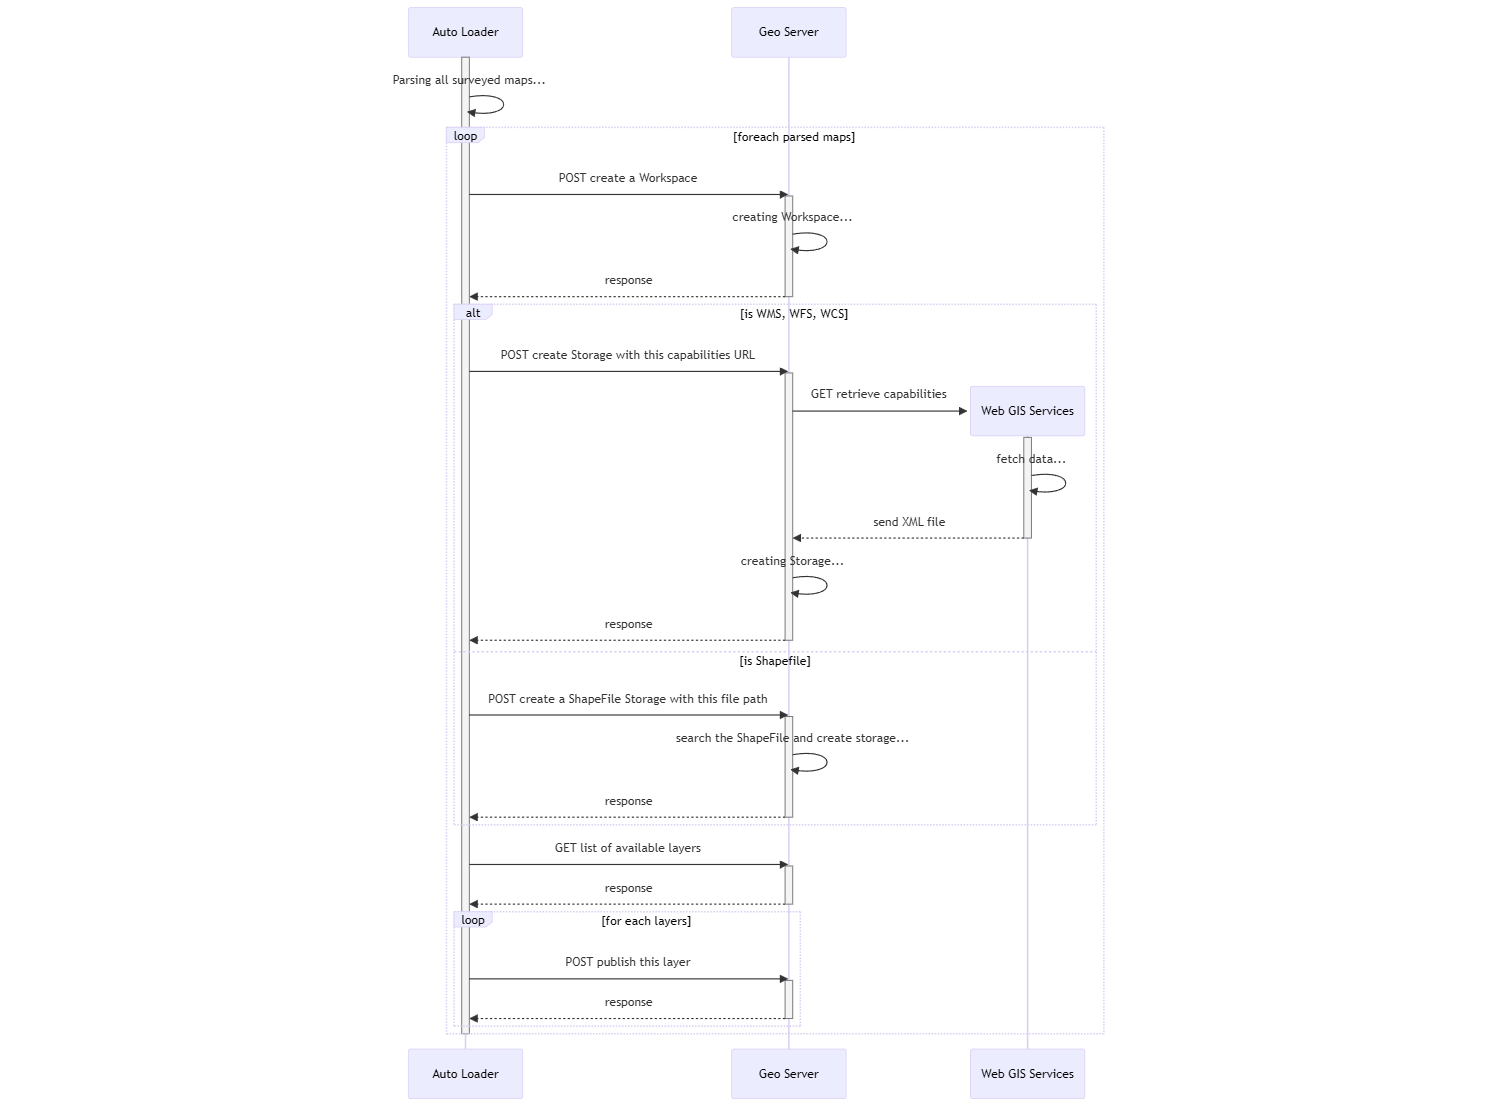
\includegraphics[width=2\textwidth]{Tesi/images/Capitolo6/BmsAutoloaderDiagramFix.png}}%      
      \caption{Ciclo di esecuzione del programma AutoLoader}
      \label{fig:BMSAutoloaderDiagram}      
\end{figure}

\chapter{Integrazione fra Back-end e Front-end}
\label{cap:chapter7}

\section{Programma MapEnumerator}

Sebbene tutte le mappe fossero state caricate all'interno di GeoSever, mediante l'utilizzo del programma AutoLoader, non esisteva alcun meccanismo, fino ad oggi, che informasse il front-end su quali fossero le mappe disponibili e che sistema usare per reperirle. Infatti, il codice esistente realizzato lato front-end prevedeva che si fosse già a conoscenza del tipo di mappa desiderata, oltre a possedere una struttura in cui veniva specificata esattamente la mappa da reperire, non permettendo così di supportare l'aggiunta di nuove mappe. 
\\In questa ultima fase di sviluppo, quindi, l'obiettivo del tirocinante è stato quello sia di realizzare una figura, lato back-end, che potesse memorizzare e comunicare tutte le mappe consultabili, sia quello di implementare, lato front-end, un codice che potesse leggere il contenuto della lista e poi mostrare le mappe a schermo.
\\~\\
L'idea principale per risolvere questo problema è stata quella di realizzare, lato back-end, un programma in C\# che potesse memorizzare all'interno di un database tutte le mappe. È stato poi creato, utilizzando lo standard REST API, un nuovo endpoint in cui fornire la lista completa in formato JSON. Si è poi fornita la possibilità al client di poter interrogare selettivamente la Rest API, facendo uso dei query params, per ottenere informazioni più specifiche (per esempio, chiedere un numero finito di mappe disponibili, oppure l'elenco di mappe filtrato per un certa caratteristica). 
\\Oltre che a fornire l'elenco dei nomi delle mappe, è stato ritenuto adeguato offrire ulteriori informazioni ad esse relative, come il tipo di proiezione geospaziale o il protocollo da utilizzare, così che la mappa potesse essere mostrata correttamente. Infine, questo meccanismo avrebbe dovuto fornire un elenco di mappe non esclusive a un singolo server, come nel caso di GeoServer, ma anche di ulteriori server esterni, come ad esempio la mappa di default fornita da OpenStreetMap. 
\\Per quanto riguarda il front-end, invece, si è preferito realizzare una nuova pagina, in cui richiedere l'elenco delle mappe in formato JSON e successivamente, sfruttando le informazioni ricevute, renderle utilizzabili all'utente.   

\subsection{Struttura del Database}

Il lavoro è dunque iniziato implementando all'interno del back-end un codice che permettesse di memorizzare in maniera persistente la lista delle mappe. Per fare ciò, sono state utilizzate delle librerie apposite fornite direttamente da .NET, le quali hanno permesso di eseguire operazioni sul database, senza la necessità di dover scrivere manualmente query in linguaggio SQL. Facendo uso della classe \verb|ApplicationContex|, la quale estendeva le funzionalità fornite da \verb|DbContext|, è stato quindi possibile creare in automatico una nuova tabella all'interno del database. Quest'ultima è stata realizzata, seguendo la struttura definita in un'altra classe (nota con il nome di \verb|GeoMap|), nel seguente modo:
\begin{itemize}
    \item \verb|Id|: è stato utilizzato come chiave primaria della tabella e conteneva al suo interno tutti gli ID delle mappe. Questi ultimi erano stati generati come GUID anziché come numeri auto incrementati;
    \item \verb|Name|: conteneva i nomi delle mappe che poi il front-end avrebbe utilizzato all'interno dell'applicazione;
    \item \verb|Format|: questo campo serviva per fornire informazioni sul tipo di protocollo da utilizzare al fine di richiedere la mappa correttamente;
    \item \verb|Tags|: questo campo, definito come un array di stringhe, consentiva di dare delle descrizioni sul tipo di mappa memorizzata. Ciò era essenziale per raggruppare le mappe in diverse categorie (come ad esempio "Rischio Frane", "Rischio Alluvioni", ecc..);
    \item \verb|Data|: siccome le informazioni necessarie al front-end per recuperare le mappe dal server variavano a seconda del protocollo scelto e poiché tali informazioni non erano utili al back-end per eseguire eventuali operazioni, è stato deciso di inserire tutte queste informazioni all'interno di un unico campo. Ad esempio, mentre una mappa poteva avere uno stile SLD applicato, un'altra poteva non averne e di conseguenza, i parametri della richiesta da inviare al server di mappe dovevano essere diversi, in modo da richiedere la mappa con lo stile applicato.
    \\Questo campo è stato definito come un oggetto JSON, differente per ogni mappa, che conteneva al suo interno tutte le informazioni necessarie per il front-end al fine di richiedere correttamente quella mappa. Il campo Data di una mappa in formato WMTS era il seguente:
    \begin{lstlisting}[language=Java]{}
    {
       "capabilitiesUrl":"/example.com/?service=WMTS&request=GetCapabilities",
       "layer":"my_layer_name",
       "matrixSet":"EPSG:4326"
    }
    \end{lstlisting}
    \item \verb|CreatedAt|: utilizzato per tenere traccia della data e dell'ora in cui la mappa era stata inserita nel database;
    \item \verb|UpdatedAt|: veniva utilizzato per tenere traccia dell'ultima modifica effettuata sulla riga del database relativa alla mappa;
\end{itemize}

\subsection{Inserimento delle mappe nel Database}

Per aggiungere le mappe all'interno del database, è stato deciso di creare un nuovo comando all'interno del back-end, anch'esso eseguibile tramite CLI. Questo comando, chiamato \verb|'to-database'|, richiedeva come input per il suo funzionamento un file CSV, in modo analogo al comando realizzato per l'AutoLoader.
Questo comando leggeva, in maniera asincrona, tutte le righe all'interno del file e per ognuna di esse creava una nuova entry all'interno del database. Tuttavia, il file utilizzato dal comando \verb|'to-geoserver'| (per caricare gli elementi all'interno del GeoServer), non coincideva con quello utilizzato dal nuovo comando, in quanto era necessario che questo file avesse una struttura analoga a quella della tabella del database.
\\Per realizzare il comando  \verb|'to-database'|, si è fatto nuovamente uso della libreria CSVHelper, la quale ha permesso di far leggere a tale comando il contenuto del file CSV. Purtroppo, tale libreria non supportava nativamente la deserializzazione e la serializzazione del JSON, non riuscendo quindi a estrapolare il contenuto della colonna Data. Per risolvere questo problema, è stato sufficiente introdurre un nuovo tipo di dato riconosciuto dalla libreria CsvHelper. Il tirocinante ha quindi creato una nuova classe che implementava l'interfaccia  \verb|ITypeConverter|, la quale richiedeva a sua volta l'implementazione di due nuovi metodi, uno utilizzato per la serializzazione e uno per la deserializzazione.
\\Per sincronizzare il contenuto delle mappe sul database con quello di GeoServer, il tirocinante ha infine modificato il comando \verb|'to-geoserver'| di modo che, dopo aver inserito le mappe all'interno di GeoServer, avrebbe poi restituito in standard output un nuovo file CSV compatibile con il comando \verb|'to-database'|. Quindi, era possibile eseguire, in sequenza, il comando \verb|'to-geoserver'|, per caricare delle mappe all'interno di GeoServer, e successivamente eseguire \verb|'to-database'|, così da avere le stesse mappe anche sul database.

\subsection{Creazione del servizio Rest API}

Una volta caricate le mappe all'interno del database, è stato quindi necessario realizzare un meccanismo che consentisse di pubblicarle al front-end. Per fare ciò, si è esteso il codice della Rest API già presente all'interno del progetto, avvalendosi delle stesse librerie (fornite dal framework .NET) da loro utilizzate. Precisamente, è stata realizzata una nuova classe, nota con il nome di GeoMapDto (Data Transfer Object), che veniva utilizzata per esporre la struttura della classe GeoMap al front-end. In questo modo, era quindi possibile fornire al front-end solamente una parte delle proprietà della classe GeoMap, mascherando tutte quelle che risultavano superflue al front-end.
\\Successivamente, è stato poi aggiunto un codice che permettesse di eseguire il mapping tra le due classi, riuscendo quindi a convertire un oggetto della classe GeoMapDto a GeoMap, e viceversa: in questo modo era quindi possibile ricevere i dati dal front-end mediante GeoMapDto, convertirli in un oggetto GeoMap e successivamente effettuare eventuali operazioni sul database; la stessa operazione si poteva svolgere anche nella direzione opposta, in modo tale che il back-end potesse inviare dati al front-end. 
\\Infine è stato aggiunto, all'interno della classe che si occupava di gestire tutti gli endpoint della Rest API, un nuovo endpoint apposito per le mappe. Quest'ultimo permetteva di far eseguire al front-end due tipi di richieste, entrambe in GET: la prima, permetteva di recuperare la lista di tutte le mappe disponibili, restituendo tutte le informazioni presenti nelle entries del database; la seconda, invece, permetteva di ricevere informazioni di una singola mappa, a patto che venisse specificato il suo identificativo (GUID). 
La rest API così realizzata rispettava lo standard di OpenAPI 3 e  forniva la sua documentazione attraverso SwaggerUI.
\medskip
\\Per verificare il funzionamento della Rest API, il tirocinante, facendo uso del framework Vitest, ha infine creato una nuova batteria di test che si sarebbe occupata di analizzare ed eseguire tutte le possibili operazioni che un client avrebbe potuto richiede all'endpoint delle mappe. Questi ultimi venivano eseguiti in sequenza ed includevano dei controlli come la quantità di mappe disponibili, la presenza di mappe con tag specifici, il recupero di un numero specifico di mappe, etc...

\subsection{Integrazione front-end della Rest API}

Terminata la parte di scrittura di codice relativa al back-end, il lavoro è poi proseguito verso l'integrazione nel front-end della Rest API, appena sviluppata. Il tirocinante ha scelto di creare una nuova pagina web all'interno dell'applicazione, anziché modificare la pagina, fino ad ora utilizzata, così da preservare il lavoro precedentemente svolto e avere entrambe le implementazioni funzionanti.
\\Innanzitutto, è stato fatto in modo che il front-end riuscisse a contattare il servizio di Rest API per ottenere la lista di mappe. Piuttosto che scrivere manualmente un codice che si occupasse di inviare richieste HTTP asincrone e che estrapolasse il contenuto delle risposte dal back-end, si è optato per l'utilizzo di una libreria apposita. Questa libreria (OpenAPI Generator), analizzando la specifica OpenAPI fornita dalla REST API stessa, permetteva di generare automaticamente del codice TypeScript per contattare il back-end. Da ciò è stato quindi possibile creare un servizio Angular che, utilizzando il codice auto generato, fornisse una serie di metodi utili sia per ottenere l'elenco di tutte le mappe disponibili, sia per ottenere le informazioni su una singola mappa. Questa implementazione, per rappresentare in memoria gli oggetti della mappa (ottenuti come risposta a eventuali richieste), utilizzava una classe che era identica a quella del GeoMapDto (lato back-end).
\\Il lavoro è poi continuato utilizzando i metodi forniti dal servizio Angular, così da riuscire ad inviare richieste HTTP al back-end. L'immagine \ref{fig:restAPI} mostra il contenuto, in formato JSON, della risposta inviata dal servizio di Rest API per ottenere l'elenco delle mappe. 
\begin{figure}[htbp]
      \centering
      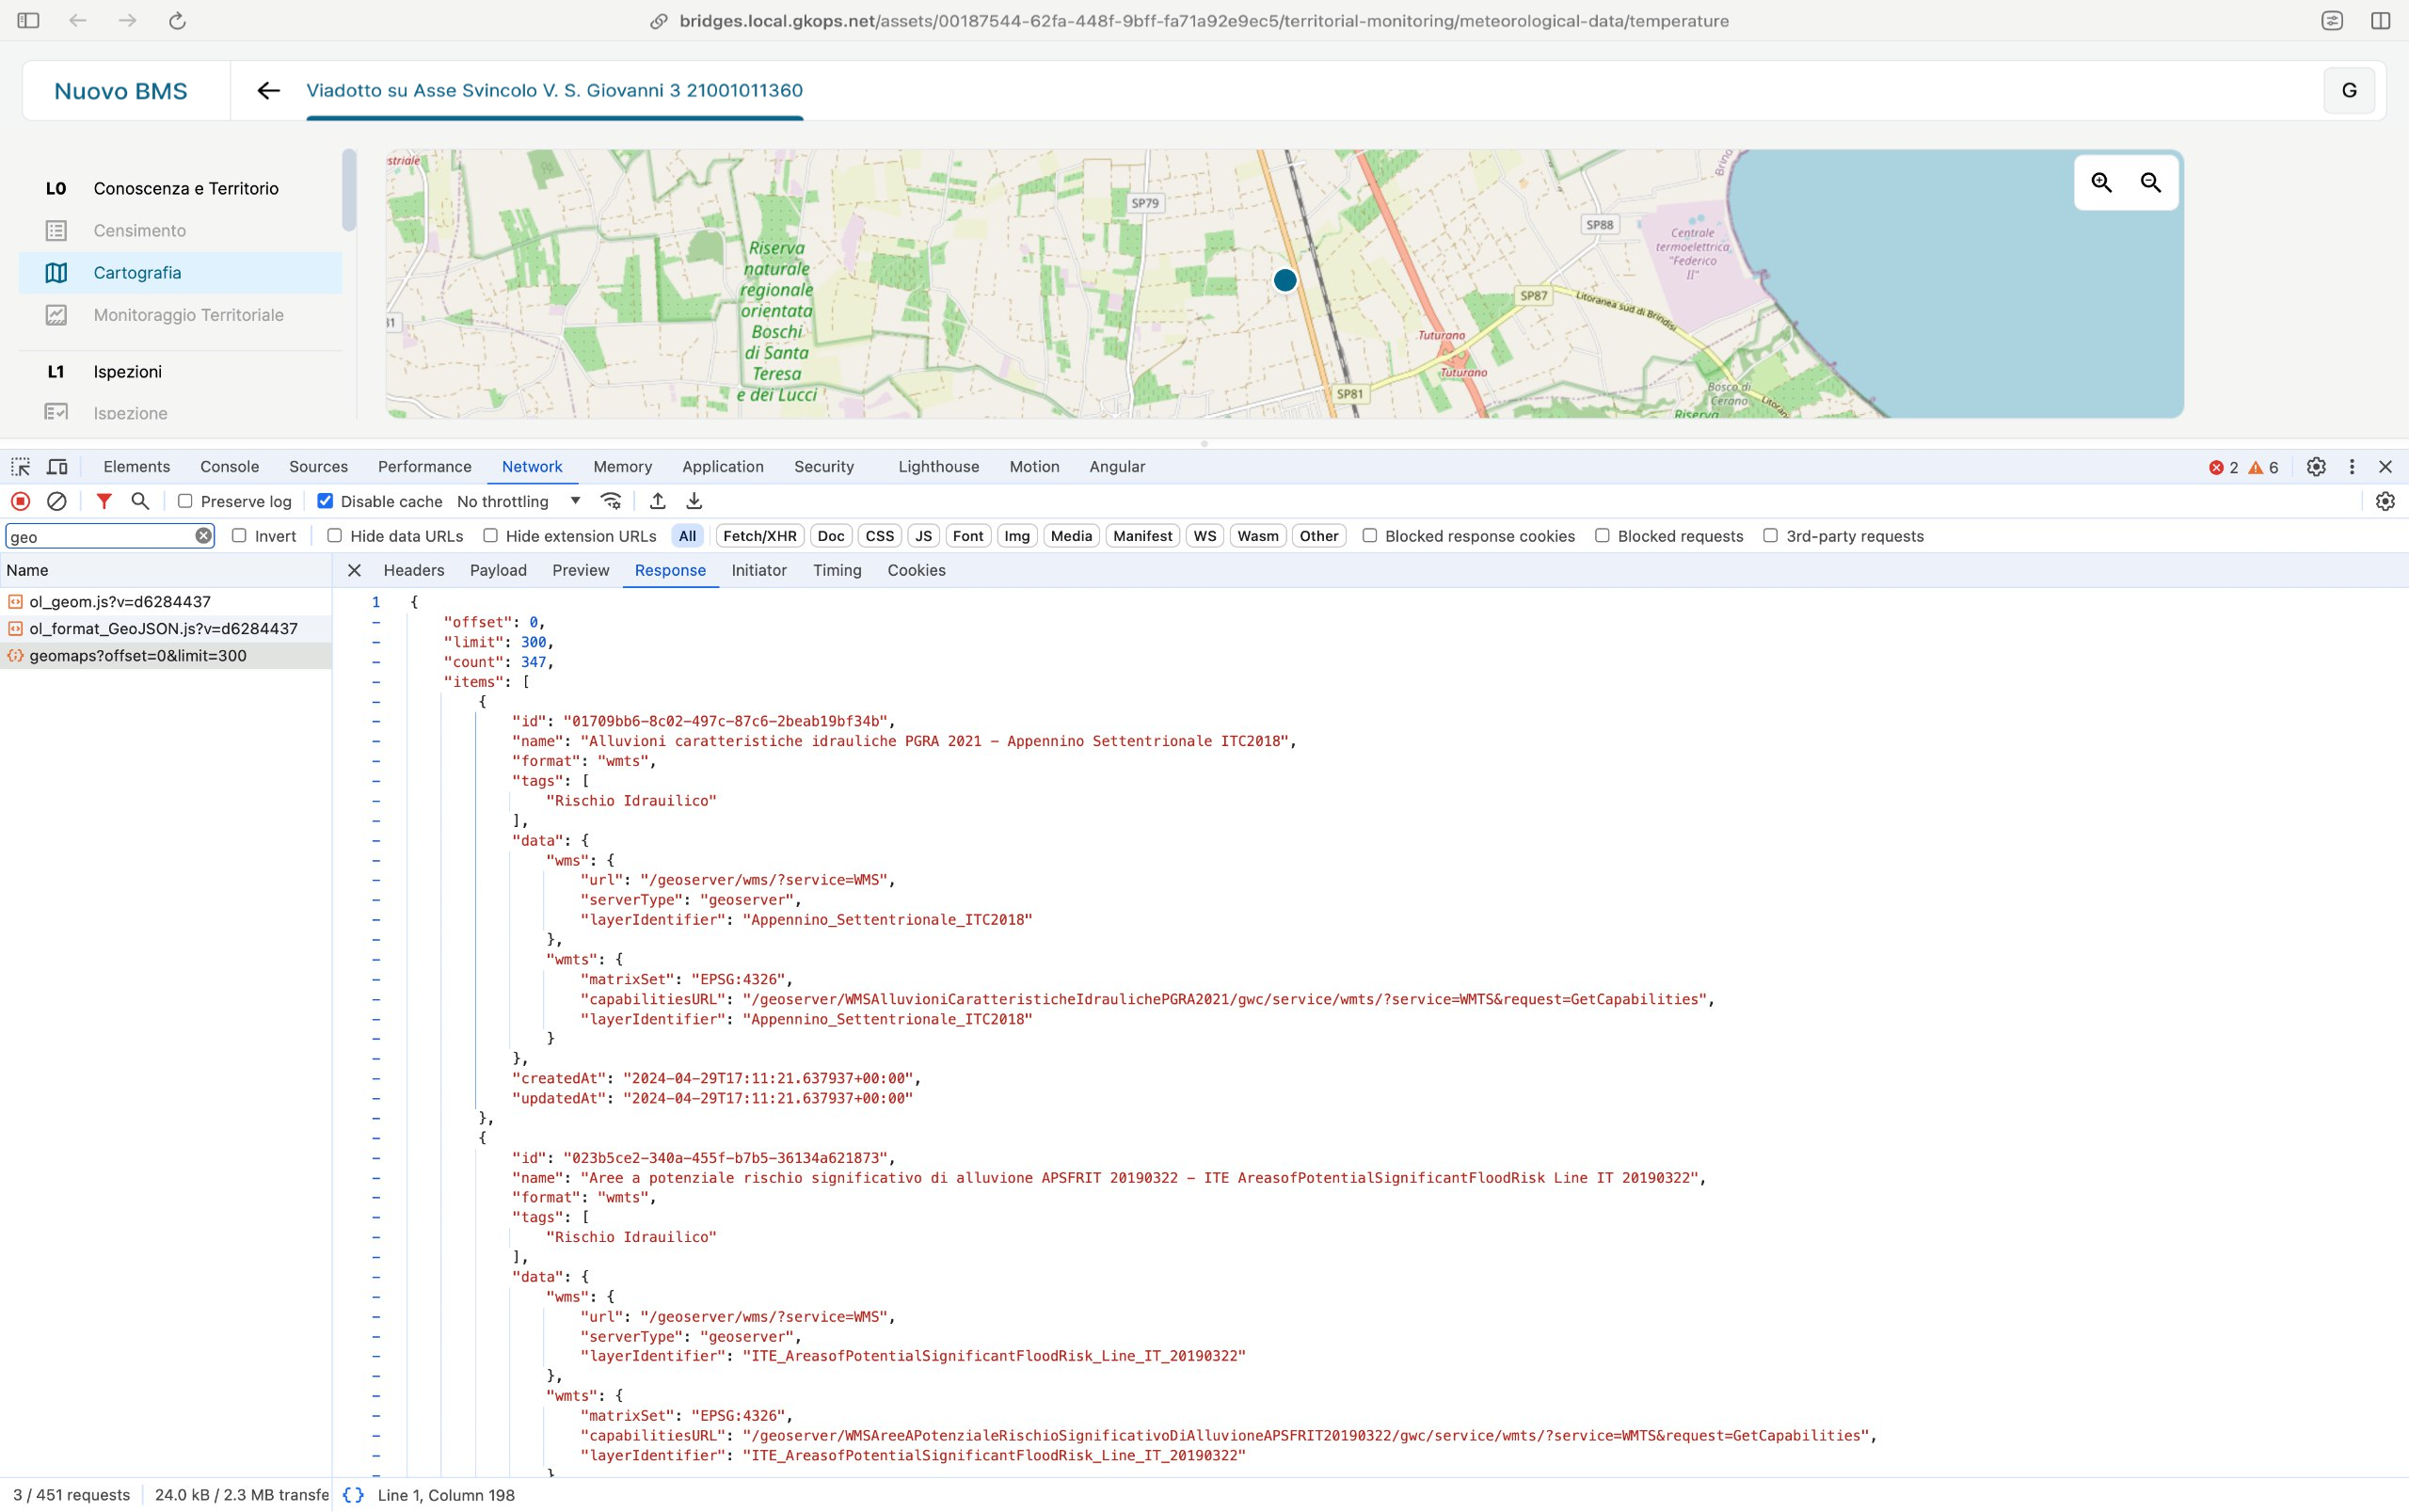
\includegraphics[width=1\textwidth]{Tesi/images/Capitolo7/restAPI.png}
      \caption{Rest API per la lista delle mappe}
      \label{fig:restAPI}
\end{figure}
Come si può osservare nell'immagine, infatti, il campo \verb|Data| varia per ogni mappa e può includere uno o più elementi (come ad esempio \verb|wms| e \verb|wmts|). Ogni elemento contiene a sua volta i parametri necessari per stabilire una corretta comunicazione con il server di mappe, utilizzando gli standard OGC elencati. Il campo \verb|format| specifica il protocollo di preferenza da utilizzare per reperire quella mappa.
\\Inoltre, sono stati resi disponibili dei campi aggiuntivi che permettevano al client di effettuare delle manipolazioni sulla lista delle mappe. Utilizzando il campo "offset", infatti, era possibile specificare il numero di mappe da saltare all'interno dell'elenco prima di ottenere la lista. Con il campo "limit", invece, era possibile specificare il numero massimo di mappe da ottenere dall'API in una singola richiesta. Infine, con il campo "count", il client poteva ottenere informazioni sul numero totale di mappe, senza necessariamente dover leggere il contenuto di ciascuna.
\\~\\
Una volta ottenuta la risposta, è stato quindi necessario realizzare un sistema che permette di leggere il contenuto restituito dal server e successivamente mostrare, nell'interfaccia grafica, l'elenco di mappe con cui l'utente poteva interagire. Per fare ciò, è stato sufficiente manipolare i dati di tipo GeoMapDto, i quali venivano restituiti dai metodi precedentemente utilizzati. Questi dati, lato front-end, sono stati nuovamente inseriti all'interno di una nuova struttura dati, anch'essa di tipo lista. Quest'ultima è stata infine utilizzata per iterare tutte le mappe al suo interno e per ognuna di esse, invocare il metodo buildLayer (della classe buildLayer), passandogli come argomento il riferimento alla mappa iterata. Tuttavia, il metodo buildLayer non richiedeva come argomento una mappa di tipo GeoMapDto, ma, come visto nelle precedenti implementazioni, ne richiedeva una di tipo MapLayer. Quindi, in maniera analoga al back-end, è stato necessario realizzare un "mapper" che si occupasse di convertire il tipo di mappa in GeoMapDto a MapLayer, e viceversa.
Infine, è stata realizzata una sezione apposita che riuscisse a contenere l'elenco di tutte le mappe generate, così da permettere all'utente di poterle selezionare, anche in maniera multipla, attraverso l'uso delle checkbox. In questo modo era possibile far visualizzare più layer contemporaneamente e eventualmente, anche sovrapposti. Nell'immagine \ref{fig:listaMappe} è mostrata l'ultima implementazione dell'interfaccia grafica realizzata dal candidato, contenente la selezione di mappe appena descritta.
\begin{figure}[htbp]
      \centering
      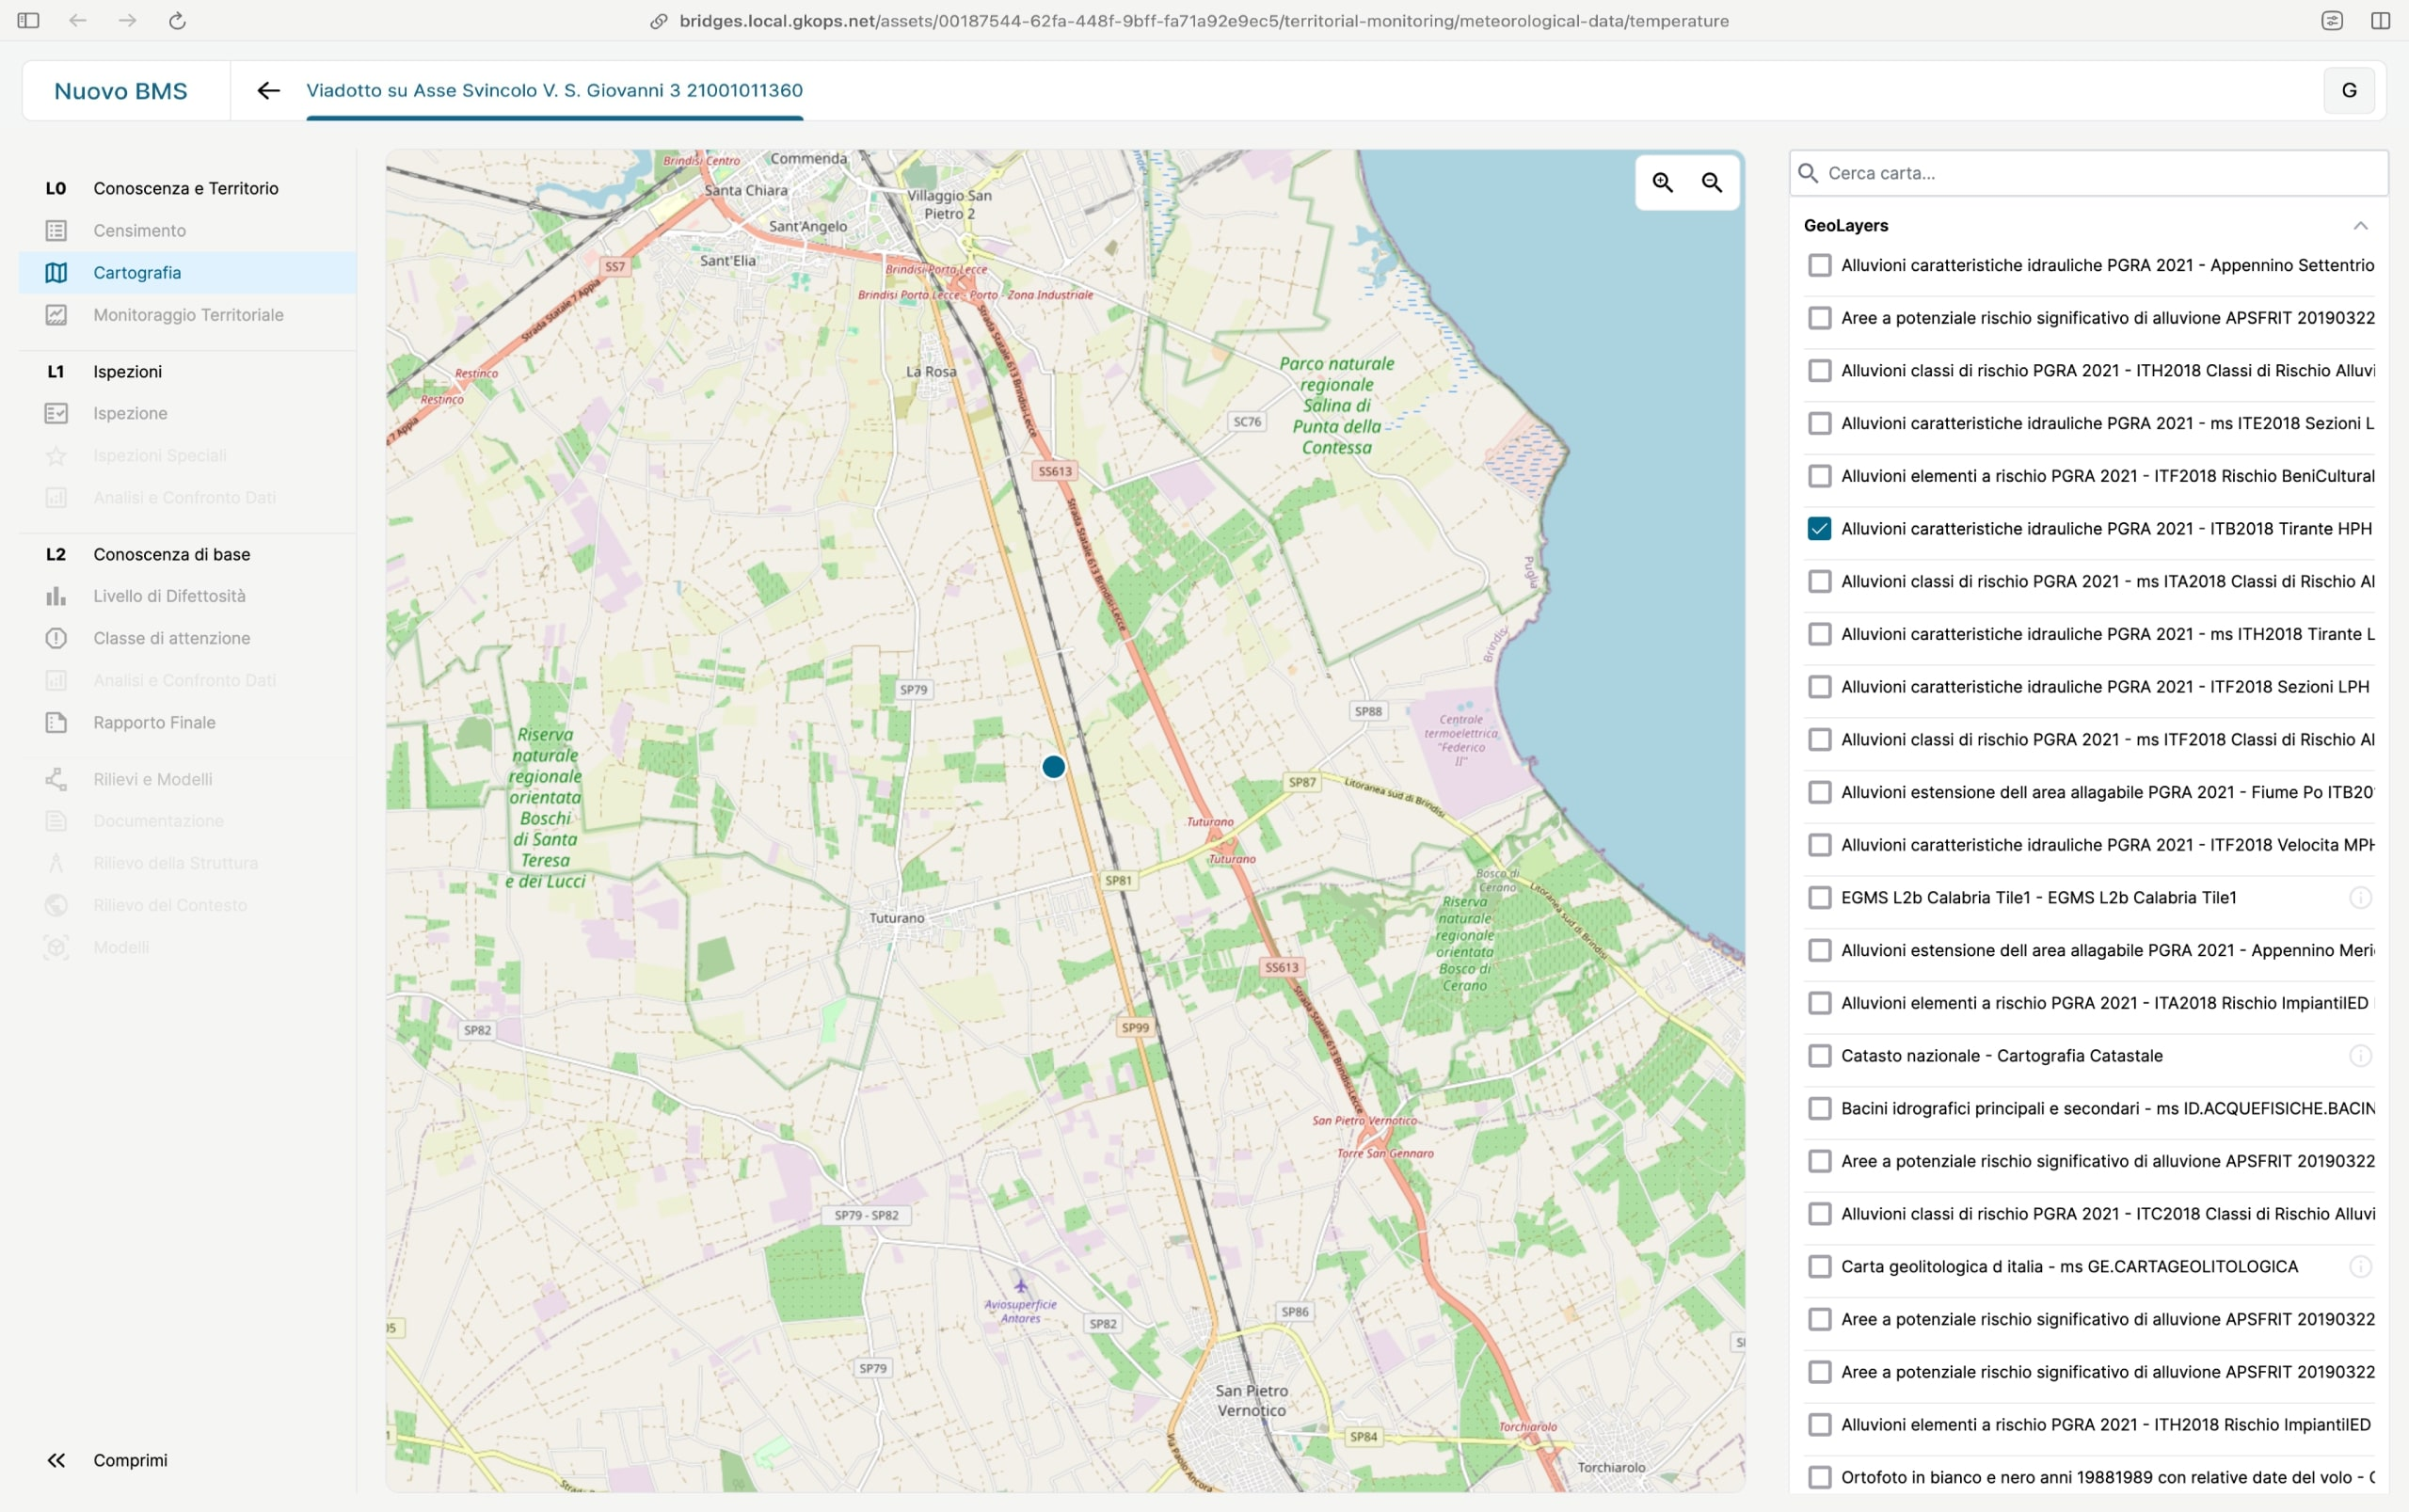
\includegraphics[width=1\textwidth]{Tesi/images/Capitolo7/listaMappe.jpg}
      \caption{Interfaccia grafica per mostrare la lista delle mappe}
      \label{fig:listaMappe}
\end{figure}
\\In conclusione, per spiegare meglio il ciclo di vita effettuato dal front-end e dal back-end, viene mostrato qui sotto l'elenco delle operazioni, eseguite in successione, al fine di ottenere il sistema funzionante:
\begin{enumerate}
    \item back-end: viene eseguito il comando \verb|to-geoserver| per caricare le mappe all'interno del server di mappe.
    \item back-end: viene eseguito il comando \verb|to-database| per inserire  le mappe all'interno del database.
    \item front-end: viene eseguita una richiesta HTTP in GET all'endpoint delle mappe, al fine di ottenere la lista.
    \item back-end: viene eseguita una query verso il database per ottenere la lista delle mappe disponibili.
    \item back-end: la Rest API risponde al client con la lista delle mappe, in formato JSON.
    \item front-end: il client legge il contenuto della lista e mostra graficamente l'elenco.
    \item front-end: quando viene selezionata una mappa, il client contatta il server di mappe per ottenerne i dati.
\end{enumerate}

\chapter{Conclusioni}
\label{cap:chapter8}

\section{Obiettivi raggiunti}

A conclusione del tirocinio, il candidato è riuscito a raggiungere gli obiettivi preposti, sviluppando così un sistema che fosse in grado di fornire e far visualizzare le mappe richieste.
\\Il tirocinante ha infatti iniziato estendendo con successo il componente Angular delle mappe (lato front-end), integrando al suo interno tutti i protocolli OGC richiesti per la trasmissione dei dati geospaziali e ha realizzato una parte all'interno dell'applicazione web che permettesse di testare il funzionamento di tali protocolli, riuscendo a far visualizzare con successo diverse mappe (almeno una per ogni protocollo) e a rappresentarle correttamente nelle loro rispettive proiezioni.
\\Successivamente, ha introdotto nell'applicazione un software con lo scopo di fungere da server di mappe, chiamato GeoServer, il quale è stato utilizzato per la gestione e la distribuzione di questi dati. Nello specifico, ciò ha permesso di memorizzare sia i file locali in formato Shapefile (con i rispettivi file di stile in formato SLD), sia di effettuare proxying dei server OGC esterni, riuscendo anche a fornirli mediante protocollo WMTS, sebbene questi ultimi non lo supportassero. In aggiunta, dopo aver abilitato i suoi meccanismi di cache interna e grazie ai meccanismi di caching configurati nel WebServer (in quanto Reverse Proxy), è stato così possibile risolvere i problemi di rate-limiting e di lentezza riscontrati durante il proxying ai server esterni. 
\\Inoltre, il candidato si è proposto di sviluppare un nuovo programma, noto con il nome di AutoLoader, il quale ha permesso di caricare in automatico tutte le mappe all'interno di GeoServer. Ciò è stato ritenuto necessario dal tirocinante poiché tale procedura risultava molto laboriosa e complessa da effettuare manualmente, sopratutto considerato l'elevato numero di mappe da dover inserire. Per fare ciò, si è fatto uso delle API fornite da GeoServer stesso, le quali, sfortunatamente, non erano state aggiornate dagli sviluppatori con l'evoluzione del software. Il candidato ha quindi dovuto testare manualmente, per ogni richiesta HTTP necessaria, il suo vero funzionamento, così da poter modificare il modo in cui il programma AutoLoader inviava e riceveva le richieste da GeoServer.
\\Infine, è stato poi realizzato un ulteriore programma, lato back-end, il quale ha memorizzato all'interno di un database l'elenco di tutte le mappe disponibili, specificando per ognuna di esse: il nome della mappa, la categoria (rischio frane, alluvioni, etc...) e il modo in cui doveva contattare il server di mappe per reperire il dato, indicandone anche il protocollo OGC da utilizzare. Tutto ciò è stato infine reso disponibile attraverso una Rest API, così da poter esporre tutte queste informazioni al di fuori del back-end. 
\\Successivamente, il candidato ha realizzato un'altra pagina web in grado di contattare il servizio di Rest API, così da richiedere l'elenco di mappe disponibili e, ha reso questa lista visualizzabile all'utente, in modo che potesse selezionare le mappe ed interagire con le stesse.
\medskip
\\Nell'immagine \ref{fig:BMSArchitectureSequenceDiagram} è presente un diagramma di sequenza che espone il funzionamento di tutta l'architettura implementata durante l'intero percorso di tirocinio: essa mostra i passaggi che vengono eseguiti quando un utente accede all'applicazione per richiedere l'elenco di mappe.
\begin{figure}[htbp]
      \centering
      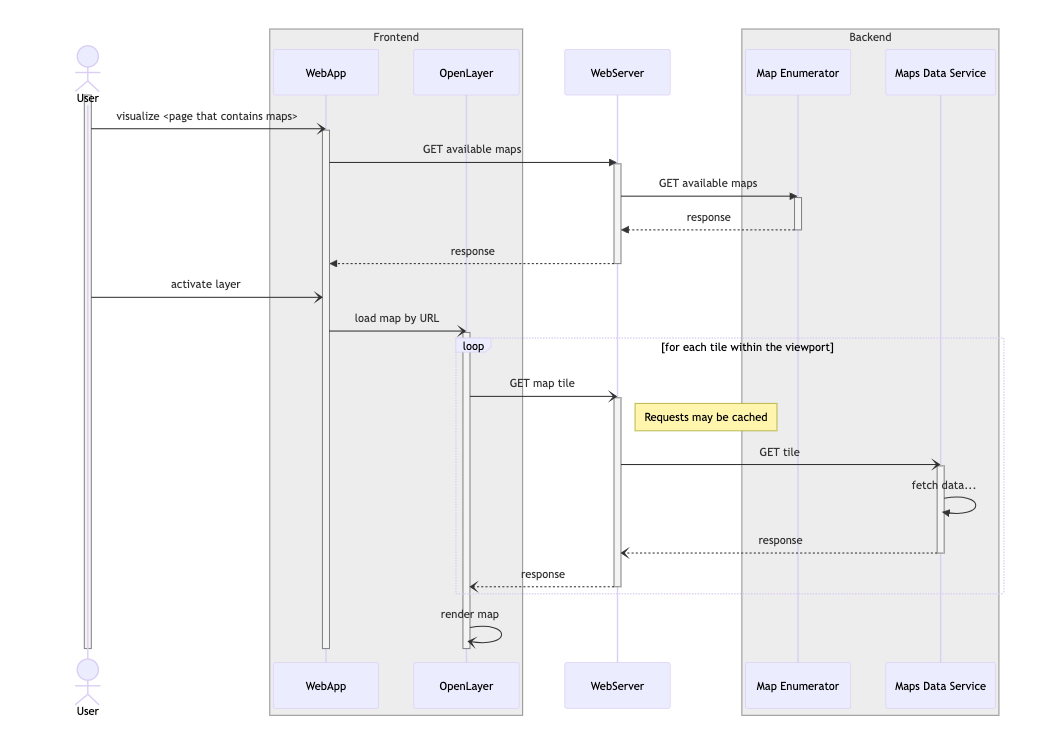
\includegraphics[width=1\textwidth]{Tesi/images/Capitolo8/BMSArchitectureSequenceDiagram.jpg}
      \caption{Diagramma di sequenza che illustra l'architettura realizzata}
      \label{fig:BMSArchitectureSequenceDiagram}
\end{figure}
\\Il client inizia la sua esecuzione inviando una richiesta HTTP al WebServer per ottenere l'elenco completo delle mappe disponibili. Il WebServer, in quanto Reverse Proxy, agisce come intermediario ed inoltra tale richiesta al servizio di Rest API. Una volta ottenuta la risposta, il WebServer la trasmette al client. A questo punto l'interfaccia web dell'applicazione è in grado di visualizzare la lista delle mappe disponibili.
\\Successivamente, una volta che l'utente ha selezionato una mappa specifica, il client, avendo già accesso a tutte le informazioni necessarie, invia una o più richieste HTTP al WebServer, le quali sono formulate in base al tipo di protocollo OGC scelto (per semplificare il diagramma di sequenza, viene mostrato solamente il protocollo WMTS).
Il WebServer, a sua volta, inoltra tali richieste al server di mappe per ottenere i dati richiesti. Dopo aver ottenuto le risposte desiderate, quest'ultimo risponde inviando i dati al WebServer, che a sua volta li trasmette al client. Adesso il client è in grado di visualizzare l'immagine della mappa selezionata. Come viene descritto anche all'interno del diagramma, l'utilizzo del WebServer permette di eseguire caching fra le varie richieste HTTP che vengono inviate.

\section{Riflessioni su sviluppi futuri}

In conclusione, sebbene l'applicazione risulti funzionante, ciò che è stato sviluppato durante il percorso di tirocinio rimane comunque un prototipo. Alla fine del progetto, le mappe non erano ancora state rese disponibili per un ambiente di produzione, in quanto non è ancora stata predisposta una struttura apposita che le possa ospitare. Infatti, le mappe venivano solamente caricate all'interno di un'istanza di GeoServer locale, eccetto durante le presentazioni di alcune demo, in cui veniva utilizzato un server dell'azienda. Inoltre, non era presente alcun meccanismo che permettesse di fornire una mappa proveniente da un server esterno, se quest'ultimo dovesse risultare momentaneamente non disponibile. Durante il periodo di tirocinio, infatti, è accaduto più volte che i servizi esterni andassero in manutenzione o smettessero di funzionare per un lungo periodo di tempo, rendendo così alcune mappe dell'applicazione momentaneamente inutilizzabili. 
\\Per risolvere questo problema, si potrebbe realizzare un meccanismo simile a quello proposto dal candidato precedentemente, sfruttando anche in questo caso le funzionalità offerte da GeoServer. Infatti, oltre ad effettuare proxying dei server esterni, si potrebbe configurare questo software affinché funzioni come mirror, ovvero scarichi localmente tutti i dati ricevuti, così da poter evitare di contattare dei servizi esterni all'azienda. Chiaramente questo meccanismo necessiterebbe di una struttura apposita che sia in grado di ospitare una grande mole di dati, in quanto, come già spiegato precedentemente, il peso dei dati geospaziali può risultare molto elevato.  Un'altra funzionalità che si potrebbe integrare è il supporto al protocollo TMS, il quale, come già ampiamente illustrato all'interno della relazione, potrebbe offrire in alcuni casi delle prestazioni migliori rispetto agli altri protocolli utilizzati; oltre che a offrire una struttura di archiviazione delle tiles, ottimale per l'uso dei servizi Amazon storage S3 e CDN CloudFront. Si potrebbe quindi utilizzare un sistema di servizi Cloud (come AWS) che permetta di supportare tale infrastruttura, archiviando direttamente al loro interno le immagini delle tiles, rappresentanti le mappe. Ciò comporterebbe un aumento delle prestazioni, in modo che il client richieda tramite protocollo TMS (dove possibile) le immagini a tiles, contattando direttamente questi servizi, i quali possono essere scalati in caso di necessità. In aggiunta, poiché l'intera applicazione è stata realizzata utilizzando container Docker, si potrebbe, ove necessario, scalare le loro istanze sia verticalmente, aumentando la potenza di calcolo del singolo servizio, che orizzontalmente, aumentando il numero di istanze contemporanee del servizio stesso. Ciò permetterebbe, ad esempio, di poter aumentare il numero di servizi in parallelo di GeoServer, riuscendo, in caso di necessità, ad ottenere una trasmissione più efficiente dei dati geospaziali mediante i protocolli così implementati.

\chapter*{Ringraziamenti}

Vorrei dedicare questo spazio a esprimere la mia profonda gratitudine a tutte le persone che hanno reso possibile il mio percorso di tirocinio e mi hanno permesso di redigere questa relazione.
\\Innanzitutto, desidero ringraziare il mio tutor aziendale, Andrea Canciani, per la sua guida esperta, la sua instancabile dedizione all'insegnamento e le preziose lezioni che mi ha trasmesso durante questo periodo, nonostante le sue numerose responsabilità. Senza il suo supporto, non avrei potuto acquisire le competenze e le conoscenze necessarie per affrontare le sfide incontrate durante questo percorso di tirocinio.
\\Desidero inoltre ringraziare Alessio Conte, il mio tutor accademico, per il suo sostegno e la sua disponibilità nel guidarmi attraverso le fasi di stesura della relazione.
\\Un ringraziamento va anche a tutti i colleghi dell'azienda, che mi hanno accolto calorosamente e hanno creato un ambiente di lavoro stimolante e collaborativo.
\\Un ringraziamento speciale va al mio insegnante preferito, Vincenzo Gervasi, il quale non solo mi ha concesso l'opportunità di svolgere questo tirocinio, ma è stato un costante punto di riferimento, offrendomi il suo supporto incondizionato, la sua guida preziosa e la sua infinita pazienza. Oltre ad essere un mentore eccezionale ha sempre trovato il tempo di darmi consigli preziosi e di sostenermi in ogni situazione.
\smallskip
\\Desidero esprimere un immenso ringraziamento a Pippo, che considero come un fratello, e che è la persona con cui ho avuto la fortuna di condividere tutti i momenti più importanti della mia vita. In tutti questi anni non mi ha mai lasciato indietro, ha sopportato tutte le mie lamentele (ma sopratutto, non mi ha ancora chiesto i soldi della scommessa persa!), mi ha aiutato in ogni esame di matematica e ha avuto la pazienza di spiegarmi fino all'esasperazione tutto ciò che non capivo. Senza di lui, probabilmente non sarei arrivato dove sono adesso e non potrò mai ringraziarlo abbastanza per questo.
\\E ovviamente un ringraziamento va anche ad Alessio, al contempo sia il miglior compagno di avventure nello spazio, sia la persona migliore con cui potevo legare all'università. Non riuscirò mai a dimenticare tutte le ore passate insieme a studiare, ai consigli ricevuti per la stesura della relazione, alle lezioni private di Elementi di Calcolabilità e Complessità, ma sopratutto alla cronaca in diretta sull'esame di ECC per ricevere il 19 più bello della mia vita! 
\\Un ringraziamento va a Pask e Giova, i miei più cari amici (ormai palesemente adottati) con cui ho condiviso passioni e interessi  sin dai tempi di Warhammer 40k.
\\Voglio ringraziare inoltre Emax e Gianlo, con i quali ho condiviso fin dai primi momenti la passione per l'informatica.
\\Ringrazio ovviamente Matte, Piersa, Buoni, Ricca, Gianluca, Lorenzo, Edoardo, Corti, Marra, Tani, Lea e tutti gli altri miei amici (siete troppi, non posso mettere tutti i nomi perché sicuramente mi scorderei qualcuno) che mi sono comunque rimasti vicini nonostante scomparissi per lunghi periodi a causa degli impegni universitari.
\\Un altro ringraziamento va anche ai miei compagni di superiori nonché colleghi universitari Jacopo, Gine e Nicco, con cui abbiamo condiviso i primi anni di università (ma soprattutto tanta crema al pistacchio!).
\smallskip
\\Come posso non ringraziare Monica che, nonostante tutti i miei difetti, continua a starmi affianco ogni giorno. Grazie per il tuo amore, il tuo sostegno, per avermi aiutato tutto questo tempo, per aver trascorso intere giornate a vedermi scrivere la relazione solo per poter passare del tempo insieme, ma soprattutto per la tua infinita pazienza (anche se molte volte non è colpa mia eh, sei tu che fai schifo a lol e mi uccidi nei videogiochi!). 
\\Concludo con l'ultimo ringraziamento che va a tutta la mia famiglia, nello specifico ai miei super genitori e a mia sorella un po' antipatica, i quali ormai hanno palesemente dimostrato di essere arrivati all'esasperazione e non credo mi avrebbero sopportato ancora per molto se non mi fossi laureato. Grazie per avermi sempre sostenuto, anche quando ero un po' insopportabile.
\begin{flushright}
Samuele Calugi
\end{flushright}
\thispagestyle{empty}

%\appendix

%\include{chapters/AppendiceA}

\bibliographystyle{plain}
\bibliography{chapters/Bibliografia.bib}

\end{document}
% -----------------------------------------------------------------
